\documentclass{article}
\usepackage{isabelle,isabellesym}
\renewcommand{\ttdefault}{cmtt}
\usepackage{csquotes}
\usepackage{enumitem}

\newlist{inlinelist}{enumerate*}{1}
\setlist*[inlinelist,1]{%
  label=(\roman*),
}
\usepackage{hyperref}
\usepackage[numbers]{natbib}
\usepackage{amsmath}
%\usepackage{amsthm}
\usepackage{amsfonts}
\usepackage{amssymb}
%\usepackage{bbm}  % Para el \bb{1}
%\usepackage[numbers]{natbib}
\usepackage{enumitem}
\usepackage{babel}
%\usepackage{babelbib}
\usepackage{multidef}
\usepackage{verbatim}
\usepackage{stmaryrd} %% para \llbracket
%%
%% \usepackage[bottom=2cm, top=2cm, left=2cm, right=2cm]{geometry}
%% \usepackage{titling}
%% \setlength{\droptitle}{-10ex} 
%%
\renewcommand{\o}{\vee}
\renewcommand{\O}{\bigvee}
\newcommand{\y}{\wedge}
\newcommand{\Y}{\bigwedge}
\newcommand{\limp}{\rightarrow}
\newcommand{\lsii}{\leftrightarrow}
%%

\DeclareMathOperator{\cf}{cf}
\DeclareMathOperator{\dom}{dom}
\DeclareMathOperator{\im}{img}
\DeclareMathOperator{\Fn}{Fn}
\DeclareMathOperator{\rk}{rk}
\DeclareMathOperator{\mos}{mos}
\DeclareMathOperator{\trcl}{trcl}
\DeclareMathOperator*{\diag}{\bigtriangleup}
\DeclareMathOperator{\Con}{Con}
\DeclareMathOperator{\Club}{Club}


\newcommand{\modelo}[1]{\mathbf{#1}}
\newcommand{\axiomas}[1]{\mathit{#1}}
\newcommand{\clase}[1]{\mathsf{#1}}
\newcommand{\poset}[1]{\mathbb{#1}}
\newcommand{\operador}[1]{\mathbf{#1}}

%% \newcommand{\Lim}{\clase{Lim}}
%% \newcommand{\Reg}{\clase{Reg}}
%% \newcommand{\Card}{\clase{Card}}
%% \newcommand{\On}{\clase{On}}
%% \newcommand{\WF}{\clase{WF}}
%% \newcommand{\HF}{\clase{HF}}
%% \newcommand{\HC}{\clase{HC}}
%%
%% El siguiente comando reemplaza todos los anteriores:
%%
\multidef{\clase{#1}}{Card,HC,HF,Lim,On->Ord,Reg,WF,Ord}
\newcommand{\ON}{\On}

%% En lugar de usar todo el paquete bbm:
\DeclareMathAlphabet{\mathbbm}{U}{bbm}{m}{n} 
\newcommand{\1}{\mathbbm{1}}

%%
%% \newcommand{\calD}{\mathcal{D}}
%% \newcommand{\calS}{\mathcal{S}}
%% \newcommand{\calU}{\mathcal{U}}
%% \newcommand{\calB}{\mathcal{B}}
%% \newcommand{\calL}{\mathcal{L}}
%% \newcommand{\calF}{\mathcal{F}}
%% \newcommand{\calT}{\mathcal{T}}
%% \newcommand{\calW}{\mathcal{W}}
%% \newcommand{\calA}{\mathcal{A}}
%%
%% El siguiente comando reemplaza todos los anteriores:
%%
\multidef[prefix=cal]{\mathcal{#1}}{A-Z}
%%
%% \newcommand{\A}{\modelo{A}}
%% \newcommand{\BB}{\modelo{B}}
%% \newcommand{\ZZ}{\modelo{Z}}
%% \newcommand{\PP}{\modelo{P}}
%% \newcommand{\QQ}{\modelo{Q}}
%% \newcommand{\RR}{\modelo{R}}
%%
%% El siguiente comando reemplaza todos los anteriores:
%%
\multidef{\modelo{#1}}{A,BB->B,CC->C,NN->N,PP->P,QQ->Q,RR->R,ZZ->Z}

\multidef[prefix=p]{\mathbb{#1}}{A-Z}
%% \newcommand{\B}{\modelo{B}}
%% \newcommand{\C}{\modelo{C}}
%% \newcommand{\F}{\modelo{F}}
%% \newcommand{\D}{\modelo{D}}

\newcommand{\Th}{\mb{Th}}
\newcommand{\Mod}{\mb{Mod}}

\newcommand{\Se}{\operador{S^\prec}}
\newcommand{\Pu}{\operador{P_u}}
\renewcommand{\Pr}{\operador{P_R}}
\renewcommand{\H}{\operador{H}}
\renewcommand{\S}{\operador{S}}
\newcommand{\I}{\operador{I}}
\newcommand{\E}{\operador{E}}

\newcommand{\se}{\preccurlyeq}
\newcommand{\ee}{\succ}
\newcommand{\id}{\approx}
\newcommand{\subm}{\subseteq}
\newcommand{\ext}{\supseteq}
\newcommand{\iso}{\cong}
%%
\renewcommand{\emptyset}{\varnothing}
\newcommand{\rel}{\mathcal{R}}
\newcommand{\Pow}{\mathop{\mathcal{P}}}
\renewcommand{\P}{\Pow}
\newcommand{\BP}{\mathrm{BP}}
\newcommand{\func}{\rightarrow}
\newcommand{\ord}{\mathrm{Ord}}
\newcommand{\R}{\mathbb{R}}
\newcommand{\N}{\mathbb{N}}
\newcommand{\Z}{\mathbb{Z}}
\renewcommand{\I}{\mathbb{I}}
\newcommand{\Q}{\mathbb{Q}}
\newcommand{\B}{\mathbf{B}}
\newcommand{\<}{\langle}
\renewcommand{\>}{\rangle}
\newcommand{\lb}{\langle}
\newcommand{\rb}{\rangle}
\newcommand{\impl}{\rightarrow}
\newcommand{\ent}{\Rightarrow}
\newcommand{\tne}{\Leftarrow}
\newcommand{\sii}{\Leftrightarrow}
\renewcommand{\phi}{\varphi}
\newcommand{\phis}{{\varphi^*}}
\renewcommand{\th}{\theta}
\newcommand{\Lda}{\Lambda}
\newcommand{\La}{\Lambda}
\newcommand{\lda}{\lambda}
\newcommand{\ka}{\kappa}
\newcommand{\del}{\delta}
\newcommand{\de}{\delta}
\newcommand{\ze}{\zeta}
%\newcommand{\ }{\ }
\newcommand{\la}{\lambda}
\newcommand{\al}{\alpha}
\newcommand{\be}{\beta}
\newcommand{\ga}{\gamma}
\newcommand{\Ga}{\Gamma}
\newcommand{\ep}{\varepsilon}
\newcommand{\De}{\Delta}
\newcommand{\defi}{\mathrel{\mathop:}=}
\newcommand{\forces}{\Vdash}
%\newcommand{\ap}{\mathbin{\wideparen{\ }}}
\newcommand{\Tree}{{\mathrm{Tr}_\N}}
\newcommand{\PTree}{{\mathrm{PTr}_\N}}
\newcommand{\NWO}{\mathit{NWO}}
\newcommand{\Suc}{{\N^{<\N}}}%
\newcommand{\init}{\mathsf{i}}
\newcommand{\ap}{\mathord{^\smallfrown}}
\newcommand{\Cantor}{\mathcal{C}}
%\newcommand{\C}{\Cantor}
\newcommand{\Baire}{\mathcal{N}}
\newcommand{\sig}{\ensuremath{\sigma}}
\newcommand{\fsig}{\ensuremath{F_\sigma}}
\newcommand{\gdel}{\ensuremath{G_\delta}}
\newcommand{\Sig}{\ensuremath{\boldsymbol{\Sigma}}}
\newcommand{\bPi}{\ensuremath{\boldsymbol{\Pi}}}
\newcommand{\Del}{\ensuremath{\boldsymbol\Delta}}
%\renewcommand{\F}{\operador{F}}
\newcommand{\ths}{{\theta^*}}
\newcommand{\om}{\ensuremath{\omega}}
%\renewcommand{\c}{\complement}
\newcommand{\comp}{\mathsf{c}}
\newcommand{\co}[1]{\left(#1\right)^\comp}
\newcommand{\len}[1]{\left|#1\right|}
\DeclareMathOperator{\tlim}{\overline{\mathrm{TLim}}}
\newcommand{\card}[1]{{\left|#1\right|}}
\newcommand{\bigcard}[1]{{\bigl|#1\bigr|}}
%
% Cardinality
%
\newcommand{\lec}{\leqslant_c}
\newcommand{\gec}{\geqslant_c}
\newcommand{\lc}{<_c}
\newcommand{\gc}{>_c}
\newcommand{\eqc}{=_c}
\newcommand{\biy}{\approx}
\newcommand*{\ale}[1]{\aleph_{#1}}
%
\newcommand{\Zerm}{\axiomas{Z}}
\newcommand{\ZC}{\axiomas{ZC}}
\newcommand{\AC}{\axiomas{AC}}
\newcommand{\DC}{\axiomas{DC}}
\newcommand{\MA}{\axiomas{MA}}
\newcommand{\CH}{\axiomas{CH}}
\newcommand{\ZFC}{\axiomas{ZFC}}
\newcommand{\ZF}{\axiomas{ZF}}
\newcommand{\Inf}{\axiomas{Inf}}
%
% Cardinal characteristics
%
\newcommand{\cont}{\mathfrak{c}}
\newcommand{\spl}{\mathfrak{s}}
\newcommand{\bound}{\mathfrak{b}}
\newcommand{\mad}{\mathfrak{a}}
\newcommand{\tower}{\mathfrak{t}}
%
\renewcommand{\hom}[2]{{}^{#1}\hskip-0.116ex{#2}}
\newcommand{\pred}[1][{}]{\mathop{\mathrm{pred}_{#1}}}
%% Postfix operator with supressable space:
%% \newcommand*{\iseg}{\relax\ifnum\lastnodetype>0 \mskip\medmuskip\fi{\downarrow}} %
\newcommand*{\iseg}{{\downarrow}}
\newcommand{\rr}{\mathrel{R}}
\newcommand{\restr}{\upharpoonright}
%\newcommand{\type}{\mathtt{}}
\newcommand{\app}{\mathop{\mathrm{Aprox}}}
\newcommand{\hess}{\triangleleft}
\newcommand{\bx}{\bar{x}}
\newcommand{\by}{\bar{y}}
\newcommand{\bz}{\bar{z}}
\newcommand{\union}{\mathop{\textstyle\bigcup}}
\newcommand{\sm}{\setminus}
\newcommand{\sbq}{\subseteq}
\newcommand{\nsbq}{\subseteq}
\newcommand{\mty}{\emptyset}
\newcommand{\dimg}{\text{\textup{``}}} % direct image
\newcommand{\quine}[1]{\ulcorner{\!#1\!}\urcorner}
%\newcommand{\ntrm}[1]{\textsl{\textbf{#1}}}
\newcommand{\Null}{\calN\!\mathit{ull}}
\DeclareMathOperator{\club}{Club}
\DeclareMathOperator{\otp}{otp}

%%%%%%%%%%%%%%%%%%%%%%%%%
% Variant aleph, beth, etc
% From http://tex.stackexchange.com/q/170476/69595
\makeatletter
\@ifpackageloaded{txfonts}\@tempswafalse\@tempswatrue
\if@tempswa
  \DeclareFontFamily{U}{txsymbols}{}
  \DeclareFontFamily{U}{txAMSb}{}
  \DeclareSymbolFont{txsymbols}{OMS}{txsy}{m}{n}
  \SetSymbolFont{txsymbols}{bold}{OMS}{txsy}{bx}{n}
  \DeclareFontSubstitution{OMS}{txsy}{m}{n}
  \DeclareSymbolFont{txAMSb}{U}{txsyb}{m}{n}
  \SetSymbolFont{txAMSb}{bold}{U}{txsyb}{bx}{n}
  \DeclareFontSubstitution{U}{txsyb}{m}{n}
  \DeclareMathSymbol{\aleph}{\mathord}{txsymbols}{64}
  \DeclareMathSymbol{\beth}{\mathord}{txAMSb}{105}
  \DeclareMathSymbol{\gimel}{\mathord}{txAMSb}{106}
  \DeclareMathSymbol{\daleth}{\mathord}{txAMSb}{107}
\fi
\makeatother

%%%%%%%%%%%%%%%%%%%%%%%%%%%%%%%%%%%%%%%%%%%%%%%%%%%%%%%%%%%%
%%
%% Theorem Environments
%%
%% \newtheorem{theorem}{Theorem}
%% \newtheorem{lemma}[theorem]{Lemma}
%% \newtheorem{prop}[theorem]{Proposition}
%% \newtheorem{corollary}[theorem]{Corollary}
%% \newtheorem{claim}{Claim}
%% \newtheorem*{claim*}{Claim}
%% \theoremstyle{definition}
%% \newtheorem{definition}[theorem]{Definition}
%% \newtheorem{remark}[theorem]{Remark}
%% \newtheorem{example}[theorem]{Example}
%% \theoremstyle{remark}
%% \newtheorem*{remark*}{Remark}
%%
%%%%%%%%%%%%%%%%%%%%%%%%%%%%%%%%%%%%%%%%%%%%%%%%%%%%%%%%%%%%%%%%%%%%%%

%% \newenvironment{inducc}{\begin{list}{}{\itemindent=2.5em \labelwidth=4em}}{\end{list}}
%% \newcommand{\caso}[1]{\item[\fbox{#1}]}
\newenvironment{proofofclaim}{\begin{proof}[Proof of Claim]}{\end{proof}}


%%% Local Variables: 
%%% mode: latex
%%% TeX-master: "first_steps_into_forcing"
%%% End: 

\makeatletter
\def\foottext{\gdef\@thefnmark{}\@footnotetext}
\makeatother
\newcommand{\keywords}[1]{\foottext{\emph{Keywords:} #1}}
\newcommand{\ack}[1]{\par\bigskip \noindent \emph{Acknowledgment:} #1}

\begin{document}
\title{Separation in Generic Extensions for Isabelle}
\author{Emmanuel Gunther
  \and 
  Miguel Pagano
  \and 
  Pedro S\'anchez Terraf}
\maketitle

\begin{abstract}
  We mechanize, in the proof assistant
  Isabelle, a proof of the
  axiom-scheme of Separation in 
  generic extensions of models of set theory  
  by using the fundamental theorems of forcing.
  We also formalize the satisfaction of the axioms of
  Extensionality, Foundation, Union, and Powerset. The axiom of
  Infinity is likewise treated, under additional assumptions on the ground
  model.
  We also  extend Paulson's library on constructibility  with
  renaming of variables for internalized formulas, an improvement on
  definitions by recursion on well-founded  relations and sharpening
  of the hypotheses in his development of relativization and
  absoluteness.
\end{abstract}
\keywords{
Isabelle/ZF, forcing, names, generic extension, constructibility.
}

%%%%%%%%%%%%%%%%%%%%%%%%%%%%%%%%%%%%%%%%%%%%%%%%%%%%%%%%%%%%%%%%%%%%%%%%%%%%%%%%
%%%%%%%%%%%%%%%%%%%%%%%%%%%%%%%%%%%%%%%%%%%%%%%%%%%%%%%%%%%%%%%%%%%%%%          
\section{Introduction}
% no \IEEEPARstart
Zermelo-Fraenkel Set Theory ($\ZF$) has a prominent place among formal
theories; in particular, it provides a foundation for mathematics and
most of the formal toolkit used everyday by the computer scientist has
also Set Theory at its base (cf.~\cite{paulson1995set}). In this time
of mechanization of mathematics~\cite{avigad2018mechanization}, it
seems natural to ask for a mechanization of the most salient results
of Set Theory.

After G\"odel's Incompleteness Theorems, we cannot expect to have a
formal proof of the consistency of Set Theory in $\ZF$. Besides its own
consistency, there are other results which are undecided by $\ZF$: the
undecidability of Continuum Hypothesis leads to the development of
techniques for independence proofs. First G\"odel introduced the
theory of \emph{inner models}, which gives rise to his model $L$ of
the \emph{Axiom of Constructibility} \cite{godel-L} and proved the
relative consistency of the Axiom of Choice and the Generalized
Continuum Hypothesis with $\ZF$. Thirty years later Paul
J. Cohen~\cite{Cohen-CH-PNAS} devised the technique of \emph{forcing},
which is the only known way of \emph{extending} models of $\ZF$; in
particular, it can be used to prove the relative consistency of the
negation of the Continuum Hypothesis. 

In this work we address a substantial part of formalizing the proof
that given a model $M$ of $\ZF$, any \emph{generic extension} $M[G]$
given by forcing also satisfies $\ZF$. As remarked by
\citet[][p.250]{kunen2011set} \enquote{[...] in verifying that $M[G]$
  is a model for set theory, the hardest axiom to verify is
  Comprehension.}  The most important achievement of this paper is the
mechanization in Isabelle a considerable part of this result; en route
to this, we also formalized the satisfaction by $M[G]$ of
Extensionality, Foundation, Union, and Infinity.

Our development benefited from the remarkable work done by Lawrence
Paulson \cite{paulson_2003} on the formalization of G\"odel's
constructible universe in the proof assistant \emph{Isabelle}. The
ultimate goal of our project is the formalization of forcing to
complete the mechanization of the independence of the Continuum
Hypothesis. We think that this project constitutes an interesting case
which stresses how feasible is to formally implement mathematics that
involve several levels of reasoning.

The \emph{Formal Abstract} project~\cite{hales-fabstracts} proposes
that the mechanization of mathematics can advance by formalizing some
main result under the explicit assumption of the material
(definitions, propositions, lemmas) on which it is based. In line with
this advice, we profited that the proof that those axioms hold in
generic extension is independent of the \emph{proofs} of the
``fundamental'' theorems of forcing. Let us remark that the definition
of the forces relation is, by itself, quite demanding; the
formalization of it and of the fundamental theorems of forcing roughly
comprises little less than a half of our full project.

It might be a little surprising the lack of formalizations of forcing
and generic extensions. As far as we know, the development of
\citet{JFR6232} in homotopy type theory for constructing generic
extensions in a sheaf-theoretic setting is the unique mechanization of
forcing. This contrast with the fruitful use of forcing techniques to
extend the Curry-Howard isomorphism to classical axioms
\cite{Miquel:2011:FPT:2058525.2059614,lmcs:1070}. Moreover, the
combination of forcing with intuitionistic type theory
\cite{coquand2010note} gives rise both to positive results (an
algorithm to obtain witnesses of the continuity of definable
functionals \cite{coquand2012computational}) and also negative
(the independence of Markov's principle \cite{lmcs:3859}).

% moreover forcing translations \cite{jaber:hal-01319066}.

\fbox{Parece mucho comienzo sólo para introducir a Kunen}
\fbox{¿lo puedo achurar un poco?}

In a gross simplification, there are two aspects to a formalization
project like this one: thematic and programmatic. The first concerns
the handling of all the theoretical concepts and results in the
subject, while the second involves the practical issues of the
implementation and design. In the case of forcing, the main intricacy
lies in the first aspect. In this sense, following a sensible
presentation of the material is key.  The authoritative reference 
on the subject during the last 30 years has been Kunen's classical
\cite{kunen1980}. In our
formalizaton we have followed a recent rewrite \cite{kunen2011set}
of that  textbook, which presents the material in the same sharp 
style but offering a lot of details. In some sense this project
wouldn't exist without this book. As alternative, introductory
resources, the  interested reader can check
\cite{chow-beginner-forcing}; also, the book \cite{weaver2014forcing}
contains a thorough treament minimizing the technicalities.

We briefly describe the contents of each
section. Section~\ref{sec:isabelle} contains the bare minimun
requirements to understand the (meta)logics used in Isabelle. Next, an
overview of the model theory of set theory is presented in
Section~\ref{sec:axioms-models-set-theory}. There is an ``internal''
representation of first-order formulas as sets, implemented by
Paulson; Section~\ref{sec:renaming} discusses syntactical
transformations of the former, mainly permutation of variables. 
In Section~\ref{sec:generic-extensions} the generic extensions are
succintly reviewed and how the treatment of well founded recursion in
Isabelle was enhanced. We take care of the ``easy axioms'' in
Section~\ref{sec:easy-axioms}; these are the ones that
do not depend on the forcing theorems. We describe the latter in
Section~\ref{sec:forcing}. We adapted the  work by Paulson to our
needs, and this is described in
Section~\ref{sec:hack-constructible}. We present the proof
of the Separation Axiom Scheme in Section~\ref{sec:proof-separation},
which follows closely its implementation. A plan for future work and
some immediate conclusions are offered in
Section~\ref{sec:conclusions-future-work}.

%%% Local Variables: 
%%% mode: latex
%%% TeX-master: "Separation_In_MG"
%%% ispell-local-dictionary: "american"
%%% End: 


%%
%% macros for Isabelle generated LaTeX output
%%

%%% Simple document preparation (based on theory token language and symbols)

% isabelle environments

\newcommand{\isabellecontext}{UNKNOWN}
\newcommand{\setisabellecontext}[1]{\def\isabellecontext{#1}}

\newcommand{\isastyle}{\UNDEF}
\newcommand{\isastylett}{\UNDEF}
\newcommand{\isastyleminor}{\UNDEF}
\newcommand{\isastyleminortt}{\UNDEF}
\newcommand{\isastylescript}{\UNDEF}
\newcommand{\isastyletext}{\normalsize\rm}
\newcommand{\isastyletxt}{\rm}
\newcommand{\isastylecmt}{\rm}

\newcommand{\isaspacing}{%
  \sfcode 42 1000 % .
  \sfcode 63 1000 % ?
  \sfcode 33 1000 % !
  \sfcode 58 1000 % :
  \sfcode 59 1000 % ;
  \sfcode 44 1000 % ,
}

%symbol markup -- \emph achieves decent spacing via italic corrections
\newcommand{\isamath}[1]{\emph{$#1$}}
\newcommand{\isatext}[1]{\emph{#1}}
\DeclareRobustCommand{\isascriptstyle}{\def\isamath##1{##1}\def\isatext##1{\mbox{\isaspacing\isastylescript##1}}}
\newcommand{\isactrlsub}[1]{\emph{\isascriptstyle${}\sb{#1}$}}
\newcommand{\isactrlsup}[1]{\emph{\isascriptstyle${}\sp{#1}$}}
\DeclareRobustCommand{\isactrlbsub}{\emph\bgroup\math{}\sb\bgroup\mbox\bgroup\isaspacing\isastylescript}
\DeclareRobustCommand{\isactrlesub}{\egroup\egroup\endmath\egroup}
\DeclareRobustCommand{\isactrlbsup}{\emph\bgroup\math{}\sp\bgroup\mbox\bgroup\isaspacing\isastylescript}
\DeclareRobustCommand{\isactrlesup}{\egroup\egroup\endmath\egroup}
\newcommand{\isactrlbold}[1]{{\bfseries\upshape\boldmath#1}}

\newcommand{\isaantiqcontrol}[1]{\isatt{{\char`\\}{\char`\<}{\char`\^}#1{\char`\>}}}
\newenvironment{isaantiq}{{\isacharat\isacharbraceleft}}{{\isacharbraceright}}

%\newdimen\isa@parindent\newdimen\isa@parskip

\newenvironment{isabellebody}{%
\isamarkuptrue\par%
\parindent\parindent0pt%
\parskip\parskip0pt%
\isaspacing\isastyle}{\par}

\newenvironment{isabellebodytt}{%
\isamarkuptrue\par%
\parindent\parindent0pt%
\parskip\parskip\parskip0pt%
\isaspacing\isastylett}{\par}

\newenvironment{isabelle}
{\begin{trivlist}\begin{isabellebody}\item\relax}
{\end{isabellebody}\end{trivlist}}

\newenvironment{isabellett}
{\begin{trivlist}\begin{isabellebodytt}\item\relax}
{\end{isabellebodytt}\end{trivlist}}

\newcommand{\isa}[1]{\emph{\isaspacing\isastyleminor #1}}
\newcommand{\isatt}[1]{\emph{\isaspacing\isastyleminortt #1}}

\newcommand{\isaindent}[1]{\hphantom{#1}}
\newcommand{\isanewline}{\mbox{}\par\mbox{}}
\newcommand{\isasep}{}
\newcommand{\isadigit}[1]{#1}

\newcommand{\isachardefaults}{%
\def\isacharbell{\isamath{\bigbox}}%requires stmaryrd
\chardef\isacharbang=`\!%
\chardef\isachardoublequote=`\"%
\chardef\isachardoublequoteopen=`\"%
\chardef\isachardoublequoteclose=`\"%
\chardef\isacharhash=`\#%
\chardef\isachardollar=`\$%
\chardef\isacharpercent=`\%%
\chardef\isacharampersand=`\&%
\chardef\isacharprime=`\'%
\chardef\isacharparenleft=`\(%
\chardef\isacharparenright=`\)%
\chardef\isacharasterisk=`\*%
\chardef\isacharplus=`\+%
\chardef\isacharcomma=`\,%
\chardef\isacharminus=`\-%
\chardef\isachardot=`\.%
\chardef\isacharslash=`\/%
\chardef\isacharcolon=`\:%
\chardef\isacharsemicolon=`\;%
\chardef\isacharless=`\<%
\chardef\isacharequal=`\=%
\chardef\isachargreater=`\>%
\chardef\isacharquery=`\?%
\chardef\isacharat=`\@%
\chardef\isacharbrackleft=`\[%
\chardef\isacharbackslash=`\\%
\chardef\isacharbrackright=`\]%
\chardef\isacharcircum=`\^%
\chardef\isacharunderscore=`\_%
\def\isacharunderscorekeyword{\_}%
\chardef\isacharbackquote=`\`%
\chardef\isacharbackquoteopen=`\`%
\chardef\isacharbackquoteclose=`\`%
\chardef\isacharbraceleft=`\{%
\chardef\isacharbar=`\|%
\chardef\isacharbraceright=`\}%
\chardef\isachartilde=`\~%
\def\isacharverbatimopen{\isacharbraceleft\isacharasterisk}%
\def\isacharverbatimclose{\isacharasterisk\isacharbraceright}%
\def\isacartoucheopen{\isatext{\raise.3ex\hbox{$\scriptscriptstyle\langle$}}}%
\def\isacartoucheclose{\isatext{\raise.3ex\hbox{$\scriptscriptstyle\rangle$}}}%
}


% keyword and section markup

\newcommand{\isakeyword}[1]
{\emph{\bf\def\isachardot{.}\def\isacharunderscore{\isacharunderscorekeyword}%
\def\isacharbraceleft{\{}\def\isacharbraceright{\}}#1}}
\newcommand{\isacommand}[1]{\isakeyword{#1}}

\newcommand{\isamarkupheader}[1]{\section{#1}}
\newcommand{\isamarkupchapter}[1]{\chapter{#1}}
\newcommand{\isamarkupsection}[1]{\section{#1}}
\newcommand{\isamarkupsubsection}[1]{\subsection{#1}}
\newcommand{\isamarkupsubsubsection}[1]{\subsubsection{#1}}
\newcommand{\isamarkupparagraph}[1]{\paragraph{#1}}
\newcommand{\isamarkupsubparagraph}[1]{\subparagraph{#1}}

\newif\ifisamarkup
\newcommand{\isabeginpar}{\par\ifisamarkup\relax\else\medskip\fi}
\newcommand{\isaendpar}{\par\medskip}
\newenvironment{isapar}{\parindent\isa@parindent\parskip\isa@parskip\isabeginpar}{\isaendpar}
\newenvironment{isamarkuptext}{\par\isastyletext\begin{isapar}}{\end{isapar}}
\newenvironment{isamarkuptxt}{\par\isastyletxt\begin{isapar}}{\end{isapar}}
\newcommand{\isamarkupcmt}[1]{{\isastylecmt--- #1}}


% styles

\def\isabellestyle#1{\csname isabellestyle#1\endcsname}

\newcommand{\isabellestyledefault}{%
\def\isastyle{\tt\slshape}%
\def\isastylett{\tt}%
\def\isastyleminor{\tt\slshape}%
\def\isastyleminortt{\tt}%
\def\isastylescript{\footnotesize\tt\slshape}%
\isachardefaults%
}
\isabellestyledefault

\newcommand{\isabellestylett}{%
\def\isastyle{\small\tt}%
\def\isastylett{\small\tt}%
\def\isastyleminor{\small\tt}%
\def\isastyleminortt{\small\tt}%
\def\isastylescript{\footnotesize\tt}%
\isachardefaults%
}

\newcommand{\isabellestyleit}{%
\def\isastyle{\small\it}%
\def\isastylett{\small\tt}%
\def\isastyleminor{\it}%
\def\isastyleminortt{\tt}%
\def\isastylescript{\footnotesize\it}%
\isachardefaults%
\def\isacharunderscorekeyword{\mbox{\_}}%
\def\isacharbang{\isamath{!}}%
\def\isachardoublequote{}%
\def\isachardoublequoteopen{}%
\def\isachardoublequoteclose{}%
\def\isacharhash{\isamath{\#}}%
\def\isachardollar{\isamath{\$}}%
\def\isacharpercent{\isamath{\%}}%
\def\isacharampersand{\isamath{\&}}%
\def\isacharprime{\isamath{\mskip2mu{'}\mskip-2mu}}%
\def\isacharparenleft{\isamath{(}}%
\def\isacharparenright{\isamath{)}}%
\def\isacharasterisk{\isamath{*}}%
\def\isacharplus{\isamath{+}}%
\def\isacharcomma{\isamath{\mathord,}}%
\def\isacharminus{\isamath{-}}%
\def\isachardot{\isamath{\mathord.}}%
\def\isacharslash{\isamath{/}}%
\def\isacharcolon{\isamath{\mathord:}}%
\def\isacharsemicolon{\isamath{\mathord;}}%
\def\isacharless{\isamath{<}}%
\def\isacharequal{\isamath{=}}%
\def\isachargreater{\isamath{>}}%
\def\isacharat{\isamath{@}}%
\def\isacharbrackleft{\isamath{[}}%
\def\isacharbackslash{\isamath{\backslash}}%
\def\isacharbrackright{\isamath{]}}%
\def\isacharunderscore{\mbox{\_}}%
\def\isacharbraceleft{\isamath{\{}}%
\def\isacharbar{\isamath{\mid}}%
\def\isacharbraceright{\isamath{\}}}%
\def\isachartilde{\isamath{{}\sp{\sim}}}%
\def\isacharbackquoteopen{\isatext{\raise.3ex\hbox{$\scriptscriptstyle\langle$}}}%
\def\isacharbackquoteclose{\isatext{\raise.3ex\hbox{$\scriptscriptstyle\rangle$}}}%
\def\isacharverbatimopen{\isamath{\langle\!\langle}}%
\def\isacharverbatimclose{\isamath{\rangle\!\rangle}}%
}

\newcommand{\isabellestyleliteral}{%
\isabellestyleit%
\def\isacharunderscore{\_}%
\def\isacharunderscorekeyword{\_}%
\chardef\isacharbackquoteopen=`\`%
\chardef\isacharbackquoteclose=`\`%
}

\newcommand{\isabellestyleliteralunderscore}{%
\isabellestyleliteral%
\def\isacharunderscore{\textunderscore}%
\def\isacharunderscorekeyword{\textunderscore}%
}

\newcommand{\isabellestylesl}{%
\isabellestyleit%
\def\isastyle{\small\sl}%
\def\isastylett{\small\tt}%
\def\isastyleminor{\sl}%
\def\isastyleminortt{\tt}%
\def\isastylescript{\footnotesize\sl}%
}


% tagged regions

%plain TeX version of comment package -- much faster!
\let\isafmtname\fmtname\def\fmtname{plain}
\usepackage{comment}
\let\fmtname\isafmtname

\newcommand{\isafold}[1]{\emph{$\langle\mathord{\mathit{#1}}\rangle$}}

\newcommand{\isakeeptag}[1]%
{\includecomment{isadelim#1}\includecomment{isatag#1}\csarg\def{isafold#1}{}}
\newcommand{\isadroptag}[1]%
{\excludecomment{isadelim#1}\excludecomment{isatag#1}\csarg\def{isafold#1}{}}
\newcommand{\isafoldtag}[1]%
{\includecomment{isadelim#1}\excludecomment{isatag#1}\csarg\def{isafold#1}{\isafold{#1}}}

\isakeeptag{theory}
\isakeeptag{proof}
\isakeeptag{ML}
\isakeeptag{visible}
\isadroptag{invisible}

\IfFileExists{isabelletags.sty}{\usepackage{isabelletags}}{}


%%%%%%%%%%%%%%%%%%%%%%%%%%%%%%%%%%%%%%%%%%%%%%%%%%%%%%%%%%%%%%%%%%%%%%          
\section{Axioms of set theory}

\medskip
\fbox{\em \dots\ discussion of axioms \dots }
\medskip

An equivalent formulation of the Foundation Axiom states that the
universe of sets can be decomposed in a transfinite hierarchy of
sets. 
\begin{theorem}
  Let $V_{\al}\defi\union\{\P(V_\be) : \be<\al\}$ for each ordinal
  $\al$. Then each $V_\al$ is a set and 
  $\forall x. \exists\al .\ \Ord(\al) \y x\in V_\al$.  
\end{theorem}

\medskip
\fbox{\em \dots\ discussion of axioms \dots }
\medskip

Models of the theory $\ZFC$ consist of a pair $\lb M,E\rb$ where $M$
is a set and $E$ is a binary relation on $M$. Forcing is a technique
to extend very special kind of models, where $M$ is a countable
transitive set (i.e., every element of $M$ is a subset of $M$) and
$E$ is the membership relation $\in$ restricted to $M$. In this case
we simply refer to $M$ as a \emph{countable transitive model} or
\emph{ctm}.

The existence of a ctm of $\ZFC$ can be proved from the existence of a
model  $\lb N,E\rb$ such that the relation $E$ is well founded. The
L\"owenheim-Skolem 
Theorem ensures that there is an countable elementary submodel 
$\lb N',E\restr N'\rb\preccurlyeq  \lb N,E\rb$ which must also be
well founded; then the 
Mostowski collapsing function \cite[Def.~I.9.31]{kunen2011set} sends $\lb
N',E\restr N'\rb$ 
isomorphically to an $\lb M,\in\rb$ where $M$ is transitive.

By G\"odel's Second Incompleteness Theorem we cannot  prove that
there exists a model of $\ZFC$  (assuming that our base theory is not
stronger than $\ZFC$ to start with), but for consistency proofs,
usually a model of only a finite subset of $\ZFC$ suffices. Hence the
following meta-theoretic result by Montague applies:
%
\begin{theorem}[Reflection Principle]\label{th:reflection-principle}
  For every finite $\Phi\sbq\ZFC$, $\ZFC$ proves: ``There exists
    unboundedly many $\al$ such that $V_\al\models \Phi$.''
\end{theorem}
%
Since the sets $V_\al$ are well founded, we can repeat the above
argument to obtain a ctm of $\Phi$.
%
%%% Local Variables: 
%%% mode: latex
%%% TeX-master: "Separation_In_MG"
%%% ispell-local-dictionary: "american"
%%% End: 


%%%%%%%%%%%%%%%%%%%%%%%%%%%%%%%%%%%%%%%%%%%%%%%%%%%%%%%%%%%%%%%%%%%%%%          
\section{Renaming}
\label{sec:renaming}
\newcommand{\renaming}[2]{(#1)[#2]}
\newcommand{\inFm}[2]{#1 \in #2}
\newcommand{\eqFm}[2]{#1 = #2}
\newcommand{\negFm}[1]{\neg #1}
\newcommand{\andFm}[2]{#1 \wedge #2}
\newcommand{\forallFm}[1]{\forall #1}

\newcommand{\inIFm}[2]{\mathsf{Member}(#1,#2)}
\newcommand{\eqIFm}[2]{\mathsf{Equal}(#1,#2)}
\newcommand{\nandIFm}[2]{\mathsf{Nand}(#1,#2)}
\newcommand{\forallIFm}[1]{\mathsf{Forall(#1)}}


In the course of our work we need to reason about renaming of formulas
and its effect on their satisfiability. Internalized formulas are
implemented using de Bruijn indices for variables and the arity of a
formula $\phi$ gives the least natural number containing all the free
variables in $\phi$. Following Fiore et al. \cite{fiore-abssyn}, one can
understand the arity of a formula as the context of the free
variables; notice that the arity of $\forallFm{\phi}$ is the
predecessor of the arity of $\phi$. Renamings are, consequently,
mappings between finite sets; since we can think of $\mathsf{succ}(n)$
as the coproduct $1+n = \{0\} \cup \{1,\dots,n\}$, then given a
renaming $f \colon n \to m$, the 
unique morphism $\mathsf{id}_1+f \colon 1+n \to 1+m$ is used to rename
free variables in a quantified formula. 

\begin{definition}[Renaming]
  Let $\phi$ be a formula of arity $n$ and let $f \colon n \to m$, the
  renaming of $\phi$ by $f$, denoted $\renaming{\phi}{f}$, is defined
  by recursion on $\phi$:
  \begin{gather*}
    \renaming{\inFm{i}{j}}{f} = \inFm{f\,i}{f\,j}\\
    \renaming{\eqFm{i}{j}}{f} = \eqFm{f\,i}{f\,j}\\
    \renaming{\negFm{\phi}}{f} = \negFm{\renaming{\phi}{f}}\\
    \renaming{\andFm{\phi}{\psi}}{f} = \andFm{\renaming{\phi}{f}}{\renaming{\psi}{f}}\\
    \renaming{\forallFm{\phi}}{f} = \forallFm{\renaming{\phi}{\mathsf{id}_1+f}}
  \end{gather*}
\end{definition}

As usual, if $M$ is a set, $a_0,\dots,a_{n-1}$ are elements of $M$, and
$\phi$ is a formula of arity $n$, we write
\[
M,[a_0,\dots,a_{n-1}] \models \phi
\]
to denote that $\phi$ is satisfied by $M$ when $i$ is interpreted
as $a_i$ ($i=0,\dots,n-1$). We call the list $[a_0,\dots,a_{n-1}]$ the
\emph{environment}.

The action of renaming on environments re-indexes the variables. An
easy proof connects satisfaction with renamings.
\begin{lemma}
  \label{lem:renaming}
  Let $\phi$ be a formula of arity $n$, $f \colon n \to m$ be a
  renaming, and let $\rho=[a_1,\ldots,a_n]$ and
  $\rho'=[b_1,\ldots,b_m]$ be environments of length $n$ and $m$,
  respectively. If for all $i \in n$, $a_i = b_{j}$ where $j=f\,i$,
  then $M,\rho\models \phi$ is equivalent to
  $M,\rho' \models \renaming{\phi}{f}$.
\end{lemma}

An important resource in Isabelle/ZF is the facility for defining
inductive sets \cite{paulson2000fixedpoint,paulson1995set} together
with a principle for defining functions by structural recursion.
Internalized formulas are a prime example of this, so we define
a function \isa{ren} that associates to each formula an internalized
function that can be later applied to suitable arguments. Notice that
Paulson used \isa{Nand} because it is more economical.
\begin{isabelle}
\isamarkuptrue%
\isacommand{consts}\isamarkupfalse%
\ ren\ {\isacharcolon}{\isacharcolon}\ {\isachardoublequoteopen}i{\isacharequal}{\isachargreater}i{\isachardoublequoteclose}\isanewline
\isacommand{primrec}\isamarkupfalse%
\isanewline
\ {\isachardoublequoteopen}ren{\isacharparenleft}Member{\isacharparenleft}x{\isacharcomma}y{\isacharparenright}{\isacharparenright}\ {\isacharequal}\isanewline
\ \ {\isacharparenleft}{\isasymlambda}\ n\ {\isasymin}\ nat\ {\isachardot}\ {\isasymlambda}\ m\ {\isasymin}\ nat{\isachardot}\ {\isasymlambda}f\ {\isasymin}\ n\ {\isasymrightarrow}\ m{\isachardot}\ Member\ {\isacharparenleft}f{\isacharbackquote}x{\isacharcomma}\ f{\isacharbackquote}y{\isacharparenright}{\isacharparenright}{\isachardoublequoteclose}\isanewline
\ \isanewline
\ {\isachardoublequoteopen}ren{\isacharparenleft}Equal{\isacharparenleft}x{\isacharcomma}y{\isacharparenright}{\isacharparenright}\ {\isacharequal}\isanewline
\ \ {\isacharparenleft}{\isasymlambda}\ n\ {\isasymin}\ nat\ {\isachardot}\ {\isasymlambda}\ m\ {\isasymin}\ nat{\isachardot}\ {\isasymlambda}f\ {\isasymin}\ n\ {\isasymrightarrow}\ m{\isachardot}\ Equal\ {\isacharparenleft}f{\isacharbackquote}x{\isacharcomma}\ f{\isacharbackquote}y{\isacharparenright}{\isacharparenright}{\isachardoublequoteclose}\isanewline
\ \isanewline
\ {\isachardoublequoteopen}ren{\isacharparenleft}Nand{\isacharparenleft}p{\isacharcomma}q{\isacharparenright}{\isacharparenright}\ {\isacharequal}\isanewline
\ \ {\isacharparenleft}{\isasymlambda}\ n\ {\isasymin}\ nat\ {\isachardot}\ {\isasymlambda}\ m\ {\isasymin}\ nat{\isachardot}\ {\isasymlambda}f\ {\isasymin}\ n\ {\isasymrightarrow}\ m{\isachardot}\ \isanewline
\ \ \ Nand\ {\isacharparenleft}ren{\isacharparenleft}p{\isacharparenright}{\isacharbackquote}n{\isacharbackquote}m{\isacharbackquote}f{\isacharcomma}\ ren{\isacharparenleft}q{\isacharparenright}{\isacharbackquote}n{\isacharbackquote}m{\isacharbackquote}f{\isacharparenright}{\isacharparenright}{\isachardoublequoteclose}\isanewline
\ \isanewline
\ {\isachardoublequoteopen}ren{\isacharparenleft}Forall{\isacharparenleft}p{\isacharparenright}{\isacharparenright}\ {\isacharequal}\isanewline
\ \  {\isacharparenleft}{\isasymlambda}\ n\ {\isasymin}\ nat\ {\isachardot}\ {\isasymlambda}\ m\ {\isasymin}\ nat{\isachardot}\ {\isasymlambda}f\ {\isasymin}\ n\ {\isasymrightarrow}\ m{\isachardot}\ \isanewline
\ \ \ Forall\ {\isacharparenleft}ren{\isacharparenleft}p{\isacharparenright}{\isacharbackquote}succ{\isacharparenleft}n{\isacharparenright}{\isacharbackquote}succ{\isacharparenleft}m{\isacharparenright}{\isacharbackquote}sum{\isacharunderscore}id{\isacharparenleft}n{\isacharcomma}f{\isacharparenright}{\isacharparenright}{\isacharparenright}{\isachardoublequoteclose}
\end{isabelle}

In the last equation, \isa{sum{\isacharunderscore}id} corresponds to
the coproduct morphism $\mathsf{id}_{1}+f \colon 1 + n \to 1 +
n$. Since the schema for recursively defined functions does not allow
parameters, we are forced to return a function of three arguments
(\isa{n,m,f}). This also exposes some inconveniences of working in the
untyped realm of set theory; for example to use \isa{ren} we will need
to prove that the renaming is a function. Besides some auxiliary
results (for example that the application of renaming to suitable
arguments yields a formula), the main result corresponding to
Lemma~\ref{lem:renaming} is:
\begin{isabelle}
\isacommand{lemma}\isamarkupfalse%
\ sats{\isacharunderscore}iff{\isacharunderscore}sats{\isacharunderscore}ren\ {\isacharcolon}\ \isanewline
\ \ \isakeyword{fixes}\ {\isasymphi}\isanewline
\ \ \isakeyword{assumes}\ {\isachardoublequoteopen}{\isasymphi}\ {\isasymin}\ formula{\isachardoublequoteclose}\isanewline
\ \ \isakeyword{shows}\ \ {\isachardoublequoteopen}{\isasymAnd}\ n\ m\ {\isasymrho}\ {\isasymrho}{\isacharprime}\ f\ {\isachardot}\ \isanewline
\ \ {\isasymlbrakk}n{\isasymin}nat\ {\isacharsemicolon}\ m{\isasymin}nat\ {\isacharsemicolon}\ f\ {\isasymin}\ n{\isasymrightarrow}m\ {\isacharsemicolon}\ arity{\isacharparenleft}{\isasymphi}{\isacharparenright}\ {\isasymle}\ n\ {\isacharsemicolon}\isanewline
\ \ \ \ \ {\isasymrho}\ {\isasymin}\ list{\isacharparenleft}M{\isacharparenright}\ {\isacharsemicolon}\ {\isasymrho}{\isacharprime}\ {\isasymin}\ list{\isacharparenleft}M{\isacharparenright}\ {\isacharsemicolon}\ \isanewline
\ \ \ {\isasymAnd}\ i\ {\isachardot}\ i{\isacharless}n\ {\isasymLongrightarrow}\ nth{\isacharparenleft}i{\isacharcomma}{\isasymrho}{\isacharparenright}\ {\isacharequal}\ nth{\isacharparenleft}f{\isacharbackquote}i{\isacharcomma}{\isasymrho}{\isacharprime}{\isacharparenright}\ {\isasymrbrakk}\ {\isasymLongrightarrow}\isanewline
\ \ sats{\isacharparenleft}M{\isacharcomma}{\isasymphi}{\isacharcomma}{\isasymrho}{\isacharparenright}\ {\isasymlongleftrightarrow}\ sats{\isacharparenleft}M{\isacharcomma}ren{\isacharparenleft}{\isasymphi}{\isacharparenright}{\isacharbackquote}n{\isacharbackquote}m{\isacharbackquote}f{\isacharcomma}{\isasymrho}{\isacharprime}{\isacharparenright}{\isachardoublequoteclose}\end{isabelle}

All our uses of this lemma involve concrete renamings on small
numbers, but we also tested it with more abstract ones for arbitrary
numbers. All the renamings of the first kind follow the same pattern
and, more importantly, share equal proofs. We would like to develop
some \texttt{ML} tools in order to automatize this.
%% We think that it should be possible, and clearer,
%% to express all the current renamings in the theory \isa{Formula} using
%% our approach. 


%%% Local Variables: 
%%% mode: latex
%%% TeX-master: "Separation_In_MG"
%%% ispell-local-dictionary: "american"
%%% End: 


%%%%%%%%%%%%%%%%%%%%%%%%%%%%%%%%%%%%%%%%%%%%%%%%%%%%%%%%%%%%%%%%%%%%%%          
\section{Generic extensions}

We will swiftly review some definitions in order to reach the concept
of \emph{generic extension}. Given a ctm $M$ of $\ZFC$, a forcing
notion $\lb\PP,\leq,\1\rb$, and a filter
$G\sbq\PP$, a new set $M[G]$ is defined. Each element $a\in M[G]$ is
determined by an element $\dot a$ of $M$. Actually, the structure of
each $\dot a$ is used to construct $a$. They are related by a
map $\val$ that takes $G$ a parameter:
\[
\val(G,\dot a) = a.
\] 
Then the extension is defined by the image of the map $\val(G,\cdot)$:
\[
M[G] \defi \{\val(G,\tau): \tau\in M\}.
\]
Metatheoretically, it is straightforward to see that $M[G]$ is a
transitive set that satisfies the axioms of Pairing and Union and
includes $M\cup\{G\}$. Nevertheless there are no a priori reasons for
$M[G]$ to satisfy the rest of the $\ZFC$ 
axioms. The original insight by Cohen was to define the notion of
\emph{genericity} for a filter $G\sbq\PP$ and to prove that whenever
$G$ is generic, $M[G]$ will satisfy $\ZFC$.

The Separation Axiom  is the first that requires the notion of
genericity and the use of the forcing machinery, which we review in
the Section~\ref{sec:forcing}.

%%% Local Variables: 
%%% mode: latex
%%% TeX-master: "Separation_In_MG"
%%% ispell-local-dictionary: "american"
%%% End: 


%%%%%%%%%%%%%%%%%%%%%%%%%%%%%%%%%%%%%%%%%%%%%%%%%%%%%%%%%%%%%%%%%%%%%%          
\subsection{Recursion and values of names}

The map $\val$ used in the definition of the generic extension is
characterized by the recursive equation
\begin{equation}
  \label{eq:val}
  \val(G,\tau) = \{val(G,\sigma) :\exists p \in\PP .%
  \lb\sigma,p\rb \in \tau \wedge p \in G \}
\end{equation}

As is well-known, the principle of  recursion on
well-founded relations \cite[p.~48]{kunen2011set} allows us to define
a recursive function $F \colon A\to A$ by choosing a well-founded
relation $R \subseteq A\times A$ and a functional
$H\colon A\times (A \to A) \to A$ satisfying
$F(a)=H(a,F\!\upharpoonright\!(R^{-1}(a)))$. \citet{paulson1995set}
made this principle available in Isabelle/ZF via the the operator
\isa{wfrec}. The formalization of the corresponding functional
$\mathit{Hv}$ for $\val$ is straightforward:
%
\begin{isabelle}
\isacommand{definition}\isamarkupfalse%
\isanewline
\ \ Hv\ {\isacharcolon}{\isacharcolon}\ {\isachardoublequoteopen}i{\isasymRightarrow}i{\isasymRightarrow}i{\isasymRightarrow}i{\isachardoublequoteclose}\ \isakeyword{where}\isanewline
\ \ {\isachardoublequoteopen}Hv{\isacharparenleft}G{\isacharcomma}y{\isacharcomma}f{\isacharparenright}\ {\isacharequal}{\isacharequal}\ {\isacharbraceleft}f{\isacharbackquote}x\ {\isachardot}{\isachardot}\ x{\isasymin}domain{\isacharparenleft}y{\isacharparenright}{\isacharcomma}\ {\isasymexists}p{\isasymin}P{\isachardot}\ {\isacharless}x{\isacharcomma}p{\isachargreater}\ {\isasymin}\ y\ {\isasymand}\ p\ {\isasymin}\ G\ {\isacharbraceright}{\isachardoublequoteclose}
\end{isabelle}
In the references \cite{kunen2011set,weaver2014forcing} $\val$ is
applied only to \emph{names}, that are certain elements of $M$
characterized by a recursively defined predicate. The well-founded
relation used to justify Equation~\eqref{eq:val} is
\[ x \mathrel{\mathit{ed}} y \iff \exists p . \lb x,p\rb\in y. \] In
order to use \isa{wfrec} the relation should be expressed as a set, so
in \cite{2018arXiv180705174G} we originally took the restriction of
$\mathit{ed}$ to the whole universe 
$M$; i.e. $\mathit{ed}\cap M\times M$.  Although this decision was
adequate for that work, we now required more flexibility (for
instance, in order to apply $\val$ to arguments that we can't assume
that are in $M$, see Eq.~(\ref{eq:val-of-m}) below).

The remedy is to restrict $\mathit{ed}$ to the
transitive closure of the actual parameter:
\begin{isabelle}
\isacommand{definition}\isamarkupfalse%
\isanewline
\ val\ {\isacharcolon}{\isacharcolon}\ {\isachardoublequoteopen}i{\isasymRightarrow}i{\isasymRightarrow}i{\isachardoublequoteclose}\ \isakeyword{where}\isanewline
\ {\isachardoublequoteopen}val{\isacharparenleft}G{\isacharcomma}{\isasymtau}{\isacharparenright}{\isacharequal}{\isacharequal}\ wfrec{\isacharparenleft}edrel{\isacharparenleft}eclose{\isacharparenleft}{\isacharbraceleft}{\isasymtau}{\isacharbraceright}{\isacharparenright}{\isacharparenright}{\isacharcomma}{\isasymtau}{\isacharcomma}Hv{\isacharparenleft}G{\isacharparenright}{\isacharparenright}{\isachardoublequoteclose}
\end{isabelle}

In order to show that this definition satisfies~(\ref{eq:val}) we had
to supplement the existing recursion tools with a key, albeit
intuitive, result stating that when computing the value of a recursive 
function on some argument $a$, one can restrict the relation to some
ambient set if it includes $a$ and all of its predecessors.
\begin{isabelle}
\isacommand{lemma}\isamarkupfalse%
\ wfrec{\isacharunderscore}restr\ {\isacharcolon}\isanewline
\ \ \isakeyword{assumes}\ {\isachardoublequoteopen}relation{\isacharparenleft}r{\isacharparenright}{\isachardoublequoteclose}\ {\isachardoublequoteopen}wf{\isacharparenleft}r{\isacharparenright}{\isachardoublequoteclose}\ \isanewline
\ \ \isakeyword{shows}\ \ {\isachardoublequoteopen}a{\isasymin}A\ {\isasymLongrightarrow}\ {\isacharparenleft}r{\isacharcircum}{\isacharplus}{\isacharparenright}{\isacharminus}{\isacharbackquote}{\isacharbackquote}{\isacharbraceleft}a{\isacharbraceright}\ {\isasymsubseteq}\ A\ {\isasymLongrightarrow}\ \isanewline
\ \ \ \ \ \ \ \ \ \ wfrec{\isacharparenleft}r{\isacharcomma}a{\isacharcomma}H{\isacharparenright}\ {\isacharequal}\ wfrec{\isacharparenleft}r{\isasyminter}A{\isasymtimes}A{\isacharcomma}a{\isacharcomma}H{\isacharparenright}{\isachardoublequoteclose}
\end{isabelle}
As a consequence, we are able to formalize Equation~(\ref{eq:val}) as follows:
\begin{isabelle}
  \isacommand{lemma}\isamarkupfalse%
  \ def{\isacharunderscore}val{\isacharcolon}\isanewline
  \ {\isachardoublequoteopen}val{\isacharparenleft}G{\isacharcomma}x{\isacharparenright}\ {\isacharequal}\ {\isacharbraceleft}val{\isacharparenleft}G{\isacharcomma}t{\isacharparenright}\ {\isachardot}{\isachardot}\ t{\isasymin}domain{\isacharparenleft}x{\isacharparenright}\ {\isacharcomma}\isanewline
\ \ \ \ \ \ \ \ \ \ \ \ \ \ \ \ \ \ \ {\isasymexists}p{\isasymin}P{\isachardot}\ {\isacharless}t{\isacharcomma}p{\isachargreater}{\isasymin}x\ {\isasymand}\ p{\isasymin}G\ {\isacharbraceright}{\isachardoublequoteclose}
\end{isabelle}
and the monotonicity of $\val$ follows automatically after a
substitution.
\begin{isabelle}
\isacommand{lemma}\isamarkupfalse%
\ val{\isacharunderscore}mono{\isacharcolon}\ {\isachardoublequoteopen}x{\isasymsubseteq}y\ {\isasymLongrightarrow}\ val{\isacharparenleft}G{\isacharcomma}x{\isacharparenright}\ {\isasymsubseteq}\ val{\isacharparenleft}G{\isacharcomma}y{\isacharparenright}{\isachardoublequoteclose}\isanewline
%
\ \ \isacommand{by}\isamarkupfalse%
\ {\isacharparenleft}subst\ {\isacharparenleft}{\isadigit{1}}\ {\isadigit{2}}{\isacharparenright}\ def{\isacharunderscore}val{\isacharcomma}\ force{\isacharparenright}%
\end{isabelle}
More interestingly we can give a neat equation for values of
names defined by Separation, say $B = \{x\in A\times \PP.\ Q(x)\}$,
then
\begin{equation}
\val(G,B) = \{\val(G,t) : t\in A , \exists p\in \PP \cap G.\ Q(\lb t,p\rb) \} \label{eq:val-name-sep}
\end{equation}

We close our discussion of names and their values by making explicit
the names for elements in $M$; once more, we refer to
\cite{2018arXiv180705174G} for our formalization. The definition of
$\chk(x)$ is a straightforward $\in$-recursion:
\begin{equation*}
  \label{eq:def-check}
  \chk(x)\defi\{\lb\chk(y),\1\rb : y\in x\}
\end{equation*}
An easy $\in$-induction shows $\val(G,\chk(x))=x$.
But to conclude $M\subseteq M[G]$ one also needs to have
$\chk(x) \in M$; this result requires the internalization of
recursively defined functions. This is also needed to prove
$G \in M[G]$; let us define
$\dot G= \{\lb \chk(p),p\rb : p \in \PP \}$, it is easy to prove
$\val(G,\dot G) = G$. Proving $\dot G\in M$ involves knowing
$\chk(x) \in M$ and using one instance of Replacement.

Paulson proved absoluteness results for definitions by recursion and
one of our next goals is to instantiate at $\#\#M$ the appropriate
locale 
\isa{M{\isacharunderscore}eclose} which is the last layer of a pile of
locales. It will take us some time to prove that any ctm of $\ZF$ 
satisfies the
assumptions involved in those locales; as we mentioned, Paulson's work
is mostly done \emph{externally}, i.e. the assumptions are instances
of Separation and Replacement where the predicates and functions are
Isabelle functions of type \isa{i{\isasymRightarrow}i} and
\isa{i{\isasymRightarrow}o}, respectively. In contrast, we assume that
$M$ is a model of $\ZF$, therefore to deduce that $M$ satisfies a
Separation instance, we have to define an internalized formula whose
satisfaction is equivalent to the external predicate (cf. the
interface described in Section~\ref{sec:axioms-models-set-theory} and
also the concrete example given in the proof of Union below).

In the meantime, we declare a locale
\isa{M{\isacharunderscore}extra{\isacharunderscore}assms} assembling
both assumptions ($M$ being closed under $\chk$ and the instance of
Replacement); in this paper we explicitly mention where we use them.

%%% Local Variables: 
%%% mode: latex
%%% TeX-master: "Separation_In_MG"
%%% ispell-local-dictionary: "american"
%%% End: 


% %%%%%%%%%%%%%%%%%%%%%%%%%%%%%%%%%%%%%%%%%%%%%%%%%%%%%%%%%%%%%%%%%%%%%%          
\section{Prior results}

Paulson's work provides an appropriate starting point for our
developments.

There are other formalizations of set theory (Isabelle/HOL, Mizar, Automath).

To the best of our knowledge, only preliminary approaches to the
formalization of forcing exist; v.g. \cite{Quirin}, which has already been
discussed in our previous work \cite{2018arXiv180705174G}. 

%%% Local Variables: 
%%% mode: latex
%%% TeX-master: "Separation_In_MG"
%%% ispell-local-dictionary: "american"
%%% End: 


%%%%%%%%%%%%%%%%%%%%%%%%%%%%%%%%%%%%%%%%%%%%%%%%%%%%%%%%%%%%%%%%%%%%%%          
\section{Hacking of \isatt{ZF-Constructible}}
\label{sec:hack-constructible}
In \cite{paulson_2003}, Paulson presented his formalization of the
relative consistency of the Axiom of Choice. This development is
included inside the Isabelle distribution with session name
\isatt{ZF-Constructible}. The main technical devices, invented by
G\"odel for this purpose, are \emph{relativization} and
\emph{absoluteness}. In a nutshell, to relativize a formula $\phi$ to
a class $C$, it is enough to restrict its quantifiers to $C$. The
example of \isatt{upair\_ax} in
Section~\ref{sec:axioms-models-set-theory}, the relativized version of
the Pairing Axiom, is extracted from \texttt{Relative}, one of the
core theories of \isatt{ZF-Constructible}. On the other hand, $\phi$
is \emph{absolute} for $C$ if it is equivalent to its relativization,
meaning that the statement made $\phi$ coincides with what $C$
``believes'' $\phi$ is saying. Paulson shows that under certain
hypotheses  on a class $M$ (condensed in the locale \isatt{M\_trivial}), a plethora of
absoluteness and closure results can be proved about $M$.

The development of forcing, and the study of ctms in general, takes
absoluteness as a starting point. We were not able to work with
\isatt{ZF-Constructible} right out-of-the-box. The main reason is that
we can't expect state the ``class version'' of Replacement for a
\emph{set} $M$ by
using first-order formulas, since predicates \isatt{P::"i=>o"} can't
be proved to be only the definable ones. Therefore, we had to make
some modifications to the various sets of hypotheses in several
locales to make the results available as tools for the present and
future developments.

%% There are several lemmas that were declared, in later developments, as
%% introduction/simplification rules (notably, the rule
%% \isatt{equalityI}). They raised a warning, and we have 
%% eliminated some of them, but in some cases we had to keep them because
%% the proof works because it is insisted that the rule is \emph{safe}.

The most notable changes, located in the theory \texttt{Relative}, are
the following:
\begin{enumerate}
\item\label{item:1} We eliminated the requirement that the relative Axiom of Replacement
  is satisfied by a class $M$ to be in the locale \isatt{M\_trivial}. 
\item\label{item:2} We moved the requirement of the Powerset Axiom to \isatt{M\_basic}. 
\item\label{item:3} We replaced the need that the set of natural numbers is in $M$ by the
  milder hypothesis that $M(0)$. Actually, most results should follow
  by only assuming that $M$ is nonempty.
\end{enumerate}

As a consequence of Item~\ref{item:1}, the lemma
\isatt{strong\_replacementI} is no longer valid and was commented
out.

We moved the requirement $M(\mathtt{nat})$ to the locale
\isatt{M\_trancl} (inside the theory \isatt{WF\_absolute}), where it is needed for the first time. Some results,
for instance \isatt{rtran\_closure\_mem\_iff} and 
\isatt{iterates\_imp\_wfrec\_replacement} had to be moved inside that
locale.

The proof, for instance, that the constructible universe $L$ satisfies
the modified locale \isatt{M\_trivial} holds with minor
modifications. Nevertheless, in order to have a neater presentation,
we have stripped off several sections concerning $L$ from the theories
\isatt{L\_axioms} and \isatt{Internalize}, and we merged them to form
the new file  \isatt{Internalizations}. 

%%% Local Variables: 
%%% mode: latex
%%% TeX-master: "Separation_In_MG"
%%% ispell-local-dictionary: "american"
%%% End: 


%%%%%%%%%%%%%%%%%%%%%%%%%%%%%%%%%%%%%%%%%%%%%%%%%%%%%%%%%%%%%%%%%%%%%%          
\section{Extensionality, Foundation, Union, Infinity}
\label{sec:easy-axioms}
\newcommand{\quantRel}[3]{#1 #2\kern -1pt[#3]}
\newcommand{\forallRel}[2]{\quantRel{\forall}{#1}{#2}}
\newcommand{\existsRel}[2]{\quantRel{\exists}{#1}{#2}}

It is straightforward to show that the generic extension $M[G]$
satisfies extensionality and foundation. Showing that it is closed
under Union depends on $G$ being a filter. On the other hand, infinity
takes some more effort.

% To say that $A$ satisfies some axiom, say extensionality, means
% that the relativized version of extensionality is true in $A$:
% \[
% \forallRel{x}{A}. \forallRel{y}{A}. (\forallRel{w}{A} . w \in x \leftrightarrow w\in y) \rightarrow x = y
% \]

For Extensionality in $M[G]$, the assumption 
$\forall w[M[G]]. w\in x \leftrightarrow w\in y$ yields 
$\forall w. w\in x \leftrightarrow w\in y$ by transitivity of $M[G]$. %\footnote{We generalized slightly some results by Paulson:
%  in fact, several basic lemmas are valid for any transitive class
%  (for instance, absoluteness of Union). We plan to define a new
%  hierarchy of locales for ZF where transitive classes will be at the
%  base.}
Therefore, by (ambient) Extensionality we conclude $x=y$. 

Foundation for $M[G]$ does not depend on $M[G]$ being transitive: in
this case we take $x\in M[G]$ and prove, relativized to $M[G]$,  that there is an
$\in$\kern -1pt-minimal element in $x$. Instantiating the global Foundation
Axiom for $x\cap M[G]$ we get a minimal $y$, so it is still minimal
when considered relative to $M[G]$. 

It is noteworthy that the proofs in the Isar dialect of Isabelle
strictly follow the argumentation of the two previous paragraphs.

The Union Axiom asserts that if $x$ is a set, then there exists
another set (the union of $x$) containing all the elements in each
element of $x$. The relativized version of Union asks to give a name
$\pi_a$ for each $a\in M[G]$ and proving $\val(G,\pi_a)=\union a$.
Let $\tau$ be the name for $a$, i.e.\ $a=\val(G,\tau)$; 
\citet{kunen2011set} gives $\pi_a$ in terms of $\tau$:
\begin{align*}
  \pi_a = \{\langle\theta,p \rangle :  %&\in \dom(\union(\dom(\tau))) \times \PP : \\
\exists \langle\sigma,q\rangle  \in \tau .
 \exists r . \langle \theta,r\rangle \in \sigma \wedge
    p\leqslant r \wedge p \leqslant q \}
\end{align*}
Our formal definition is slightly different in order to ease the proof of
$\pi_a \in M$.  Since $\pi_a$ it is defined using Separation, one
needs to internalize $\pi_a$ as a formula
\isa{union{\isacharunderscore}name{\isacharunderscore}fm}. The
equation $\val(G,\pi_a)=\union a$ is proved by showing the mutual
inclusion; in both cases one uses that $G$ is a filter.
\begin{isabelle}
  \isacommand{lemma}\isamarkupfalse%
\ Union{\isacharunderscore}MG{\isacharunderscore}Eq\ {\isacharcolon}\ \isanewline
\ \ \isakeyword{assumes}\ {\isachardoublequoteopen}a\ {\isasymin}\ M{\isacharbrackleft}G{\isacharbrackright}{\isachardoublequoteclose}\ \isakeyword{and}\ {\isachardoublequoteopen}a\ {\isacharequal}\ val{\isacharparenleft}G{\isacharcomma}{\isasymtau}{\isacharparenright}{\isachardoublequoteclose}\ \isakeyword{and}\isanewline
\ \ \ \ \ \ \ \ \ \ {\isachardoublequoteopen}filter{\isacharparenleft}G{\isacharparenright}{\isachardoublequoteclose}\ \isakeyword{and}\ {\isachardoublequoteopen}{\isasymtau}\ {\isasymin}\ M{\isachardoublequoteclose}\isanewline
\ \ \isakeyword{shows}\ {\isachardoublequoteopen}{\isasymUnion}\ a\ {\isacharequal}\ val{\isacharparenleft}G{\isacharcomma}Union{\isacharunderscore}name{\isacharparenleft}{\isasymtau}{\isacharparenright}{\isacharparenright}{\isachardoublequoteclose}
\end{isabelle}
Since Union is absolute for any transitive class we may conclude that
$M[G]$ is closed under Union:
\begin{isabelle}
  \isacommand{lemma}\isamarkupfalse%
  \ union{\isacharunderscore}in{\isacharunderscore}MG\ {\isacharcolon}\ \isanewline
  \ \ \isakeyword{assumes}\ {\isachardoublequoteopen}filter{\isacharparenleft}G{\isacharparenright}{\isachardoublequoteclose}\isanewline
\ \ \isakeyword{shows}\ {\isachardoublequoteopen}Union{\isacharunderscore}ax{\isacharparenleft}{\isacharhash}{\isacharhash}M{\isacharbrackleft}G{\isacharbrackright}{\isacharparenright}{\isachardoublequoteclose}
\end{isabelle}

The proof of Infinity for $M[G]$ takes advantage of some absoluteness
results proved in the locale \isa{M{\isacharunderscore}trivial}. Since
we have already proved that $M[G]$ is transitive, $\emptyset\in M[G]$
assuming $G$ being generic, and also that it satisfies Pairing and
Union, we can instantiate \isa{M{\isacharunderscore}trivial}:
\begin{isabelle}
\isacommand{sublocale}\isamarkupfalse%
\ G{\isacharunderscore}generic\ {\isasymsubseteq}\ M{\isacharunderscore}trivial{\isachardoublequoteopen}{\isacharhash}{\isacharhash}M{\isacharbrackleft}G{\isacharbrackright}{\isachardoublequoteclose}
\end{isabelle}
We assume that $M$ satisfies Infinity,\footnote{This is equivalent to
  say that there is an $I\in M$ having an empty set relativized to $M$
  and closed under successor, again relativized to $M$.} therefore we
obtain $I \in M$ such that $\emptyset\in I$ and, $x \in I$ implies
$\mathit{succ}(x)\in I$; this follows by absoluteness of empty and
succesor for $M$. Using one further assumption, namely that
$\chk(x) \in M$ if $x\in M$, we deduce $\val(G,\chk(I)) = I \in M[G]$.
Now we can use absoluteness of emptyness and successor, this time for
$M[G]$, to conclude that $M[G]$ satisfies Infinity.
\begin{isabelle}
  \isacommand{lemma}\isamarkupfalse%
\ infinty{\isacharunderscore}in{\isacharunderscore}MG\ {\isacharcolon}\ {\isachardoublequoteopen}infinity{\isacharunderscore}ax{\isacharparenleft}{\isacharhash}{\isacharhash}M{\isacharbrackleft}G{\isacharbrackright}{\isacharparenright}{\isachardoublequoteclose}
\end{isabelle}
\noindent\fbox{En Generic Extensions decimos que es fácil ver que $M[G]$}
\fbox{ ... incluye a $M \cup {G}$, por qué no sacar $I\in M[G]$ de ahí?}

%%% Local Variables: 
%%% mode: latex
%%% TeX-master: "Separation_In_MG"
%%% ispell-local-dictionary: "american"
%%% End: 


%%%%%%%%%%%%%%%%%%%%%%%%%%%%%%%%%%%%%%%%%%%%%%%%%%%%%%%%%%%%%%%%%%%%%%          
\section{Set models and forcing}
\label{sec:forcing}

\subsection{The $\ZFC$ axioms as locales}\label{sec:zfc-axioms-as-locales}
The description of set models of fragments of $\ZFC$ was performed
using Isabelle contexts (\emph{locales}) that fix a variable $M::\tyi$
and pack assumptions stating that $\lb M, \in\rb$ satisfy some
axioms. For example, the locale \isatt{M{\uscore}Z{\uscore}basic}
states that Zermelo set theory holds in $M$. The Union Axiom (\isatt{Union{\uscore}ax}), for
instance, is defined as follows:
\[
\forall x[\isatt{\#\#}M].\ \exists z[\isatt{\#\#}M].\ \isatt{big{\uscore}union}(\isatt{\#\#}M,x,z)
\]
%% % Same a above
%% \begin{isabelle}%
%% {\isasymforall}x{\isacharbrackleft}{\kern0pt}{\isacharhash}{\kern0pt}{\isacharhash}{\kern0pt}M{\isacharbrackright}{\kern0pt}{\isachardot}{\kern0pt}\ {\isasymexists}z{\isacharbrackleft}{\kern0pt}{\isacharhash}{\kern0pt}{\isacharhash}{\kern0pt}M{\isacharbrackright}{\kern0pt}{\isachardot}{\kern0pt}\ big{\isacharunderscore}{\kern0pt}union{\isacharparenleft}{\kern0pt}{\isacharhash}{\kern0pt}{\isacharhash}{\kern0pt}M{\isacharcomma}{\kern0pt}\ x{\isacharcomma}{\kern0pt}\ z{\isacharparenright}{\kern0pt}%
%% \end{isabelle}%
using relativized, relational versions of the axioms of Isabelle/ZF
since the interaction with \session{ZF-Constructible} was smoother
that way and, as it was mentioned in Section~\ref{sec:isabellezf},
this third layer of the formalization has more tools at our
disposal. Later, an equivalent statement “in the codes” (our fourth
layer) is obtained,
\[
  \isatt{Union{\uscore}ax}(\isatt{\#\#}M) \lsii A, [\,]\models \isatt{{\isasymcdot}Union\ Ax{\isasymcdot}}
\]
%% % Same a above
%% \begin{isabelle}
%% Union{\isacharunderscore}{\kern0pt}ax{\isacharparenleft}{\kern0pt}{\isacharhash}{\kern0pt}{\isacharhash}{\kern0pt}A{\isacharparenright}{\kern0pt}\ {\isasymlongleftrightarrow}\ A{\isacharcomma}{\kern0pt}\ {\isacharbrackleft}{\kern0pt}{\isacharbrackright}{\kern0pt}\ {\isasymTurnstile}\ {\isasymcdot}Union\ Ax{\isasymcdot}\isasep
%% \end{isabelle}
where \isatt{{\isasymcdot}Union\ Ax{\isasymcdot}} is the $\formula$ code for the
Union axiom. For the axiom schemes, \session{ZF-Constructible} defines
the expressions
\[
  \isatt{separation}(N,Q)
  \text{ and }
  \isatt{strong{\uscore}replacement}(N,R)
\]
that consume a class $N$ and predicates $Q::\tyi\fun\tyo$ and $R::\tyi\fun\tyi\fun\tyo$, and state that $N$
satisfies the $Q$-instance of Separation and the $R$-instance of
Replacement, respectively. In the statement of the Separation Axiom in
\isatt{M{\uscore}Z{\uscore}basic} and
the many replacement instances, predicates $Q$ and $R$ are actually
defined as the satisfaction of formulas of the appropriate arity; we can only show
that this form of the axioms hold in generic extensions. 

Further locales gather the assumption of transitivity of $M$ and
particular replacement instances expressed by means of the
\isatt{replacement{\uscore}assm(M,\isasymphi)} predicate ($@$ denotes
list concatenation):
\begin{multline}\label{eq:replacement_assm_def}
\varphi \in \formula  \limp \mathit{env} \in \isatt{list}(M) \limp \isatt{arity}(\varphi) \leq 2+ \isatt{length}(\mathit{env}) \limp \\
 \isatt{strong{\uscore}replacement}(\isatt{\#\#} M, \lambda x\, y.\ (M, [x,y]
\mathbin{@} \mathit{env}  \models \varphi))
\end{multline}
%% % Same as above
%% \begin{isabelle}
%% {\isasymphi}\;{\isasymin}\;formula\ {\isasymlongrightarrow}\ env\;{\isasymin}\;list{\isacharparenleft}{\kern0pt}M{\isacharparenright}{\kern0pt}\ {\isasymlongrightarrow} arity{\isacharparenleft}{\kern0pt}{\isasymphi}{\isacharparenright}{\kern0pt}\;{\isasymle}\;{\isadigit{2}}\ {\isacharplus}{\kern0pt}\isactrlsub {\isasymomega}\ length{\isacharparenleft}{\kern0pt}env{\isacharparenright}{\kern0pt}\ {\isasymlongrightarrow}\isanewline
%% \ \ \ \ strong{\isacharunderscore}{\kern0pt}replacement{\isacharparenleft}{\kern0pt}{\isacharhash}{\kern0pt}{\isacharhash}{\kern0pt}M{\isacharcomma}{\kern0pt}{\isasymlambda}x\ y{\isachardot}{\kern0pt}\ {\isacharparenleft}{\kern0pt}M\ {\isacharcomma}{\kern0pt}\ {\isacharbrackleft}{\kern0pt}x{\isacharcomma}{\kern0pt}y{\isacharbrackright}{\kern0pt}{\isacharat}{\kern0pt}env\ {\isasymTurnstile}\ {\isasymphi}{\isacharparenright}{\kern0pt}{\isacharparenright}
%% \end{isabelle}
%
%% Some of those instances, which we included for simplicity of design,
%% are actually “fake” instances in that they can be obtained from
%% Powerset, or from other replacement instances already available in the
%% respective context. An example of this is the sole instance of the
%% \isatt{M{\uscore}basic} locale, originally from
%% \session{ZF-Constructible}; we managed to eliminate it but in
%% doing so we had to reprove many lemmas from
%% that session in the weakened context. 
The locales gathering all 32 replacement instances necessary are named
\isatt{M{\uscore}ZF1} through \isatt{M{\uscore}ZF4},
\isatt{M{\uscore}ZF{\uscore}ground},
\isatt{M{\uscore}ZF{\uscore}ground{\uscore}notCH}, and
\isatt{M{\uscore}ZF{\uscore}ground{\uscore}CH} (see
Section~\ref{sec:repl-instances} for details).

%% Missing: Locales have to be interpreted (part of "big picture"?)

\subsection{The fundamental theorems}
Let $\lb \PP, {\preceq} ,\1\rb \in M$ be a forcing notion. In order to
fix the notation, the
$\val$ interpretation function takes $3$ arguments so that if $G\sbq \PP$, we have
$M[G]\defi \{ \val(\PP,G,\punto{a}) : \punto{a}\in M \}$.

The version of the Forcing Theorems that we formalized follows the
considerations on the $\forces^*$ relation as discussed in Kunen's new
\emph{Set Theory}
\cite[p.~257ff]{kunen2011set}. But in contrast to the point made on
p.~260 of this book, we internalized the recursion to define the forcing relation,
in that it involves codes for formulas, and the meta-theoretic formula
transformer $\phi\mapsto\mathit{Forces}_\phi$ is replaced by the
set-theoretic class function $\forceisa:: \tyi \fun \tyi$, which was defined by using
Isabelle/ZF facilities for primitive recursion.

Next we state this version of the fundamental theorems in a compact
way.
\begin{theorem}\label{th:forcing-thms}
  There exists a function  $\forceisa$
  such that for every
  $\phi\in\formula$ and $\punto{a}_0,\dots,\punto{a}_n\in M$,
  \begin{enumerate}
  \item\label{item:definability} (Definability)
    $\forceisa(\phi)\in\formula$, 
  \end{enumerate}
  where the 
  arity of $\forceisa(\phi)$ is at most $\isatt{arity}(\phi) + 4$; and if
  “$p \forces \phi\ [\punto{a}_0,\dots,\punto{a}_n]$”
  denotes
  “$M, [p,\PP,\preceq,\1, \punto{a}_0,\dots,\punto{a}_n]  \models
  \forceisa(\phi)$”, we have:
  \begin{enumerate}
    \setcounter{enumi}{1}
  \item\label{item:truth-lemma} (Truth Lemma) for every $M$-generic $G$,
    \[
      \exists p\in G.\ \; p \forces \phi\ [\punto{a}_0,\dots,\punto{a}_n]
    \]
    is equivalent to 
    \[
      M[G], [\val(\PP,G,\punto{a}_0),\dots,\val(\PP,G,\punto{a}_n)]
      \models \phi.
    \]
  \item \label{item:density-lemma} (Density Lemma) $p \forces \phi\ [\punto{a}_0,\dots,\punto{a}_n]$
    if and only if 
    $\{q\in \PP :  q \forces \phi\ [\punto{a}_0,\dots,\punto{a}_n]\}$
    is dense below $p$.
  \end{enumerate}
\end{theorem}
We actually have to define $\forceisa$ before we state the fundamental
theorems, so the main existential quantifier above does not appear in the
formalization.
Moreover, the items in Theorem~\ref{th:forcing-thms} appear as three separated lemmas in
\theory{Forcing{\uscore}Theorems} of our
\session{Independence\_CH} session \cite{Independence_CH-AFP},
and benefit from the $\isatt{map}$ function that applies a function to
each element of a list. For instance, the Truth Lemma is stated as
follows:
\begin{isabelle}
\isacommand{lemma}\isamarkupfalse%
\ truth{\isacharunderscore}{\kern0pt}lemma{\isacharcolon}{\kern0pt}\isanewline
\ \ \isakeyword{assumes}\isanewline
\ \ \ \ {\isachardoublequoteopen}{\isasymphi}{\isasymin}formula{\isachardoublequoteclose}\ {\isachardoublequoteopen}M{\isacharunderscore}{\kern0pt}generic{\isacharparenleft}{\kern0pt}G{\isacharparenright}{\kern0pt}{\isachardoublequoteclose}\isanewline
\ \ \ \ {\isachardoublequoteopen}env{\isasymin}list{\isacharparenleft}{\kern0pt}M{\isacharparenright}{\kern0pt}{\isachardoublequoteclose}\ {\isachardoublequoteopen}arity{\isacharparenleft}{\kern0pt}{\isasymphi}{\isacharparenright}{\kern0pt}{\isasymle}length{\isacharparenleft}{\kern0pt}env{\isacharparenright}{\kern0pt}{\isachardoublequoteclose}\isanewline
\ \ \isakeyword{shows}\isanewline
\ \ \ \ {\isachardoublequoteopen}{\isacharparenleft}{\kern0pt}{\isasymexists}p{\isasymin}G{\isachardot}{\kern0pt}\ p\ {\isasymtturnstile}\ {\isasymphi}\ env{\isacharparenright}{\kern0pt}\ \ \ {\isasymlongleftrightarrow}\ \ \ M{\isacharbrackleft}{\kern0pt}G{\isacharbrackright}{\kern0pt}{\isacharcomma}{\kern0pt}\ map{\isacharparenleft}{\kern0pt}val{\isacharparenleft}{\kern0pt}P{\isacharcomma}{\kern0pt}G{\isacharparenright}{\kern0pt}{\isacharcomma}{\kern0pt}env{\isacharparenright}{\kern0pt}\ {\isasymTurnstile}\ {\isasymphi}{\isachardoublequoteclose}
\end{isabelle}
where the $\forces$ notation (and its precedence) had already been set up in the
\theory{Forces{\uscore}Definition} theory as follows:
\begin{isabelle}
\isacommand{abbreviation}\isamarkupfalse%
\ Forces\ {\isacharcolon}{\kern0pt}{\isacharcolon}{\kern0pt}\ {\isachardoublequoteopen}{\isacharbrackleft}{\kern0pt}i{\isacharcomma}{\kern0pt}\ i{\isacharcomma}{\kern0pt}\ i{\isacharbrackright}{\kern0pt}\ {\isasymRightarrow}\ o{\isachardoublequoteclose}\ \ {\isacharparenleft}{\kern0pt}{\isachardoublequoteopen}{\isacharunderscore}{\kern0pt}\ {\isasymtturnstile}\ {\isacharunderscore}{\kern0pt}\ {\isacharunderscore}{\kern0pt}{\isachardoublequoteclose}\ {\isacharbrackleft}{\kern0pt}{\isadigit{3}}{\isadigit{6}}{\isacharcomma}{\kern0pt}{\isadigit{3}}{\isadigit{6}}{\isacharcomma}{\kern0pt}{\isadigit{3}}{\isadigit{6}}{\isacharbrackright}{\kern0pt}\ {\isadigit{6}}{\isadigit{0}}{\isacharparenright}{\kern0pt}\ \isakeyword{where}\isanewline
\ \ {\isachardoublequoteopen}p\ {\isasymtturnstile}\ {\isasymphi}\ env\ \ \ {\isasymequiv}\ \ \ M{\isacharcomma}{\kern0pt}\ {\isacharparenleft}{\kern0pt}{\isacharbrackleft}{\kern0pt}p{\isacharcomma}{\kern0pt}P{\isacharcomma}{\kern0pt}leq{\isacharcomma}{\kern0pt}{\isasymone}{\isacharbrackright}{\kern0pt}\ {\isacharat}{\kern0pt}\ env{\isacharparenright}{\kern0pt}\ {\isasymTurnstile}\ forces{\isacharparenleft}{\kern0pt}{\isasymphi}{\isacharparenright}{\kern0pt}{\isachardoublequoteclose}\isanewline
\end{isabelle}

Kunen first describes forcing for atomic formulas using a mutual
recursion
%% \begin{multline*}
%%   \forceseq (p,t_1,t_2) \defi 
%%   \forall s\in\dom(t_1)\cup\dom(t_2).\ \forall q\pleq p .\\
%%   \forcesmem(q,s,t_1)\lsii \forcesmem(q,s,t_2)
%% \end{multline*}
%% \begin{multline*}
%%   \forcesmem(p,t_1,t_2) \defi  \forall v\pleq p. \ \exists q\pleq v.\\  
%%   \exists s.\ \exists r\in \PP .\ \lb s,r\rb \in  t_2 \land q
%%   \pleq r \land \forceseq(q,t_1,s)
%% \end{multline*}
but then \cite[p.~257]{kunen2011set} it is cast as a single
recursively defined function $F$ over a wellfounded  relation $R$.
In our formalization, these are called $\frcat$ and 
$\isatt{frecR}$, respectively, and are defined on tuples $\lb \mathit{ft},t_1,t_2,p\rb$ (where
$\mathit{ft}\in\{0,1\}$ indicates whether the atomic formula being
forced is an equality or a membership, respectively).
Forcing for general formulas is then defined by recursion on the
datatype $\formula$ as indicated above. Technical details on the
implementation and proofs of the
Forcing Theorems have been spelled out in our
\cite{2020arXiv200109715G}.

%%% Local Variables: 
%%% mode: latex
%%% TeX-master: "independence_ch_isabelle"
%%% ispell-local-dictionary: "american"
%%% End: 


%%%%%%%%%%%%%%%%%%%%%%%%%%%%%%%%%%%%%%%%%%%%%%%%%%%%%%%%%%%%%%%%%%%%%%          
\section{Proof of Separation}

This proof can be found in the file \verb|Separation_Axiom.thy| of the
development, which we proceed to discuss.

The key technical result is the following:
\begin{isabelle}
  \isacommand{lemma}\isamarkupfalse%
  \ Collect{\isacharunderscore}sats{\isacharunderscore}in{\isacharunderscore}MG\ {\isacharcolon}\isanewline
  \ \ \isakeyword{assumes}\isanewline
  \ \ \ \ {\isachardoublequoteopen}{\isasympi}\ {\isasymin}\ M{\isachardoublequoteclose}\ {\isachardoublequoteopen}{\isasymsigma}\ {\isasymin}\ M{\isachardoublequoteclose}\ {\isachardoublequoteopen}val{\isacharparenleft}G{\isacharcomma}\ {\isasympi}{\isacharparenright}\ {\isacharequal}\ c{\isachardoublequoteclose}\ {\isachardoublequoteopen}val{\isacharparenleft}G{\isacharcomma}\ {\isasymsigma}{\isacharparenright}\ {\isacharequal}\ w{\isachardoublequoteclose}\isanewline
  \ \ \ \ {\isachardoublequoteopen}{\isasymphi}\ {\isasymin}\ formula{\isachardoublequoteclose}\ {\isachardoublequoteopen}arity{\isacharparenleft}{\isasymphi}{\isacharparenright}\ {\isasymle}\ {\isadigit{2}}{\isachardoublequoteclose}\isanewline
  \ \ \isakeyword{shows}\ \ \ \ \isanewline
  \ \ \ \ {\isachardoublequoteopen}{\isacharbraceleft}x{\isasymin}c{\isachardot}\ sats{\isacharparenleft}M{\isacharbrackleft}G{\isacharbrackright}{\isacharcomma}\ {\isasymphi}{\isacharcomma}\ {\isacharbrackleft}x{\isacharcomma}\ w{\isacharbrackright}{\isacharparenright}{\isacharbraceright}{\isasymin}\ M{\isacharbrackleft}G{\isacharbrackright}{\isachardoublequoteclose}
\end{isabelle}
%
From this, using absoluteness, we will be able to derive the
$\phi$-instance of Separation. 

To show that   
\[
S\defi\{x\in c : M[G],[x,w]\models \phi(x_0,x_1)\} \in M[G],
\]
it is enough to provide a name $n\in M$ for this set.
 
The candidate name is
\[
n \defi \{u \in\dom(\pi)\times\PP :M,[u,\PP,\leq,\1,\sig,\pi]\models \psi\}
\]
where
\[
\psi \defi \exists \th\, p.\ x_0=\lb\th,p\rb \y 
   \forceisa(\th\in x_5\y\phi(\th,x_4)).
\]
The fact that $n\in M$ follows by an application of a six-variable
instance of Separation in $M$ (lemma \isatt{six{\isacharunderscore}sep{\isacharunderscore}aux}).

Almost a third part of the proof involves the syntactic handling of
internalized formulas and permutation of variables. The more
substantive portion concerns proving that actually $\val(G,n)=S$.

Let's first focus into the predicate 
\begin{equation}\label{eq:1}
M,[u,\PP,\leq,\1,\sig,\pi]\models \psi
\end{equation}
defining $n$ by separation. By definition of the satisfaction
relation and %% permuting variables
absoluteness, we have that it is equivalent to the fact
that there exist $\th,p\in M$ with   $u=\lb\th,p\rb$  and 
\[
M,[\PP,\leq,\1,p,\th,\sig,\pi]\models \forceisa(x_4\in
x_6\y\phi(x_4,x_5)). 
\]
% (Note that the variable $x_7$ is not used.)
This, in turn, is equivalent by the Definition of Forcing to: \emph{For all $M$-generic
filters $F$ such that $p\in F$,} 
\begin{equation}\label{eq:2}
M[F],[\val(F,\th),\val(F,\sig),\val(F,\pi)]\models x_0\in
x_2\y\phi(x_0,x_1). 
\end{equation}
We can instantiate this statement with $G$ and obtain
\[
p\in G \impl M[G],[\val(G,\th),w,c]\models x_0\in
x_2\y\phi(x_0,x_1). 
\] 
Let $Q(\th,p)$ be the last statement. We have just seen that
(\ref{eq:1}) implies 
\[
\exists \th,p\in M.\ u=\lb\th,p\rb \y Q(\th,p).
\]
Hence $n$ is included in 
\[
m\defi \{u \in\dom(\pi)\times\PP : \exists \th,p\in M.\ u=\lb\th,p\rb
\y Q(\th,p)\}. 
\]

It can be seen that
\begin{lemma}
  $\val(G,m) = S$.
\end{lemma}
\noindent And by monotonicity of $\val$ we obtain
\begin{lemma}
  $\val(G,n)\sbq \val(G,m)$.
\end{lemma}
To complete the proof, it is therefore enough to show that
$S\sbq \val(G,n)$. For this, let $x\in S$. Hence there exists
$\lb\th,q\rb\in\pi$ such that 
$q\in G$ and $x=\val(G,\th)$. 

On the other hand, since 
\[
M[G],[\val(G,\th),\val(G,\sig),\val(G,\pi)]\models
 x_0\in x_2\y\phi( x_0, x_1),
\]
by the  Truth Lemma there must exist $r\in G$ such that
\[
M,[\PP,\leq,\1,r,\th,\sig,\pi]\models
\forceisa(x_4\in x_6\y\phi( x_4, x_5)).
\]
Since $G$ is a filter, there is $p\in G$ such that $p\leq q, r$.
By Strengthening, we have
\[
M,[\PP,\leq,\1,p,\th,\sig,\pi]\models
\forceisa(x_4\in x_6\y \phi( x_4, x_5)),
\]
which by the Truth Lemma gives us: \emph{for all $M$-generic $F$,
  $p\in F$ implies} 
\[
M[F],[\val(F,\th),\val(F,\sig),\val(F,\pi)]\models
 x_0\in  x_2 \y\phi( x_0, x_1).
\]
Note this is the same as (\ref{eq:2}). In fact, we have that
\begin{lemma}
  $\val(G,n)$ equals
  \[
  \{\val(G,\th): \th\in\dom(\pi) \y  p \in G 
  \y \text{(\ref{eq:2}) holds}\}.
  \]
\end{lemma}
This shows that $S\sbq \val(G,n)$, since $\th\in\dom(\pi)$ by construction. 
   
%%% Local Variables: 
%%% mode: latex
%%% TeX-master: "Separation_In_MG"
%%% ispell-local-dictionary: "american"
%%% End: 


\section{Conclusions and future work}
There are several technical milestones that have to be reached in the
course of a formalization of the theory of forcing. The first one, and most
obvious, is the bulk of set- and meta-theoretical concepts needed to work
with. This pushed us, in a sense,  into building on top of Isabelle/ZF,
since we know of no other development in set theory of such
depth (and breadth). In this paper we worked on setting the stage for the work with
generic extensions; in particular, this involves some purely mathematical
results, as the Rasiowa-Sikorski lemma. 

Other milestones in this formalization project
involve 
\begin{enumerate}
\item the definition
  of the forcing relation, 
\item proving the Fundamental Theorem of forcing
  (that relates truth in $M$ to that in $M[G]$), and 
\item using it to show
  that $M[G]\models \ZFC$. 
\end{enumerate}
The theory is very modular and this is
witnessed by the fact 
that the last goal does not depend on the proof of the Fundamental
Theorem nor on the definition of the forcing relation. Our next task
will be to obtain the last goal in that enumeration. 

To this end, we will develop an interface between Paulson's
relativization results and countable models of $\ZFC$. This will show
that every ctm $M$ is closed under well-founded recursion and, in
particular, that contains names for each of its
elements. Consequently, the proof of  $M\sbq M[G]$ will be
complete. A landmark will be to prove the Axiom Scheme
of Separation (the first that needs to use the machinery of forcing
nontrivially). As a part of the new formalization, we will provide
Isar versions of the longer applicative proofs presented in this work.

\ack{We'd like to thank the anonymous referees for reading the paper
  carefully and for their detailed and constructive criticism.}
%%% Local Variables:
%%% mode: latex
%%% ispell-local-dictionary: "american"
%%% TeX-master: "first_steps_into_forcing"
%%% End:


%%%%%%%%%%%%%%%%%%%%%%%%%%%%%%%%%%%%%%%%%%%%%%%%%%%%%%%%%%%%%%%%%%%%%%%%%%%%%%%%

\bibliographystyle{mi-estilo-else}
\bibliography{../LSFA/citados}
%\documentclass{article}
\usepackage{isabelle,isabellesym}
\renewcommand{\ttdefault}{cmtt}
\usepackage{xcolor}
\usepackage{csquotes}
\usepackage{enumitem}
\usepackage{pdfpages}

\newlist{inlinelist}{enumerate*}{1}
\setlist*[inlinelist,1]{%
  label=(\roman*),
}
\usepackage{hyperref}
\usepackage[numbers]{natbib}
\usepackage{amsmath}
%\usepackage{amsthm}
\usepackage{amsfonts}
\usepackage{amssymb}
%\usepackage{bbm}  % Para el \bb{1}
%\usepackage[numbers]{natbib}
\usepackage{enumitem}
\usepackage{babel}
%\usepackage{babelbib}
\usepackage{multidef}
\usepackage{verbatim}
\usepackage{stmaryrd} %% para \llbracket
%%
%% \usepackage[bottom=2cm, top=2cm, left=2cm, right=2cm]{geometry}
%% \usepackage{titling}
%% \setlength{\droptitle}{-10ex} 
%%
\renewcommand{\o}{\vee}
\renewcommand{\O}{\bigvee}
\newcommand{\y}{\wedge}
\newcommand{\Y}{\bigwedge}
\newcommand{\limp}{\rightarrow}
\newcommand{\lsii}{\leftrightarrow}
%%

\DeclareMathOperator{\cf}{cf}
\DeclareMathOperator{\dom}{dom}
\DeclareMathOperator{\im}{img}
\DeclareMathOperator{\Fn}{Fn}
\DeclareMathOperator{\rk}{rk}
\DeclareMathOperator{\mos}{mos}
\DeclareMathOperator{\trcl}{trcl}
\DeclareMathOperator*{\diag}{\bigtriangleup}
\DeclareMathOperator{\Con}{Con}
\DeclareMathOperator{\Club}{Club}


\newcommand{\modelo}[1]{\mathbf{#1}}
\newcommand{\axiomas}[1]{\mathit{#1}}
\newcommand{\clase}[1]{\mathsf{#1}}
\newcommand{\poset}[1]{\mathbb{#1}}
\newcommand{\operador}[1]{\mathbf{#1}}

%% \newcommand{\Lim}{\clase{Lim}}
%% \newcommand{\Reg}{\clase{Reg}}
%% \newcommand{\Card}{\clase{Card}}
%% \newcommand{\On}{\clase{On}}
%% \newcommand{\WF}{\clase{WF}}
%% \newcommand{\HF}{\clase{HF}}
%% \newcommand{\HC}{\clase{HC}}
%%
%% El siguiente comando reemplaza todos los anteriores:
%%
\multidef{\clase{#1}}{Card,HC,HF,Lim,On->Ord,Reg,WF,Ord}
\newcommand{\ON}{\On}

%% En lugar de usar todo el paquete bbm:
\DeclareMathAlphabet{\mathbbm}{U}{bbm}{m}{n} 
\newcommand{\1}{\mathbbm{1}}

%%
%% \newcommand{\calD}{\mathcal{D}}
%% \newcommand{\calS}{\mathcal{S}}
%% \newcommand{\calU}{\mathcal{U}}
%% \newcommand{\calB}{\mathcal{B}}
%% \newcommand{\calL}{\mathcal{L}}
%% \newcommand{\calF}{\mathcal{F}}
%% \newcommand{\calT}{\mathcal{T}}
%% \newcommand{\calW}{\mathcal{W}}
%% \newcommand{\calA}{\mathcal{A}}
%%
%% El siguiente comando reemplaza todos los anteriores:
%%
\multidef[prefix=cal]{\mathcal{#1}}{A-Z}
%%
%% \newcommand{\A}{\modelo{A}}
%% \newcommand{\BB}{\modelo{B}}
%% \newcommand{\ZZ}{\modelo{Z}}
%% \newcommand{\PP}{\modelo{P}}
%% \newcommand{\QQ}{\modelo{Q}}
%% \newcommand{\RR}{\modelo{R}}
%%
%% El siguiente comando reemplaza todos los anteriores:
%%
\multidef{\modelo{#1}}{A,BB->B,CC->C,NN->N,PP->P,QQ->Q,RR->R,ZZ->Z}

\multidef[prefix=p]{\mathbb{#1}}{A-Z}
%% \newcommand{\B}{\modelo{B}}
%% \newcommand{\C}{\modelo{C}}
%% \newcommand{\F}{\modelo{F}}
%% \newcommand{\D}{\modelo{D}}

\newcommand{\Th}{\mb{Th}}
\newcommand{\Mod}{\mb{Mod}}

\newcommand{\Se}{\operador{S^\prec}}
\newcommand{\Pu}{\operador{P_u}}
\renewcommand{\Pr}{\operador{P_R}}
\renewcommand{\H}{\operador{H}}
\renewcommand{\S}{\operador{S}}
\newcommand{\I}{\operador{I}}
\newcommand{\E}{\operador{E}}

\newcommand{\se}{\preccurlyeq}
\newcommand{\ee}{\succ}
\newcommand{\id}{\approx}
\newcommand{\subm}{\subseteq}
\newcommand{\ext}{\supseteq}
\newcommand{\iso}{\cong}
%%
\renewcommand{\emptyset}{\varnothing}
\newcommand{\rel}{\mathcal{R}}
\newcommand{\Pow}{\mathop{\mathcal{P}}}
\renewcommand{\P}{\Pow}
\newcommand{\BP}{\mathrm{BP}}
\newcommand{\func}{\rightarrow}
\newcommand{\ord}{\mathrm{Ord}}
\newcommand{\R}{\mathbb{R}}
\newcommand{\N}{\mathbb{N}}
\newcommand{\Z}{\mathbb{Z}}
\renewcommand{\I}{\mathbb{I}}
\newcommand{\Q}{\mathbb{Q}}
\newcommand{\B}{\mathbf{B}}
\newcommand{\<}{\langle}
\renewcommand{\>}{\rangle}
\newcommand{\lb}{\langle}
\newcommand{\rb}{\rangle}
\newcommand{\impl}{\rightarrow}
\newcommand{\ent}{\Rightarrow}
\newcommand{\tne}{\Leftarrow}
\newcommand{\sii}{\Leftrightarrow}
\renewcommand{\phi}{\varphi}
\newcommand{\phis}{{\varphi^*}}
\renewcommand{\th}{\theta}
\newcommand{\Lda}{\Lambda}
\newcommand{\La}{\Lambda}
\newcommand{\lda}{\lambda}
\newcommand{\ka}{\kappa}
\newcommand{\del}{\delta}
\newcommand{\de}{\delta}
\newcommand{\ze}{\zeta}
%\newcommand{\ }{\ }
\newcommand{\la}{\lambda}
\newcommand{\al}{\alpha}
\newcommand{\be}{\beta}
\newcommand{\ga}{\gamma}
\newcommand{\Ga}{\Gamma}
\newcommand{\ep}{\varepsilon}
\newcommand{\De}{\Delta}
\newcommand{\defi}{\mathrel{\mathop:}=}
\newcommand{\forces}{\Vdash}
%\newcommand{\ap}{\mathbin{\wideparen{\ }}}
\newcommand{\Tree}{{\mathrm{Tr}_\N}}
\newcommand{\PTree}{{\mathrm{PTr}_\N}}
\newcommand{\NWO}{\mathit{NWO}}
\newcommand{\Suc}{{\N^{<\N}}}%
\newcommand{\init}{\mathsf{i}}
\newcommand{\ap}{\mathord{^\smallfrown}}
\newcommand{\Cantor}{\mathcal{C}}
%\newcommand{\C}{\Cantor}
\newcommand{\Baire}{\mathcal{N}}
\newcommand{\sig}{\ensuremath{\sigma}}
\newcommand{\fsig}{\ensuremath{F_\sigma}}
\newcommand{\gdel}{\ensuremath{G_\delta}}
\newcommand{\Sig}{\ensuremath{\boldsymbol{\Sigma}}}
\newcommand{\bPi}{\ensuremath{\boldsymbol{\Pi}}}
\newcommand{\Del}{\ensuremath{\boldsymbol\Delta}}
%\renewcommand{\F}{\operador{F}}
\newcommand{\ths}{{\theta^*}}
\newcommand{\om}{\ensuremath{\omega}}
%\renewcommand{\c}{\complement}
\newcommand{\comp}{\mathsf{c}}
\newcommand{\co}[1]{\left(#1\right)^\comp}
\newcommand{\len}[1]{\left|#1\right|}
\DeclareMathOperator{\tlim}{\overline{\mathrm{TLim}}}
\newcommand{\card}[1]{{\left|#1\right|}}
\newcommand{\bigcard}[1]{{\bigl|#1\bigr|}}
%
% Cardinality
%
\newcommand{\lec}{\leqslant_c}
\newcommand{\gec}{\geqslant_c}
\newcommand{\lc}{<_c}
\newcommand{\gc}{>_c}
\newcommand{\eqc}{=_c}
\newcommand{\biy}{\approx}
\newcommand*{\ale}[1]{\aleph_{#1}}
%
\newcommand{\Zerm}{\axiomas{Z}}
\newcommand{\ZC}{\axiomas{ZC}}
\newcommand{\AC}{\axiomas{AC}}
\newcommand{\DC}{\axiomas{DC}}
\newcommand{\MA}{\axiomas{MA}}
\newcommand{\CH}{\axiomas{CH}}
\newcommand{\ZFC}{\axiomas{ZFC}}
\newcommand{\ZF}{\axiomas{ZF}}
\newcommand{\Inf}{\axiomas{Inf}}
%
% Cardinal characteristics
%
\newcommand{\cont}{\mathfrak{c}}
\newcommand{\spl}{\mathfrak{s}}
\newcommand{\bound}{\mathfrak{b}}
\newcommand{\mad}{\mathfrak{a}}
\newcommand{\tower}{\mathfrak{t}}
%
\renewcommand{\hom}[2]{{}^{#1}\hskip-0.116ex{#2}}
\newcommand{\pred}[1][{}]{\mathop{\mathrm{pred}_{#1}}}
%% Postfix operator with supressable space:
%% \newcommand*{\iseg}{\relax\ifnum\lastnodetype>0 \mskip\medmuskip\fi{\downarrow}} %
\newcommand*{\iseg}{{\downarrow}}
\newcommand{\rr}{\mathrel{R}}
\newcommand{\restr}{\upharpoonright}
%\newcommand{\type}{\mathtt{}}
\newcommand{\app}{\mathop{\mathrm{Aprox}}}
\newcommand{\hess}{\triangleleft}
\newcommand{\bx}{\bar{x}}
\newcommand{\by}{\bar{y}}
\newcommand{\bz}{\bar{z}}
\newcommand{\union}{\mathop{\textstyle\bigcup}}
\newcommand{\sm}{\setminus}
\newcommand{\sbq}{\subseteq}
\newcommand{\nsbq}{\subseteq}
\newcommand{\mty}{\emptyset}
\newcommand{\dimg}{\text{\textup{``}}} % direct image
\newcommand{\quine}[1]{\ulcorner{\!#1\!}\urcorner}
%\newcommand{\ntrm}[1]{\textsl{\textbf{#1}}}
\newcommand{\Null}{\calN\!\mathit{ull}}
\DeclareMathOperator{\club}{Club}
\DeclareMathOperator{\otp}{otp}

%%%%%%%%%%%%%%%%%%%%%%%%%
% Variant aleph, beth, etc
% From http://tex.stackexchange.com/q/170476/69595
\makeatletter
\@ifpackageloaded{txfonts}\@tempswafalse\@tempswatrue
\if@tempswa
  \DeclareFontFamily{U}{txsymbols}{}
  \DeclareFontFamily{U}{txAMSb}{}
  \DeclareSymbolFont{txsymbols}{OMS}{txsy}{m}{n}
  \SetSymbolFont{txsymbols}{bold}{OMS}{txsy}{bx}{n}
  \DeclareFontSubstitution{OMS}{txsy}{m}{n}
  \DeclareSymbolFont{txAMSb}{U}{txsyb}{m}{n}
  \SetSymbolFont{txAMSb}{bold}{U}{txsyb}{bx}{n}
  \DeclareFontSubstitution{U}{txsyb}{m}{n}
  \DeclareMathSymbol{\aleph}{\mathord}{txsymbols}{64}
  \DeclareMathSymbol{\beth}{\mathord}{txAMSb}{105}
  \DeclareMathSymbol{\gimel}{\mathord}{txAMSb}{106}
  \DeclareMathSymbol{\daleth}{\mathord}{txAMSb}{107}
\fi
\makeatother

%%%%%%%%%%%%%%%%%%%%%%%%%%%%%%%%%%%%%%%%%%%%%%%%%%%%%%%%%%%%
%%
%% Theorem Environments
%%
%% \newtheorem{theorem}{Theorem}
%% \newtheorem{lemma}[theorem]{Lemma}
%% \newtheorem{prop}[theorem]{Proposition}
%% \newtheorem{corollary}[theorem]{Corollary}
%% \newtheorem{claim}{Claim}
%% \newtheorem*{claim*}{Claim}
%% \theoremstyle{definition}
%% \newtheorem{definition}[theorem]{Definition}
%% \newtheorem{remark}[theorem]{Remark}
%% \newtheorem{example}[theorem]{Example}
%% \theoremstyle{remark}
%% \newtheorem*{remark*}{Remark}
%%
%%%%%%%%%%%%%%%%%%%%%%%%%%%%%%%%%%%%%%%%%%%%%%%%%%%%%%%%%%%%%%%%%%%%%%

%% \newenvironment{inducc}{\begin{list}{}{\itemindent=2.5em \labelwidth=4em}}{\end{list}}
%% \newcommand{\caso}[1]{\item[\fbox{#1}]}
\newenvironment{proofofclaim}{\begin{proof}[Proof of Claim]}{\end{proof}}


%%% Local Variables: 
%%% mode: latex
%%% TeX-master: "first_steps_into_forcing"
%%% End: 

\makeatletter
\def\foottext{\gdef\@thefnmark{}\@footnotetext}
\makeatother
\newcommand{\keywords}[1]{\foottext{\emph{Keywords:} #1}}
\newcommand{\ack}[1]{\par\bigskip \noindent \emph{Acknowledgment:} #1}

\hypersetup{
  pdftitle={Mechanization of Separation in Generic Extensions},
  pdfsubject={Computer Science},
  pdfkeywords={Isabelle/ZF, forcing, names, generic extension, constructibility},
  colorlinks,
  linkcolor={blue!40!black},
  citecolor={blue!40!black},
  urlcolor={blue!40!black}
}

\IEEEfalse
\arXivtrue

\begin{document}
\title{Mechanization of Separation in Generic Extensions}
\author{Emmanuel Gunther
  \and 
  Miguel Pagano
  \and 
  Pedro S\'anchez Terraf}
\maketitle

\begin{abstract}
  We mechanize, in the proof assistant
  Isabelle, a proof of the
  axiom-scheme of Separation in 
  generic extensions of models of set theory  
  by using the fundamental theorems of forcing.
  We also formalize the satisfaction of the axioms of
  Extensionality, Foundation, Union, and Powerset. The axiom of
  Infinity is likewise treated, under additional assumptions on the ground
  model.
  In order to achieve these goals, we extended Paulson's library on
  constructibility  with 
  renaming of variables for internalized formulas, improved
  results on 
  definitions by recursion on well-founded  relations, 
  and sharpened
  of the hypotheses in his development of relativization and
  absoluteness.
\end{abstract}

%%% Local Variables: 
%%% mode: latex
%%% TeX-master: "Separation_In_MG"
%%% ispell-local-dictionary: "american"
%%% End: 

\keywords{
Isabelle/ZF, forcing, names, generic extension, constructibility.
}

%%%%%%%%%%%%%%%%%%%%%%%%%%%%%%%%%%%%%%%%%%%%%%%%%%%%%%%%%%%%%%%%%%%%%%%%%%%%%%%%
%%%%%%%%%%%%%%%%%%%%%%%%%%%%%%%%%%%%%%%%%%%%%%%%%%%%%%%%%%%%%%%%%%%%%%          
\section{Introduction}
% no \IEEEPARstart
Zermelo-Fraenkel Set Theory ($\ZF$) has a prominent place among formal
theories; in particular, it provides a foundation for mathematics and
most of the formal toolkit used everyday by the computer scientist has
also Set Theory at its base (cf.~\cite{paulson1995set}). In this time
of mechanization of mathematics~\cite{avigad2018mechanization}, it
seems natural to ask for a mechanization of the most salient results
of Set Theory.

After G\"odel's Incompleteness Theorems, we cannot expect to have a
formal proof of the consistency of Set Theory in $\ZF$. Besides its own
consistency, there are other results which are undecided by $\ZF$: the
undecidability of Continuum Hypothesis leads to the development of
techniques for independence proofs. First G\"odel introduced the
theory of \emph{inner models}, which gives rise to his model $L$ of
the \emph{Axiom of Constructibility} \cite{godel-L} and proved the
relative consistency of the Axiom of Choice and the Generalized
Continuum Hypothesis with $\ZF$. Thirty years later Paul
J. Cohen~\cite{Cohen-CH-PNAS} devised the technique of \emph{forcing},
which is the only known way of \emph{extending} models of $\ZF$; in
particular, it can be used to prove the relative consistency of the
negation of the Continuum Hypothesis. 

In this work we address a substantial part of formalizing the proof
that given a model $M$ of $\ZF$, any \emph{generic extension} $M[G]$
given by forcing also satisfies $\ZF$. As remarked by
\citet[][p.250]{kunen2011set} \enquote{[...] in verifying that $M[G]$
  is a model for set theory, the hardest axiom to verify is
  Comprehension.}  The most important achievement of this paper is the
mechanization in Isabelle a considerable part of this result; en route
to this, we also formalized the satisfaction by $M[G]$ of
Extensionality, Foundation, Union, and Infinity.

Our development benefited from the remarkable work done by Lawrence
Paulson \cite{paulson_2003} on the formalization of G\"odel's
constructible universe in the proof assistant \emph{Isabelle}. The
ultimate goal of our project is the formalization of forcing to
complete the mechanization of the independence of the Continuum
Hypothesis. We think that this project constitutes an interesting case
which stresses how feasible is to formally implement mathematics that
involve several levels of reasoning.

The \emph{Formal Abstract} project~\cite{hales-fabstracts} proposes
that the mechanization of mathematics can advance by formalizing some
main result under the explicit assumption of the material
(definitions, propositions, lemmas) on which it is based. In line with
this advice, we profited that the proof that those axioms hold in
generic extension is independent of the \emph{proofs} of the
``fundamental'' theorems of forcing. Let us remark that the definition
of the forces relation is, by itself, quite demanding; the
formalization of it and of the fundamental theorems of forcing roughly
comprises little less than a half of our full project.

It might be a little surprising the lack of formalizations of forcing
and generic extensions. As far as we know, the development of
\citet{JFR6232} in homotopy type theory for constructing generic
extensions in a sheaf-theoretic setting is the unique mechanization of
forcing. This contrast with the fruitful use of forcing techniques to
extend the Curry-Howard isomorphism to classical axioms
\cite{Miquel:2011:FPT:2058525.2059614,lmcs:1070}. Moreover, the
combination of forcing with intuitionistic type theory
\cite{coquand2010note} gives rise both to positive results (an
algorithm to obtain witnesses of the continuity of definable
functionals \cite{coquand2012computational}) and also negative
(the independence of Markov's principle \cite{lmcs:3859}).

% moreover forcing translations \cite{jaber:hal-01319066}.

\fbox{Parece mucho comienzo sólo para introducir a Kunen}
\fbox{¿lo puedo achurar un poco?}

In a gross simplification, there are two aspects to a formalization
project like this one: thematic and programmatic. The first concerns
the handling of all the theoretical concepts and results in the
subject, while the second involves the practical issues of the
implementation and design. In the case of forcing, the main intricacy
lies in the first aspect. In this sense, following a sensible
presentation of the material is key.  The authoritative reference 
on the subject during the last 30 years has been Kunen's classical
\cite{kunen1980}. In our
formalizaton we have followed a recent rewrite \cite{kunen2011set}
of that  textbook, which presents the material in the same sharp 
style but offering a lot of details. In some sense this project
wouldn't exist without this book. As alternative, introductory
resources, the  interested reader can check
\cite{chow-beginner-forcing}; also, the book \cite{weaver2014forcing}
contains a thorough treament minimizing the technicalities.

We briefly describe the contents of each
section. Section~\ref{sec:isabelle} contains the bare minimun
requirements to understand the (meta)logics used in Isabelle. Next, an
overview of the model theory of set theory is presented in
Section~\ref{sec:axioms-models-set-theory}. There is an ``internal''
representation of first-order formulas as sets, implemented by
Paulson; Section~\ref{sec:renaming} discusses syntactical
transformations of the former, mainly permutation of variables. 
In Section~\ref{sec:generic-extensions} the generic extensions are
succintly reviewed and how the treatment of well founded recursion in
Isabelle was enhanced. We take care of the ``easy axioms'' in
Section~\ref{sec:easy-axioms}; these are the ones that
do not depend on the forcing theorems. We describe the latter in
Section~\ref{sec:forcing}. We adapted the  work by Paulson to our
needs, and this is described in
Section~\ref{sec:hack-constructible}. We present the proof
of the Separation Axiom Scheme in Section~\ref{sec:proof-separation},
which follows closely its implementation. A plan for future work and
some immediate conclusions are offered in
Section~\ref{sec:conclusions-future-work}.

%%% Local Variables: 
%%% mode: latex
%%% TeX-master: "Separation_In_MG"
%%% ispell-local-dictionary: "american"
%%% End: 


%%
%% macros for Isabelle generated LaTeX output
%%

%%% Simple document preparation (based on theory token language and symbols)

% isabelle environments

\newcommand{\isabellecontext}{UNKNOWN}
\newcommand{\setisabellecontext}[1]{\def\isabellecontext{#1}}

\newcommand{\isastyle}{\UNDEF}
\newcommand{\isastylett}{\UNDEF}
\newcommand{\isastyleminor}{\UNDEF}
\newcommand{\isastyleminortt}{\UNDEF}
\newcommand{\isastylescript}{\UNDEF}
\newcommand{\isastyletext}{\normalsize\rm}
\newcommand{\isastyletxt}{\rm}
\newcommand{\isastylecmt}{\rm}

\newcommand{\isaspacing}{%
  \sfcode 42 1000 % .
  \sfcode 63 1000 % ?
  \sfcode 33 1000 % !
  \sfcode 58 1000 % :
  \sfcode 59 1000 % ;
  \sfcode 44 1000 % ,
}

%symbol markup -- \emph achieves decent spacing via italic corrections
\newcommand{\isamath}[1]{\emph{$#1$}}
\newcommand{\isatext}[1]{\emph{#1}}
\DeclareRobustCommand{\isascriptstyle}{\def\isamath##1{##1}\def\isatext##1{\mbox{\isaspacing\isastylescript##1}}}
\newcommand{\isactrlsub}[1]{\emph{\isascriptstyle${}\sb{#1}$}}
\newcommand{\isactrlsup}[1]{\emph{\isascriptstyle${}\sp{#1}$}}
\DeclareRobustCommand{\isactrlbsub}{\emph\bgroup\math{}\sb\bgroup\mbox\bgroup\isaspacing\isastylescript}
\DeclareRobustCommand{\isactrlesub}{\egroup\egroup\endmath\egroup}
\DeclareRobustCommand{\isactrlbsup}{\emph\bgroup\math{}\sp\bgroup\mbox\bgroup\isaspacing\isastylescript}
\DeclareRobustCommand{\isactrlesup}{\egroup\egroup\endmath\egroup}
\newcommand{\isactrlbold}[1]{{\bfseries\upshape\boldmath#1}}

\newcommand{\isaantiqcontrol}[1]{\isatt{{\char`\\}{\char`\<}{\char`\^}#1{\char`\>}}}
\newenvironment{isaantiq}{{\isacharat\isacharbraceleft}}{{\isacharbraceright}}

%\newdimen\isa@parindent\newdimen\isa@parskip

\newenvironment{isabellebody}{%
\isamarkuptrue\par%
\parindent\parindent0pt%
\parskip\parskip0pt%
\isaspacing\isastyle}{\par}

\newenvironment{isabellebodytt}{%
\isamarkuptrue\par%
\parindent\parindent0pt%
\parskip\parskip\parskip0pt%
\isaspacing\isastylett}{\par}

\newenvironment{isabelle}
{\begin{trivlist}\begin{isabellebody}\item\relax}
{\end{isabellebody}\end{trivlist}}

\newenvironment{isabellett}
{\begin{trivlist}\begin{isabellebodytt}\item\relax}
{\end{isabellebodytt}\end{trivlist}}

\newcommand{\isa}[1]{\emph{\isaspacing\isastyleminor #1}}
\newcommand{\isatt}[1]{\emph{\isaspacing\isastyleminortt #1}}

\newcommand{\isaindent}[1]{\hphantom{#1}}
\newcommand{\isanewline}{\mbox{}\par\mbox{}}
\newcommand{\isasep}{}
\newcommand{\isadigit}[1]{#1}

\newcommand{\isachardefaults}{%
\def\isacharbell{\isamath{\bigbox}}%requires stmaryrd
\chardef\isacharbang=`\!%
\chardef\isachardoublequote=`\"%
\chardef\isachardoublequoteopen=`\"%
\chardef\isachardoublequoteclose=`\"%
\chardef\isacharhash=`\#%
\chardef\isachardollar=`\$%
\chardef\isacharpercent=`\%%
\chardef\isacharampersand=`\&%
\chardef\isacharprime=`\'%
\chardef\isacharparenleft=`\(%
\chardef\isacharparenright=`\)%
\chardef\isacharasterisk=`\*%
\chardef\isacharplus=`\+%
\chardef\isacharcomma=`\,%
\chardef\isacharminus=`\-%
\chardef\isachardot=`\.%
\chardef\isacharslash=`\/%
\chardef\isacharcolon=`\:%
\chardef\isacharsemicolon=`\;%
\chardef\isacharless=`\<%
\chardef\isacharequal=`\=%
\chardef\isachargreater=`\>%
\chardef\isacharquery=`\?%
\chardef\isacharat=`\@%
\chardef\isacharbrackleft=`\[%
\chardef\isacharbackslash=`\\%
\chardef\isacharbrackright=`\]%
\chardef\isacharcircum=`\^%
\chardef\isacharunderscore=`\_%
\def\isacharunderscorekeyword{\_}%
\chardef\isacharbackquote=`\`%
\chardef\isacharbackquoteopen=`\`%
\chardef\isacharbackquoteclose=`\`%
\chardef\isacharbraceleft=`\{%
\chardef\isacharbar=`\|%
\chardef\isacharbraceright=`\}%
\chardef\isachartilde=`\~%
\def\isacharverbatimopen{\isacharbraceleft\isacharasterisk}%
\def\isacharverbatimclose{\isacharasterisk\isacharbraceright}%
\def\isacartoucheopen{\isatext{\raise.3ex\hbox{$\scriptscriptstyle\langle$}}}%
\def\isacartoucheclose{\isatext{\raise.3ex\hbox{$\scriptscriptstyle\rangle$}}}%
}


% keyword and section markup

\newcommand{\isakeyword}[1]
{\emph{\bf\def\isachardot{.}\def\isacharunderscore{\isacharunderscorekeyword}%
\def\isacharbraceleft{\{}\def\isacharbraceright{\}}#1}}
\newcommand{\isacommand}[1]{\isakeyword{#1}}

\newcommand{\isamarkupheader}[1]{\section{#1}}
\newcommand{\isamarkupchapter}[1]{\chapter{#1}}
\newcommand{\isamarkupsection}[1]{\section{#1}}
\newcommand{\isamarkupsubsection}[1]{\subsection{#1}}
\newcommand{\isamarkupsubsubsection}[1]{\subsubsection{#1}}
\newcommand{\isamarkupparagraph}[1]{\paragraph{#1}}
\newcommand{\isamarkupsubparagraph}[1]{\subparagraph{#1}}

\newif\ifisamarkup
\newcommand{\isabeginpar}{\par\ifisamarkup\relax\else\medskip\fi}
\newcommand{\isaendpar}{\par\medskip}
\newenvironment{isapar}{\parindent\isa@parindent\parskip\isa@parskip\isabeginpar}{\isaendpar}
\newenvironment{isamarkuptext}{\par\isastyletext\begin{isapar}}{\end{isapar}}
\newenvironment{isamarkuptxt}{\par\isastyletxt\begin{isapar}}{\end{isapar}}
\newcommand{\isamarkupcmt}[1]{{\isastylecmt--- #1}}


% styles

\def\isabellestyle#1{\csname isabellestyle#1\endcsname}

\newcommand{\isabellestyledefault}{%
\def\isastyle{\tt\slshape}%
\def\isastylett{\tt}%
\def\isastyleminor{\tt\slshape}%
\def\isastyleminortt{\tt}%
\def\isastylescript{\footnotesize\tt\slshape}%
\isachardefaults%
}
\isabellestyledefault

\newcommand{\isabellestylett}{%
\def\isastyle{\small\tt}%
\def\isastylett{\small\tt}%
\def\isastyleminor{\small\tt}%
\def\isastyleminortt{\small\tt}%
\def\isastylescript{\footnotesize\tt}%
\isachardefaults%
}

\newcommand{\isabellestyleit}{%
\def\isastyle{\small\it}%
\def\isastylett{\small\tt}%
\def\isastyleminor{\it}%
\def\isastyleminortt{\tt}%
\def\isastylescript{\footnotesize\it}%
\isachardefaults%
\def\isacharunderscorekeyword{\mbox{\_}}%
\def\isacharbang{\isamath{!}}%
\def\isachardoublequote{}%
\def\isachardoublequoteopen{}%
\def\isachardoublequoteclose{}%
\def\isacharhash{\isamath{\#}}%
\def\isachardollar{\isamath{\$}}%
\def\isacharpercent{\isamath{\%}}%
\def\isacharampersand{\isamath{\&}}%
\def\isacharprime{\isamath{\mskip2mu{'}\mskip-2mu}}%
\def\isacharparenleft{\isamath{(}}%
\def\isacharparenright{\isamath{)}}%
\def\isacharasterisk{\isamath{*}}%
\def\isacharplus{\isamath{+}}%
\def\isacharcomma{\isamath{\mathord,}}%
\def\isacharminus{\isamath{-}}%
\def\isachardot{\isamath{\mathord.}}%
\def\isacharslash{\isamath{/}}%
\def\isacharcolon{\isamath{\mathord:}}%
\def\isacharsemicolon{\isamath{\mathord;}}%
\def\isacharless{\isamath{<}}%
\def\isacharequal{\isamath{=}}%
\def\isachargreater{\isamath{>}}%
\def\isacharat{\isamath{@}}%
\def\isacharbrackleft{\isamath{[}}%
\def\isacharbackslash{\isamath{\backslash}}%
\def\isacharbrackright{\isamath{]}}%
\def\isacharunderscore{\mbox{\_}}%
\def\isacharbraceleft{\isamath{\{}}%
\def\isacharbar{\isamath{\mid}}%
\def\isacharbraceright{\isamath{\}}}%
\def\isachartilde{\isamath{{}\sp{\sim}}}%
\def\isacharbackquoteopen{\isatext{\raise.3ex\hbox{$\scriptscriptstyle\langle$}}}%
\def\isacharbackquoteclose{\isatext{\raise.3ex\hbox{$\scriptscriptstyle\rangle$}}}%
\def\isacharverbatimopen{\isamath{\langle\!\langle}}%
\def\isacharverbatimclose{\isamath{\rangle\!\rangle}}%
}

\newcommand{\isabellestyleliteral}{%
\isabellestyleit%
\def\isacharunderscore{\_}%
\def\isacharunderscorekeyword{\_}%
\chardef\isacharbackquoteopen=`\`%
\chardef\isacharbackquoteclose=`\`%
}

\newcommand{\isabellestyleliteralunderscore}{%
\isabellestyleliteral%
\def\isacharunderscore{\textunderscore}%
\def\isacharunderscorekeyword{\textunderscore}%
}

\newcommand{\isabellestylesl}{%
\isabellestyleit%
\def\isastyle{\small\sl}%
\def\isastylett{\small\tt}%
\def\isastyleminor{\sl}%
\def\isastyleminortt{\tt}%
\def\isastylescript{\footnotesize\sl}%
}


% tagged regions

%plain TeX version of comment package -- much faster!
\let\isafmtname\fmtname\def\fmtname{plain}
\usepackage{comment}
\let\fmtname\isafmtname

\newcommand{\isafold}[1]{\emph{$\langle\mathord{\mathit{#1}}\rangle$}}

\newcommand{\isakeeptag}[1]%
{\includecomment{isadelim#1}\includecomment{isatag#1}\csarg\def{isafold#1}{}}
\newcommand{\isadroptag}[1]%
{\excludecomment{isadelim#1}\excludecomment{isatag#1}\csarg\def{isafold#1}{}}
\newcommand{\isafoldtag}[1]%
{\includecomment{isadelim#1}\excludecomment{isatag#1}\csarg\def{isafold#1}{\isafold{#1}}}

\isakeeptag{theory}
\isakeeptag{proof}
\isakeeptag{ML}
\isakeeptag{visible}
\isadroptag{invisible}

\IfFileExists{isabelletags.sty}{\usepackage{isabelletags}}{}


%%%%%%%%%%%%%%%%%%%%%%%%%%%%%%%%%%%%%%%%%%%%%%%%%%%%%%%%%%%%%%%%%%%%%%          
\section{Axioms of set theory}

\medskip
\fbox{\em \dots\ discussion of axioms \dots }
\medskip

An equivalent formulation of the Foundation Axiom states that the
universe of sets can be decomposed in a transfinite hierarchy of
sets. 
\begin{theorem}
  Let $V_{\al}\defi\union\{\P(V_\be) : \be<\al\}$ for each ordinal
  $\al$. Then each $V_\al$ is a set and 
  $\forall x. \exists\al .\ \Ord(\al) \y x\in V_\al$.  
\end{theorem}

\medskip
\fbox{\em \dots\ discussion of axioms \dots }
\medskip

Models of the theory $\ZFC$ consist of a pair $\lb M,E\rb$ where $M$
is a set and $E$ is a binary relation on $M$. Forcing is a technique
to extend very special kind of models, where $M$ is a countable
transitive set (i.e., every element of $M$ is a subset of $M$) and
$E$ is the membership relation $\in$ restricted to $M$. In this case
we simply refer to $M$ as a \emph{countable transitive model} or
\emph{ctm}.

The existence of a ctm of $\ZFC$ can be proved from the existence of a
model  $\lb N,E\rb$ such that the relation $E$ is well founded. The
L\"owenheim-Skolem 
Theorem ensures that there is an countable elementary submodel 
$\lb N',E\restr N'\rb\preccurlyeq  \lb N,E\rb$ which must also be
well founded; then the 
Mostowski collapsing function \cite[Def.~I.9.31]{kunen2011set} sends $\lb
N',E\restr N'\rb$ 
isomorphically to an $\lb M,\in\rb$ where $M$ is transitive.

By G\"odel's Second Incompleteness Theorem we cannot  prove that
there exists a model of $\ZFC$  (assuming that our base theory is not
stronger than $\ZFC$ to start with), but for consistency proofs,
usually a model of only a finite subset of $\ZFC$ suffices. Hence the
following meta-theoretic result by Montague applies:
%
\begin{theorem}[Reflection Principle]\label{th:reflection-principle}
  For every finite $\Phi\sbq\ZFC$, $\ZFC$ proves: ``There exists
    unboundedly many $\al$ such that $V_\al\models \Phi$.''
\end{theorem}
%
Since the sets $V_\al$ are well founded, we can repeat the above
argument to obtain a ctm of $\Phi$.
%
%%% Local Variables: 
%%% mode: latex
%%% TeX-master: "Separation_In_MG"
%%% ispell-local-dictionary: "american"
%%% End: 


%%%%%%%%%%%%%%%%%%%%%%%%%%%%%%%%%%%%%%%%%%%%%%%%%%%%%%%%%%%%%%%%%%%%%%          
\section{Renaming}
\label{sec:renaming}
\newcommand{\renaming}[2]{(#1)[#2]}
\newcommand{\inFm}[2]{#1 \in #2}
\newcommand{\eqFm}[2]{#1 = #2}
\newcommand{\negFm}[1]{\neg #1}
\newcommand{\andFm}[2]{#1 \wedge #2}
\newcommand{\forallFm}[1]{\forall #1}

\newcommand{\inIFm}[2]{\mathsf{Member}(#1,#2)}
\newcommand{\eqIFm}[2]{\mathsf{Equal}(#1,#2)}
\newcommand{\nandIFm}[2]{\mathsf{Nand}(#1,#2)}
\newcommand{\forallIFm}[1]{\mathsf{Forall(#1)}}


In the course of our work we need to reason about renaming of formulas
and its effect on their satisfiability. Internalized formulas are
implemented using de Bruijn indices for variables and the arity of a
formula $\phi$ gives the least natural number containing all the free
variables in $\phi$. Following Fiore et al. \cite{fiore-abssyn}, one can
understand the arity of a formula as the context of the free
variables; notice that the arity of $\forallFm{\phi}$ is the
predecessor of the arity of $\phi$. Renamings are, consequently,
mappings between finite sets; since we can think of $\mathsf{succ}(n)$
as the coproduct $1+n = \{0\} \cup \{1,\dots,n\}$, then given a
renaming $f \colon n \to m$, the 
unique morphism $\mathsf{id}_1+f \colon 1+n \to 1+m$ is used to rename
free variables in a quantified formula. 

\begin{definition}[Renaming]
  Let $\phi$ be a formula of arity $n$ and let $f \colon n \to m$, the
  renaming of $\phi$ by $f$, denoted $\renaming{\phi}{f}$, is defined
  by recursion on $\phi$:
  \begin{gather*}
    \renaming{\inFm{i}{j}}{f} = \inFm{f\,i}{f\,j}\\
    \renaming{\eqFm{i}{j}}{f} = \eqFm{f\,i}{f\,j}\\
    \renaming{\negFm{\phi}}{f} = \negFm{\renaming{\phi}{f}}\\
    \renaming{\andFm{\phi}{\psi}}{f} = \andFm{\renaming{\phi}{f}}{\renaming{\psi}{f}}\\
    \renaming{\forallFm{\phi}}{f} = \forallFm{\renaming{\phi}{\mathsf{id}_1+f}}
  \end{gather*}
\end{definition}

As usual, if $M$ is a set, $a_0,\dots,a_{n-1}$ are elements of $M$, and
$\phi$ is a formula of arity $n$, we write
\[
M,[a_0,\dots,a_{n-1}] \models \phi
\]
to denote that $\phi$ is satisfied by $M$ when $i$ is interpreted
as $a_i$ ($i=0,\dots,n-1$). We call the list $[a_0,\dots,a_{n-1}]$ the
\emph{environment}.

The action of renaming on environments re-indexes the variables. An
easy proof connects satisfaction with renamings.
\begin{lemma}
  \label{lem:renaming}
  Let $\phi$ be a formula of arity $n$, $f \colon n \to m$ be a
  renaming, and let $\rho=[a_1,\ldots,a_n]$ and
  $\rho'=[b_1,\ldots,b_m]$ be environments of length $n$ and $m$,
  respectively. If for all $i \in n$, $a_i = b_{j}$ where $j=f\,i$,
  then $M,\rho\models \phi$ is equivalent to
  $M,\rho' \models \renaming{\phi}{f}$.
\end{lemma}

An important resource in Isabelle/ZF is the facility for defining
inductive sets \cite{paulson2000fixedpoint,paulson1995set} together
with a principle for defining functions by structural recursion.
Internalized formulas are a prime example of this, so we define
a function \isa{ren} that associates to each formula an internalized
function that can be later applied to suitable arguments. Notice that
Paulson used \isa{Nand} because it is more economical.
\begin{isabelle}
\isamarkuptrue%
\isacommand{consts}\isamarkupfalse%
\ ren\ {\isacharcolon}{\isacharcolon}\ {\isachardoublequoteopen}i{\isacharequal}{\isachargreater}i{\isachardoublequoteclose}\isanewline
\isacommand{primrec}\isamarkupfalse%
\isanewline
\ {\isachardoublequoteopen}ren{\isacharparenleft}Member{\isacharparenleft}x{\isacharcomma}y{\isacharparenright}{\isacharparenright}\ {\isacharequal}\isanewline
\ \ {\isacharparenleft}{\isasymlambda}\ n\ {\isasymin}\ nat\ {\isachardot}\ {\isasymlambda}\ m\ {\isasymin}\ nat{\isachardot}\ {\isasymlambda}f\ {\isasymin}\ n\ {\isasymrightarrow}\ m{\isachardot}\ Member\ {\isacharparenleft}f{\isacharbackquote}x{\isacharcomma}\ f{\isacharbackquote}y{\isacharparenright}{\isacharparenright}{\isachardoublequoteclose}\isanewline
\ \isanewline
\ {\isachardoublequoteopen}ren{\isacharparenleft}Equal{\isacharparenleft}x{\isacharcomma}y{\isacharparenright}{\isacharparenright}\ {\isacharequal}\isanewline
\ \ {\isacharparenleft}{\isasymlambda}\ n\ {\isasymin}\ nat\ {\isachardot}\ {\isasymlambda}\ m\ {\isasymin}\ nat{\isachardot}\ {\isasymlambda}f\ {\isasymin}\ n\ {\isasymrightarrow}\ m{\isachardot}\ Equal\ {\isacharparenleft}f{\isacharbackquote}x{\isacharcomma}\ f{\isacharbackquote}y{\isacharparenright}{\isacharparenright}{\isachardoublequoteclose}\isanewline
\ \isanewline
\ {\isachardoublequoteopen}ren{\isacharparenleft}Nand{\isacharparenleft}p{\isacharcomma}q{\isacharparenright}{\isacharparenright}\ {\isacharequal}\isanewline
\ \ {\isacharparenleft}{\isasymlambda}\ n\ {\isasymin}\ nat\ {\isachardot}\ {\isasymlambda}\ m\ {\isasymin}\ nat{\isachardot}\ {\isasymlambda}f\ {\isasymin}\ n\ {\isasymrightarrow}\ m{\isachardot}\ \isanewline
\ \ \ Nand\ {\isacharparenleft}ren{\isacharparenleft}p{\isacharparenright}{\isacharbackquote}n{\isacharbackquote}m{\isacharbackquote}f{\isacharcomma}\ ren{\isacharparenleft}q{\isacharparenright}{\isacharbackquote}n{\isacharbackquote}m{\isacharbackquote}f{\isacharparenright}{\isacharparenright}{\isachardoublequoteclose}\isanewline
\ \isanewline
\ {\isachardoublequoteopen}ren{\isacharparenleft}Forall{\isacharparenleft}p{\isacharparenright}{\isacharparenright}\ {\isacharequal}\isanewline
\ \  {\isacharparenleft}{\isasymlambda}\ n\ {\isasymin}\ nat\ {\isachardot}\ {\isasymlambda}\ m\ {\isasymin}\ nat{\isachardot}\ {\isasymlambda}f\ {\isasymin}\ n\ {\isasymrightarrow}\ m{\isachardot}\ \isanewline
\ \ \ Forall\ {\isacharparenleft}ren{\isacharparenleft}p{\isacharparenright}{\isacharbackquote}succ{\isacharparenleft}n{\isacharparenright}{\isacharbackquote}succ{\isacharparenleft}m{\isacharparenright}{\isacharbackquote}sum{\isacharunderscore}id{\isacharparenleft}n{\isacharcomma}f{\isacharparenright}{\isacharparenright}{\isacharparenright}{\isachardoublequoteclose}
\end{isabelle}

In the last equation, \isa{sum{\isacharunderscore}id} corresponds to
the coproduct morphism $\mathsf{id}_{1}+f \colon 1 + n \to 1 +
n$. Since the schema for recursively defined functions does not allow
parameters, we are forced to return a function of three arguments
(\isa{n,m,f}). This also exposes some inconveniences of working in the
untyped realm of set theory; for example to use \isa{ren} we will need
to prove that the renaming is a function. Besides some auxiliary
results (for example that the application of renaming to suitable
arguments yields a formula), the main result corresponding to
Lemma~\ref{lem:renaming} is:
\begin{isabelle}
\isacommand{lemma}\isamarkupfalse%
\ sats{\isacharunderscore}iff{\isacharunderscore}sats{\isacharunderscore}ren\ {\isacharcolon}\ \isanewline
\ \ \isakeyword{fixes}\ {\isasymphi}\isanewline
\ \ \isakeyword{assumes}\ {\isachardoublequoteopen}{\isasymphi}\ {\isasymin}\ formula{\isachardoublequoteclose}\isanewline
\ \ \isakeyword{shows}\ \ {\isachardoublequoteopen}{\isasymAnd}\ n\ m\ {\isasymrho}\ {\isasymrho}{\isacharprime}\ f\ {\isachardot}\ \isanewline
\ \ {\isasymlbrakk}n{\isasymin}nat\ {\isacharsemicolon}\ m{\isasymin}nat\ {\isacharsemicolon}\ f\ {\isasymin}\ n{\isasymrightarrow}m\ {\isacharsemicolon}\ arity{\isacharparenleft}{\isasymphi}{\isacharparenright}\ {\isasymle}\ n\ {\isacharsemicolon}\isanewline
\ \ \ \ \ {\isasymrho}\ {\isasymin}\ list{\isacharparenleft}M{\isacharparenright}\ {\isacharsemicolon}\ {\isasymrho}{\isacharprime}\ {\isasymin}\ list{\isacharparenleft}M{\isacharparenright}\ {\isacharsemicolon}\ \isanewline
\ \ \ {\isasymAnd}\ i\ {\isachardot}\ i{\isacharless}n\ {\isasymLongrightarrow}\ nth{\isacharparenleft}i{\isacharcomma}{\isasymrho}{\isacharparenright}\ {\isacharequal}\ nth{\isacharparenleft}f{\isacharbackquote}i{\isacharcomma}{\isasymrho}{\isacharprime}{\isacharparenright}\ {\isasymrbrakk}\ {\isasymLongrightarrow}\isanewline
\ \ sats{\isacharparenleft}M{\isacharcomma}{\isasymphi}{\isacharcomma}{\isasymrho}{\isacharparenright}\ {\isasymlongleftrightarrow}\ sats{\isacharparenleft}M{\isacharcomma}ren{\isacharparenleft}{\isasymphi}{\isacharparenright}{\isacharbackquote}n{\isacharbackquote}m{\isacharbackquote}f{\isacharcomma}{\isasymrho}{\isacharprime}{\isacharparenright}{\isachardoublequoteclose}\end{isabelle}

All our uses of this lemma involve concrete renamings on small
numbers, but we also tested it with more abstract ones for arbitrary
numbers. All the renamings of the first kind follow the same pattern
and, more importantly, share equal proofs. We would like to develop
some \texttt{ML} tools in order to automatize this.
%% We think that it should be possible, and clearer,
%% to express all the current renamings in the theory \isa{Formula} using
%% our approach. 


%%% Local Variables: 
%%% mode: latex
%%% TeX-master: "Separation_In_MG"
%%% ispell-local-dictionary: "american"
%%% End: 


%%%%%%%%%%%%%%%%%%%%%%%%%%%%%%%%%%%%%%%%%%%%%%%%%%%%%%%%%%%%%%%%%%%%%%          
\section{Generic extensions}

We will swiftly review some definitions in order to reach the concept
of \emph{generic extension}. Given a ctm $M$ of $\ZFC$, a forcing
notion $\lb\PP,\leq,\1\rb$, and a filter
$G\sbq\PP$, a new set $M[G]$ is defined. Each element $a\in M[G]$ is
determined by an element $\dot a$ of $M$. Actually, the structure of
each $\dot a$ is used to construct $a$. They are related by a
map $\val$ that takes $G$ a parameter:
\[
\val(G,\dot a) = a.
\] 
Then the extension is defined by the image of the map $\val(G,\cdot)$:
\[
M[G] \defi \{\val(G,\tau): \tau\in M\}.
\]
Metatheoretically, it is straightforward to see that $M[G]$ is a
transitive set that satisfies the axioms of Pairing and Union and
includes $M\cup\{G\}$. Nevertheless there are no a priori reasons for
$M[G]$ to satisfy the rest of the $\ZFC$ 
axioms. The original insight by Cohen was to define the notion of
\emph{genericity} for a filter $G\sbq\PP$ and to prove that whenever
$G$ is generic, $M[G]$ will satisfy $\ZFC$.

The Separation Axiom  is the first that requires the notion of
genericity and the use of the forcing machinery, which we review in
the Section~\ref{sec:forcing}.

%%% Local Variables: 
%%% mode: latex
%%% TeX-master: "Separation_In_MG"
%%% ispell-local-dictionary: "american"
%%% End: 


%%%%%%%%%%%%%%%%%%%%%%%%%%%%%%%%%%%%%%%%%%%%%%%%%%%%%%%%%%%%%%%%%%%%%%          
\subsection{Recursion and values of names}

The map $\val$ used in the definition of the generic extension is
characterized by the recursive equation
\begin{equation}
  \label{eq:val}
  \val(G,\tau) = \{val(G,\sigma) :\exists p \in\PP .%
  \lb\sigma,p\rb \in \tau \wedge p \in G \}
\end{equation}

As is well-known, the principle of  recursion on
well-founded relations \cite[p.~48]{kunen2011set} allows us to define
a recursive function $F \colon A\to A$ by choosing a well-founded
relation $R \subseteq A\times A$ and a functional
$H\colon A\times (A \to A) \to A$ satisfying
$F(a)=H(a,F\!\upharpoonright\!(R^{-1}(a)))$. \citet{paulson1995set}
made this principle available in Isabelle/ZF via the the operator
\isa{wfrec}. The formalization of the corresponding functional
$\mathit{Hv}$ for $\val$ is straightforward:
%
\begin{isabelle}
\isacommand{definition}\isamarkupfalse%
\isanewline
\ \ Hv\ {\isacharcolon}{\isacharcolon}\ {\isachardoublequoteopen}i{\isasymRightarrow}i{\isasymRightarrow}i{\isasymRightarrow}i{\isachardoublequoteclose}\ \isakeyword{where}\isanewline
\ \ {\isachardoublequoteopen}Hv{\isacharparenleft}G{\isacharcomma}y{\isacharcomma}f{\isacharparenright}\ {\isacharequal}{\isacharequal}\ {\isacharbraceleft}f{\isacharbackquote}x\ {\isachardot}{\isachardot}\ x{\isasymin}domain{\isacharparenleft}y{\isacharparenright}{\isacharcomma}\ {\isasymexists}p{\isasymin}P{\isachardot}\ {\isacharless}x{\isacharcomma}p{\isachargreater}\ {\isasymin}\ y\ {\isasymand}\ p\ {\isasymin}\ G\ {\isacharbraceright}{\isachardoublequoteclose}
\end{isabelle}
In the references \cite{kunen2011set,weaver2014forcing} $\val$ is
applied only to \emph{names}, that are certain elements of $M$
characterized by a recursively defined predicate. The well-founded
relation used to justify Equation~\eqref{eq:val} is
\[ x \mathrel{\mathit{ed}} y \iff \exists p . \lb x,p\rb\in y. \] In
order to use \isa{wfrec} the relation should be expressed as a set, so
in \cite{2018arXiv180705174G} we originally took the restriction of
$\mathit{ed}$ to the whole universe 
$M$; i.e. $\mathit{ed}\cap M\times M$.  Although this decision was
adequate for that work, we now required more flexibility (for
instance, in order to apply $\val$ to arguments that we can't assume
that are in $M$, see Eq.~(\ref{eq:val-of-m}) below).

The remedy is to restrict $\mathit{ed}$ to the
transitive closure of the actual parameter:
\begin{isabelle}
\isacommand{definition}\isamarkupfalse%
\isanewline
\ val\ {\isacharcolon}{\isacharcolon}\ {\isachardoublequoteopen}i{\isasymRightarrow}i{\isasymRightarrow}i{\isachardoublequoteclose}\ \isakeyword{where}\isanewline
\ {\isachardoublequoteopen}val{\isacharparenleft}G{\isacharcomma}{\isasymtau}{\isacharparenright}{\isacharequal}{\isacharequal}\ wfrec{\isacharparenleft}edrel{\isacharparenleft}eclose{\isacharparenleft}{\isacharbraceleft}{\isasymtau}{\isacharbraceright}{\isacharparenright}{\isacharparenright}{\isacharcomma}{\isasymtau}{\isacharcomma}Hv{\isacharparenleft}G{\isacharparenright}{\isacharparenright}{\isachardoublequoteclose}
\end{isabelle}

In order to show that this definition satisfies~(\ref{eq:val}) we had
to supplement the existing recursion tools with a key, albeit
intuitive, result stating that when computing the value of a recursive 
function on some argument $a$, one can restrict the relation to some
ambient set if it includes $a$ and all of its predecessors.
\begin{isabelle}
\isacommand{lemma}\isamarkupfalse%
\ wfrec{\isacharunderscore}restr\ {\isacharcolon}\isanewline
\ \ \isakeyword{assumes}\ {\isachardoublequoteopen}relation{\isacharparenleft}r{\isacharparenright}{\isachardoublequoteclose}\ {\isachardoublequoteopen}wf{\isacharparenleft}r{\isacharparenright}{\isachardoublequoteclose}\ \isanewline
\ \ \isakeyword{shows}\ \ {\isachardoublequoteopen}a{\isasymin}A\ {\isasymLongrightarrow}\ {\isacharparenleft}r{\isacharcircum}{\isacharplus}{\isacharparenright}{\isacharminus}{\isacharbackquote}{\isacharbackquote}{\isacharbraceleft}a{\isacharbraceright}\ {\isasymsubseteq}\ A\ {\isasymLongrightarrow}\ \isanewline
\ \ \ \ \ \ \ \ \ \ wfrec{\isacharparenleft}r{\isacharcomma}a{\isacharcomma}H{\isacharparenright}\ {\isacharequal}\ wfrec{\isacharparenleft}r{\isasyminter}A{\isasymtimes}A{\isacharcomma}a{\isacharcomma}H{\isacharparenright}{\isachardoublequoteclose}
\end{isabelle}
As a consequence, we are able to formalize Equation~(\ref{eq:val}) as follows:
\begin{isabelle}
  \isacommand{lemma}\isamarkupfalse%
  \ def{\isacharunderscore}val{\isacharcolon}\isanewline
  \ {\isachardoublequoteopen}val{\isacharparenleft}G{\isacharcomma}x{\isacharparenright}\ {\isacharequal}\ {\isacharbraceleft}val{\isacharparenleft}G{\isacharcomma}t{\isacharparenright}\ {\isachardot}{\isachardot}\ t{\isasymin}domain{\isacharparenleft}x{\isacharparenright}\ {\isacharcomma}\isanewline
\ \ \ \ \ \ \ \ \ \ \ \ \ \ \ \ \ \ \ {\isasymexists}p{\isasymin}P{\isachardot}\ {\isacharless}t{\isacharcomma}p{\isachargreater}{\isasymin}x\ {\isasymand}\ p{\isasymin}G\ {\isacharbraceright}{\isachardoublequoteclose}
\end{isabelle}
and the monotonicity of $\val$ follows automatically after a
substitution.
\begin{isabelle}
\isacommand{lemma}\isamarkupfalse%
\ val{\isacharunderscore}mono{\isacharcolon}\ {\isachardoublequoteopen}x{\isasymsubseteq}y\ {\isasymLongrightarrow}\ val{\isacharparenleft}G{\isacharcomma}x{\isacharparenright}\ {\isasymsubseteq}\ val{\isacharparenleft}G{\isacharcomma}y{\isacharparenright}{\isachardoublequoteclose}\isanewline
%
\ \ \isacommand{by}\isamarkupfalse%
\ {\isacharparenleft}subst\ {\isacharparenleft}{\isadigit{1}}\ {\isadigit{2}}{\isacharparenright}\ def{\isacharunderscore}val{\isacharcomma}\ force{\isacharparenright}%
\end{isabelle}
More interestingly we can give a neat equation for values of
names defined by Separation, say $B = \{x\in A\times \PP.\ Q(x)\}$,
then
\begin{equation}
\val(G,B) = \{\val(G,t) : t\in A , \exists p\in \PP \cap G.\ Q(\lb t,p\rb) \} \label{eq:val-name-sep}
\end{equation}

We close our discussion of names and their values by making explicit
the names for elements in $M$; once more, we refer to
\cite{2018arXiv180705174G} for our formalization. The definition of
$\chk(x)$ is a straightforward $\in$-recursion:
\begin{equation*}
  \label{eq:def-check}
  \chk(x)\defi\{\lb\chk(y),\1\rb : y\in x\}
\end{equation*}
An easy $\in$-induction shows $\val(G,\chk(x))=x$.
But to conclude $M\subseteq M[G]$ one also needs to have
$\chk(x) \in M$; this result requires the internalization of
recursively defined functions. This is also needed to prove
$G \in M[G]$; let us define
$\dot G= \{\lb \chk(p),p\rb : p \in \PP \}$, it is easy to prove
$\val(G,\dot G) = G$. Proving $\dot G\in M$ involves knowing
$\chk(x) \in M$ and using one instance of Replacement.

Paulson proved absoluteness results for definitions by recursion and
one of our next goals is to instantiate at $\#\#M$ the appropriate
locale 
\isa{M{\isacharunderscore}eclose} which is the last layer of a pile of
locales. It will take us some time to prove that any ctm of $\ZF$ 
satisfies the
assumptions involved in those locales; as we mentioned, Paulson's work
is mostly done \emph{externally}, i.e. the assumptions are instances
of Separation and Replacement where the predicates and functions are
Isabelle functions of type \isa{i{\isasymRightarrow}i} and
\isa{i{\isasymRightarrow}o}, respectively. In contrast, we assume that
$M$ is a model of $\ZF$, therefore to deduce that $M$ satisfies a
Separation instance, we have to define an internalized formula whose
satisfaction is equivalent to the external predicate (cf. the
interface described in Section~\ref{sec:axioms-models-set-theory} and
also the concrete example given in the proof of Union below).

In the meantime, we declare a locale
\isa{M{\isacharunderscore}extra{\isacharunderscore}assms} assembling
both assumptions ($M$ being closed under $\chk$ and the instance of
Replacement); in this paper we explicitly mention where we use them.

%%% Local Variables: 
%%% mode: latex
%%% TeX-master: "Separation_In_MG"
%%% ispell-local-dictionary: "american"
%%% End: 


% %%%%%%%%%%%%%%%%%%%%%%%%%%%%%%%%%%%%%%%%%%%%%%%%%%%%%%%%%%%%%%%%%%%%%%          
\section{Prior results}

Paulson's work provides an appropriate starting point for our
developments.

There are other formalizations of set theory (Isabelle/HOL, Mizar, Automath).

To the best of our knowledge, only preliminary approaches to the
formalization of forcing exist; v.g. \cite{Quirin}, which has already been
discussed in our previous work \cite{2018arXiv180705174G}. 

%%% Local Variables: 
%%% mode: latex
%%% TeX-master: "Separation_In_MG"
%%% ispell-local-dictionary: "american"
%%% End: 


%%%%%%%%%%%%%%%%%%%%%%%%%%%%%%%%%%%%%%%%%%%%%%%%%%%%%%%%%%%%%%%%%%%%%%          
\section{Hacking of \isatt{ZF-Constructible}}
\label{sec:hack-constructible}
In \cite{paulson_2003}, Paulson presented his formalization of the
relative consistency of the Axiom of Choice. This development is
included inside the Isabelle distribution with session name
\isatt{ZF-Constructible}. The main technical devices, invented by
G\"odel for this purpose, are \emph{relativization} and
\emph{absoluteness}. In a nutshell, to relativize a formula $\phi$ to
a class $C$, it is enough to restrict its quantifiers to $C$. The
example of \isatt{upair\_ax} in
Section~\ref{sec:axioms-models-set-theory}, the relativized version of
the Pairing Axiom, is extracted from \texttt{Relative}, one of the
core theories of \isatt{ZF-Constructible}. On the other hand, $\phi$
is \emph{absolute} for $C$ if it is equivalent to its relativization,
meaning that the statement made $\phi$ coincides with what $C$
``believes'' $\phi$ is saying. Paulson shows that under certain
hypotheses  on a class $M$ (condensed in the locale \isatt{M\_trivial}), a plethora of
absoluteness and closure results can be proved about $M$.

The development of forcing, and the study of ctms in general, takes
absoluteness as a starting point. We were not able to work with
\isatt{ZF-Constructible} right out-of-the-box. The main reason is that
we can't expect state the ``class version'' of Replacement for a
\emph{set} $M$ by
using first-order formulas, since predicates \isatt{P::"i=>o"} can't
be proved to be only the definable ones. Therefore, we had to make
some modifications to the various sets of hypotheses in several
locales to make the results available as tools for the present and
future developments.

%% There are several lemmas that were declared, in later developments, as
%% introduction/simplification rules (notably, the rule
%% \isatt{equalityI}). They raised a warning, and we have 
%% eliminated some of them, but in some cases we had to keep them because
%% the proof works because it is insisted that the rule is \emph{safe}.

The most notable changes, located in the theory \texttt{Relative}, are
the following:
\begin{enumerate}
\item\label{item:1} We eliminated the requirement that the relative Axiom of Replacement
  is satisfied by a class $M$ to be in the locale \isatt{M\_trivial}. 
\item\label{item:2} We moved the requirement of the Powerset Axiom to \isatt{M\_basic}. 
\item\label{item:3} We replaced the need that the set of natural numbers is in $M$ by the
  milder hypothesis that $M(0)$. Actually, most results should follow
  by only assuming that $M$ is nonempty.
\end{enumerate}

As a consequence of Item~\ref{item:1}, the lemma
\isatt{strong\_replacementI} is no longer valid and was commented
out.

We moved the requirement $M(\mathtt{nat})$ to the locale
\isatt{M\_trancl} (inside the theory \isatt{WF\_absolute}), where it is needed for the first time. Some results,
for instance \isatt{rtran\_closure\_mem\_iff} and 
\isatt{iterates\_imp\_wfrec\_replacement} had to be moved inside that
locale.

The proof, for instance, that the constructible universe $L$ satisfies
the modified locale \isatt{M\_trivial} holds with minor
modifications. Nevertheless, in order to have a neater presentation,
we have stripped off several sections concerning $L$ from the theories
\isatt{L\_axioms} and \isatt{Internalize}, and we merged them to form
the new file  \isatt{Internalizations}. 

%%% Local Variables: 
%%% mode: latex
%%% TeX-master: "Separation_In_MG"
%%% ispell-local-dictionary: "american"
%%% End: 


%%%%%%%%%%%%%%%%%%%%%%%%%%%%%%%%%%%%%%%%%%%%%%%%%%%%%%%%%%%%%%%%%%%%%%          
\section{Extensionality, Foundation, Union, Infinity}
\label{sec:easy-axioms}
\newcommand{\quantRel}[3]{#1 #2\kern -1pt[#3]}
\newcommand{\forallRel}[2]{\quantRel{\forall}{#1}{#2}}
\newcommand{\existsRel}[2]{\quantRel{\exists}{#1}{#2}}

It is straightforward to show that the generic extension $M[G]$
satisfies extensionality and foundation. Showing that it is closed
under Union depends on $G$ being a filter. On the other hand, infinity
takes some more effort.

% To say that $A$ satisfies some axiom, say extensionality, means
% that the relativized version of extensionality is true in $A$:
% \[
% \forallRel{x}{A}. \forallRel{y}{A}. (\forallRel{w}{A} . w \in x \leftrightarrow w\in y) \rightarrow x = y
% \]

For Extensionality in $M[G]$, the assumption 
$\forall w[M[G]]. w\in x \leftrightarrow w\in y$ yields 
$\forall w. w\in x \leftrightarrow w\in y$ by transitivity of $M[G]$. %\footnote{We generalized slightly some results by Paulson:
%  in fact, several basic lemmas are valid for any transitive class
%  (for instance, absoluteness of Union). We plan to define a new
%  hierarchy of locales for ZF where transitive classes will be at the
%  base.}
Therefore, by (ambient) Extensionality we conclude $x=y$. 

Foundation for $M[G]$ does not depend on $M[G]$ being transitive: in
this case we take $x\in M[G]$ and prove, relativized to $M[G]$,  that there is an
$\in$\kern -1pt-minimal element in $x$. Instantiating the global Foundation
Axiom for $x\cap M[G]$ we get a minimal $y$, so it is still minimal
when considered relative to $M[G]$. 

It is noteworthy that the proofs in the Isar dialect of Isabelle
strictly follow the argumentation of the two previous paragraphs.

The Union Axiom asserts that if $x$ is a set, then there exists
another set (the union of $x$) containing all the elements in each
element of $x$. The relativized version of Union asks to give a name
$\pi_a$ for each $a\in M[G]$ and proving $\val(G,\pi_a)=\union a$.
Let $\tau$ be the name for $a$, i.e.\ $a=\val(G,\tau)$; 
\citet{kunen2011set} gives $\pi_a$ in terms of $\tau$:
\begin{align*}
  \pi_a = \{\langle\theta,p \rangle :  %&\in \dom(\union(\dom(\tau))) \times \PP : \\
\exists \langle\sigma,q\rangle  \in \tau .
 \exists r . \langle \theta,r\rangle \in \sigma \wedge
    p\leqslant r \wedge p \leqslant q \}
\end{align*}
Our formal definition is slightly different in order to ease the proof of
$\pi_a \in M$.  Since $\pi_a$ it is defined using Separation, one
needs to internalize $\pi_a$ as a formula
\isa{union{\isacharunderscore}name{\isacharunderscore}fm}. The
equation $\val(G,\pi_a)=\union a$ is proved by showing the mutual
inclusion; in both cases one uses that $G$ is a filter.
\begin{isabelle}
  \isacommand{lemma}\isamarkupfalse%
\ Union{\isacharunderscore}MG{\isacharunderscore}Eq\ {\isacharcolon}\ \isanewline
\ \ \isakeyword{assumes}\ {\isachardoublequoteopen}a\ {\isasymin}\ M{\isacharbrackleft}G{\isacharbrackright}{\isachardoublequoteclose}\ \isakeyword{and}\ {\isachardoublequoteopen}a\ {\isacharequal}\ val{\isacharparenleft}G{\isacharcomma}{\isasymtau}{\isacharparenright}{\isachardoublequoteclose}\ \isakeyword{and}\isanewline
\ \ \ \ \ \ \ \ \ \ {\isachardoublequoteopen}filter{\isacharparenleft}G{\isacharparenright}{\isachardoublequoteclose}\ \isakeyword{and}\ {\isachardoublequoteopen}{\isasymtau}\ {\isasymin}\ M{\isachardoublequoteclose}\isanewline
\ \ \isakeyword{shows}\ {\isachardoublequoteopen}{\isasymUnion}\ a\ {\isacharequal}\ val{\isacharparenleft}G{\isacharcomma}Union{\isacharunderscore}name{\isacharparenleft}{\isasymtau}{\isacharparenright}{\isacharparenright}{\isachardoublequoteclose}
\end{isabelle}
Since Union is absolute for any transitive class we may conclude that
$M[G]$ is closed under Union:
\begin{isabelle}
  \isacommand{lemma}\isamarkupfalse%
  \ union{\isacharunderscore}in{\isacharunderscore}MG\ {\isacharcolon}\ \isanewline
  \ \ \isakeyword{assumes}\ {\isachardoublequoteopen}filter{\isacharparenleft}G{\isacharparenright}{\isachardoublequoteclose}\isanewline
\ \ \isakeyword{shows}\ {\isachardoublequoteopen}Union{\isacharunderscore}ax{\isacharparenleft}{\isacharhash}{\isacharhash}M{\isacharbrackleft}G{\isacharbrackright}{\isacharparenright}{\isachardoublequoteclose}
\end{isabelle}

The proof of Infinity for $M[G]$ takes advantage of some absoluteness
results proved in the locale \isa{M{\isacharunderscore}trivial}. Since
we have already proved that $M[G]$ is transitive, $\emptyset\in M[G]$
assuming $G$ being generic, and also that it satisfies Pairing and
Union, we can instantiate \isa{M{\isacharunderscore}trivial}:
\begin{isabelle}
\isacommand{sublocale}\isamarkupfalse%
\ G{\isacharunderscore}generic\ {\isasymsubseteq}\ M{\isacharunderscore}trivial{\isachardoublequoteopen}{\isacharhash}{\isacharhash}M{\isacharbrackleft}G{\isacharbrackright}{\isachardoublequoteclose}
\end{isabelle}
We assume that $M$ satisfies Infinity,\footnote{This is equivalent to
  say that there is an $I\in M$ having an empty set relativized to $M$
  and closed under successor, again relativized to $M$.} therefore we
obtain $I \in M$ such that $\emptyset\in I$ and, $x \in I$ implies
$\mathit{succ}(x)\in I$; this follows by absoluteness of empty and
succesor for $M$. Using one further assumption, namely that
$\chk(x) \in M$ if $x\in M$, we deduce $\val(G,\chk(I)) = I \in M[G]$.
Now we can use absoluteness of emptyness and successor, this time for
$M[G]$, to conclude that $M[G]$ satisfies Infinity.
\begin{isabelle}
  \isacommand{lemma}\isamarkupfalse%
\ infinty{\isacharunderscore}in{\isacharunderscore}MG\ {\isacharcolon}\ {\isachardoublequoteopen}infinity{\isacharunderscore}ax{\isacharparenleft}{\isacharhash}{\isacharhash}M{\isacharbrackleft}G{\isacharbrackright}{\isacharparenright}{\isachardoublequoteclose}
\end{isabelle}
\noindent\fbox{En Generic Extensions decimos que es fácil ver que $M[G]$}
\fbox{ ... incluye a $M \cup {G}$, por qué no sacar $I\in M[G]$ de ahí?}

%%% Local Variables: 
%%% mode: latex
%%% TeX-master: "Separation_In_MG"
%%% ispell-local-dictionary: "american"
%%% End: 


%%%%%%%%%%%%%%%%%%%%%%%%%%%%%%%%%%%%%%%%%%%%%%%%%%%%%%%%%%%%%%%%%%%%%%          
\section{Set models and forcing}
\label{sec:forcing}

\subsection{The $\ZFC$ axioms as locales}\label{sec:zfc-axioms-as-locales}
The description of set models of fragments of $\ZFC$ was performed
using Isabelle contexts (\emph{locales}) that fix a variable $M::\tyi$
and pack assumptions stating that $\lb M, \in\rb$ satisfy some
axioms. For example, the locale \isatt{M{\uscore}Z{\uscore}basic}
states that Zermelo set theory holds in $M$. The Union Axiom (\isatt{Union{\uscore}ax}), for
instance, is defined as follows:
\[
\forall x[\isatt{\#\#}M].\ \exists z[\isatt{\#\#}M].\ \isatt{big{\uscore}union}(\isatt{\#\#}M,x,z)
\]
%% % Same a above
%% \begin{isabelle}%
%% {\isasymforall}x{\isacharbrackleft}{\kern0pt}{\isacharhash}{\kern0pt}{\isacharhash}{\kern0pt}M{\isacharbrackright}{\kern0pt}{\isachardot}{\kern0pt}\ {\isasymexists}z{\isacharbrackleft}{\kern0pt}{\isacharhash}{\kern0pt}{\isacharhash}{\kern0pt}M{\isacharbrackright}{\kern0pt}{\isachardot}{\kern0pt}\ big{\isacharunderscore}{\kern0pt}union{\isacharparenleft}{\kern0pt}{\isacharhash}{\kern0pt}{\isacharhash}{\kern0pt}M{\isacharcomma}{\kern0pt}\ x{\isacharcomma}{\kern0pt}\ z{\isacharparenright}{\kern0pt}%
%% \end{isabelle}%
using relativized, relational versions of the axioms of Isabelle/ZF
since the interaction with \session{ZF-Constructible} was smoother
that way and, as it was mentioned in Section~\ref{sec:isabellezf},
this third layer of the formalization has more tools at our
disposal. Later, an equivalent statement “in the codes” (our fourth
layer) is obtained,
\[
  \isatt{Union{\uscore}ax}(\isatt{\#\#}M) \lsii A, [\,]\models \isatt{{\isasymcdot}Union\ Ax{\isasymcdot}}
\]
%% % Same a above
%% \begin{isabelle}
%% Union{\isacharunderscore}{\kern0pt}ax{\isacharparenleft}{\kern0pt}{\isacharhash}{\kern0pt}{\isacharhash}{\kern0pt}A{\isacharparenright}{\kern0pt}\ {\isasymlongleftrightarrow}\ A{\isacharcomma}{\kern0pt}\ {\isacharbrackleft}{\kern0pt}{\isacharbrackright}{\kern0pt}\ {\isasymTurnstile}\ {\isasymcdot}Union\ Ax{\isasymcdot}\isasep
%% \end{isabelle}
where \isatt{{\isasymcdot}Union\ Ax{\isasymcdot}} is the $\formula$ code for the
Union axiom. For the axiom schemes, \session{ZF-Constructible} defines
the expressions
\[
  \isatt{separation}(N,Q)
  \text{ and }
  \isatt{strong{\uscore}replacement}(N,R)
\]
that consume a class $N$ and predicates $Q::\tyi\fun\tyo$ and $R::\tyi\fun\tyi\fun\tyo$, and state that $N$
satisfies the $Q$-instance of Separation and the $R$-instance of
Replacement, respectively. In the statement of the Separation Axiom in
\isatt{M{\uscore}Z{\uscore}basic} and
the many replacement instances, predicates $Q$ and $R$ are actually
defined as the satisfaction of formulas of the appropriate arity; we can only show
that this form of the axioms hold in generic extensions. 

Further locales gather the assumption of transitivity of $M$ and
particular replacement instances expressed by means of the
\isatt{replacement{\uscore}assm(M,\isasymphi)} predicate ($@$ denotes
list concatenation):
\begin{multline}\label{eq:replacement_assm_def}
\varphi \in \formula  \limp \mathit{env} \in \isatt{list}(M) \limp \isatt{arity}(\varphi) \leq 2+ \isatt{length}(\mathit{env}) \limp \\
 \isatt{strong{\uscore}replacement}(\isatt{\#\#} M, \lambda x\, y.\ (M, [x,y]
\mathbin{@} \mathit{env}  \models \varphi))
\end{multline}
%% % Same as above
%% \begin{isabelle}
%% {\isasymphi}\;{\isasymin}\;formula\ {\isasymlongrightarrow}\ env\;{\isasymin}\;list{\isacharparenleft}{\kern0pt}M{\isacharparenright}{\kern0pt}\ {\isasymlongrightarrow} arity{\isacharparenleft}{\kern0pt}{\isasymphi}{\isacharparenright}{\kern0pt}\;{\isasymle}\;{\isadigit{2}}\ {\isacharplus}{\kern0pt}\isactrlsub {\isasymomega}\ length{\isacharparenleft}{\kern0pt}env{\isacharparenright}{\kern0pt}\ {\isasymlongrightarrow}\isanewline
%% \ \ \ \ strong{\isacharunderscore}{\kern0pt}replacement{\isacharparenleft}{\kern0pt}{\isacharhash}{\kern0pt}{\isacharhash}{\kern0pt}M{\isacharcomma}{\kern0pt}{\isasymlambda}x\ y{\isachardot}{\kern0pt}\ {\isacharparenleft}{\kern0pt}M\ {\isacharcomma}{\kern0pt}\ {\isacharbrackleft}{\kern0pt}x{\isacharcomma}{\kern0pt}y{\isacharbrackright}{\kern0pt}{\isacharat}{\kern0pt}env\ {\isasymTurnstile}\ {\isasymphi}{\isacharparenright}{\kern0pt}{\isacharparenright}
%% \end{isabelle}
%
%% Some of those instances, which we included for simplicity of design,
%% are actually “fake” instances in that they can be obtained from
%% Powerset, or from other replacement instances already available in the
%% respective context. An example of this is the sole instance of the
%% \isatt{M{\uscore}basic} locale, originally from
%% \session{ZF-Constructible}; we managed to eliminate it but in
%% doing so we had to reprove many lemmas from
%% that session in the weakened context. 
The locales gathering all 32 replacement instances necessary are named
\isatt{M{\uscore}ZF1} through \isatt{M{\uscore}ZF4},
\isatt{M{\uscore}ZF{\uscore}ground},
\isatt{M{\uscore}ZF{\uscore}ground{\uscore}notCH}, and
\isatt{M{\uscore}ZF{\uscore}ground{\uscore}CH} (see
Section~\ref{sec:repl-instances} for details).

%% Missing: Locales have to be interpreted (part of "big picture"?)

\subsection{The fundamental theorems}
Let $\lb \PP, {\preceq} ,\1\rb \in M$ be a forcing notion. In order to
fix the notation, the
$\val$ interpretation function takes $3$ arguments so that if $G\sbq \PP$, we have
$M[G]\defi \{ \val(\PP,G,\punto{a}) : \punto{a}\in M \}$.

The version of the Forcing Theorems that we formalized follows the
considerations on the $\forces^*$ relation as discussed in Kunen's new
\emph{Set Theory}
\cite[p.~257ff]{kunen2011set}. But in contrast to the point made on
p.~260 of this book, we internalized the recursion to define the forcing relation,
in that it involves codes for formulas, and the meta-theoretic formula
transformer $\phi\mapsto\mathit{Forces}_\phi$ is replaced by the
set-theoretic class function $\forceisa:: \tyi \fun \tyi$, which was defined by using
Isabelle/ZF facilities for primitive recursion.

Next we state this version of the fundamental theorems in a compact
way.
\begin{theorem}\label{th:forcing-thms}
  There exists a function  $\forceisa$
  such that for every
  $\phi\in\formula$ and $\punto{a}_0,\dots,\punto{a}_n\in M$,
  \begin{enumerate}
  \item\label{item:definability} (Definability)
    $\forceisa(\phi)\in\formula$, 
  \end{enumerate}
  where the 
  arity of $\forceisa(\phi)$ is at most $\isatt{arity}(\phi) + 4$; and if
  “$p \forces \phi\ [\punto{a}_0,\dots,\punto{a}_n]$”
  denotes
  “$M, [p,\PP,\preceq,\1, \punto{a}_0,\dots,\punto{a}_n]  \models
  \forceisa(\phi)$”, we have:
  \begin{enumerate}
    \setcounter{enumi}{1}
  \item\label{item:truth-lemma} (Truth Lemma) for every $M$-generic $G$,
    \[
      \exists p\in G.\ \; p \forces \phi\ [\punto{a}_0,\dots,\punto{a}_n]
    \]
    is equivalent to 
    \[
      M[G], [\val(\PP,G,\punto{a}_0),\dots,\val(\PP,G,\punto{a}_n)]
      \models \phi.
    \]
  \item \label{item:density-lemma} (Density Lemma) $p \forces \phi\ [\punto{a}_0,\dots,\punto{a}_n]$
    if and only if 
    $\{q\in \PP :  q \forces \phi\ [\punto{a}_0,\dots,\punto{a}_n]\}$
    is dense below $p$.
  \end{enumerate}
\end{theorem}
We actually have to define $\forceisa$ before we state the fundamental
theorems, so the main existential quantifier above does not appear in the
formalization.
Moreover, the items in Theorem~\ref{th:forcing-thms} appear as three separated lemmas in
\theory{Forcing{\uscore}Theorems} of our
\session{Independence\_CH} session \cite{Independence_CH-AFP},
and benefit from the $\isatt{map}$ function that applies a function to
each element of a list. For instance, the Truth Lemma is stated as
follows:
\begin{isabelle}
\isacommand{lemma}\isamarkupfalse%
\ truth{\isacharunderscore}{\kern0pt}lemma{\isacharcolon}{\kern0pt}\isanewline
\ \ \isakeyword{assumes}\isanewline
\ \ \ \ {\isachardoublequoteopen}{\isasymphi}{\isasymin}formula{\isachardoublequoteclose}\ {\isachardoublequoteopen}M{\isacharunderscore}{\kern0pt}generic{\isacharparenleft}{\kern0pt}G{\isacharparenright}{\kern0pt}{\isachardoublequoteclose}\isanewline
\ \ \ \ {\isachardoublequoteopen}env{\isasymin}list{\isacharparenleft}{\kern0pt}M{\isacharparenright}{\kern0pt}{\isachardoublequoteclose}\ {\isachardoublequoteopen}arity{\isacharparenleft}{\kern0pt}{\isasymphi}{\isacharparenright}{\kern0pt}{\isasymle}length{\isacharparenleft}{\kern0pt}env{\isacharparenright}{\kern0pt}{\isachardoublequoteclose}\isanewline
\ \ \isakeyword{shows}\isanewline
\ \ \ \ {\isachardoublequoteopen}{\isacharparenleft}{\kern0pt}{\isasymexists}p{\isasymin}G{\isachardot}{\kern0pt}\ p\ {\isasymtturnstile}\ {\isasymphi}\ env{\isacharparenright}{\kern0pt}\ \ \ {\isasymlongleftrightarrow}\ \ \ M{\isacharbrackleft}{\kern0pt}G{\isacharbrackright}{\kern0pt}{\isacharcomma}{\kern0pt}\ map{\isacharparenleft}{\kern0pt}val{\isacharparenleft}{\kern0pt}P{\isacharcomma}{\kern0pt}G{\isacharparenright}{\kern0pt}{\isacharcomma}{\kern0pt}env{\isacharparenright}{\kern0pt}\ {\isasymTurnstile}\ {\isasymphi}{\isachardoublequoteclose}
\end{isabelle}
where the $\forces$ notation (and its precedence) had already been set up in the
\theory{Forces{\uscore}Definition} theory as follows:
\begin{isabelle}
\isacommand{abbreviation}\isamarkupfalse%
\ Forces\ {\isacharcolon}{\kern0pt}{\isacharcolon}{\kern0pt}\ {\isachardoublequoteopen}{\isacharbrackleft}{\kern0pt}i{\isacharcomma}{\kern0pt}\ i{\isacharcomma}{\kern0pt}\ i{\isacharbrackright}{\kern0pt}\ {\isasymRightarrow}\ o{\isachardoublequoteclose}\ \ {\isacharparenleft}{\kern0pt}{\isachardoublequoteopen}{\isacharunderscore}{\kern0pt}\ {\isasymtturnstile}\ {\isacharunderscore}{\kern0pt}\ {\isacharunderscore}{\kern0pt}{\isachardoublequoteclose}\ {\isacharbrackleft}{\kern0pt}{\isadigit{3}}{\isadigit{6}}{\isacharcomma}{\kern0pt}{\isadigit{3}}{\isadigit{6}}{\isacharcomma}{\kern0pt}{\isadigit{3}}{\isadigit{6}}{\isacharbrackright}{\kern0pt}\ {\isadigit{6}}{\isadigit{0}}{\isacharparenright}{\kern0pt}\ \isakeyword{where}\isanewline
\ \ {\isachardoublequoteopen}p\ {\isasymtturnstile}\ {\isasymphi}\ env\ \ \ {\isasymequiv}\ \ \ M{\isacharcomma}{\kern0pt}\ {\isacharparenleft}{\kern0pt}{\isacharbrackleft}{\kern0pt}p{\isacharcomma}{\kern0pt}P{\isacharcomma}{\kern0pt}leq{\isacharcomma}{\kern0pt}{\isasymone}{\isacharbrackright}{\kern0pt}\ {\isacharat}{\kern0pt}\ env{\isacharparenright}{\kern0pt}\ {\isasymTurnstile}\ forces{\isacharparenleft}{\kern0pt}{\isasymphi}{\isacharparenright}{\kern0pt}{\isachardoublequoteclose}\isanewline
\end{isabelle}

Kunen first describes forcing for atomic formulas using a mutual
recursion
%% \begin{multline*}
%%   \forceseq (p,t_1,t_2) \defi 
%%   \forall s\in\dom(t_1)\cup\dom(t_2).\ \forall q\pleq p .\\
%%   \forcesmem(q,s,t_1)\lsii \forcesmem(q,s,t_2)
%% \end{multline*}
%% \begin{multline*}
%%   \forcesmem(p,t_1,t_2) \defi  \forall v\pleq p. \ \exists q\pleq v.\\  
%%   \exists s.\ \exists r\in \PP .\ \lb s,r\rb \in  t_2 \land q
%%   \pleq r \land \forceseq(q,t_1,s)
%% \end{multline*}
but then \cite[p.~257]{kunen2011set} it is cast as a single
recursively defined function $F$ over a wellfounded  relation $R$.
In our formalization, these are called $\frcat$ and 
$\isatt{frecR}$, respectively, and are defined on tuples $\lb \mathit{ft},t_1,t_2,p\rb$ (where
$\mathit{ft}\in\{0,1\}$ indicates whether the atomic formula being
forced is an equality or a membership, respectively).
Forcing for general formulas is then defined by recursion on the
datatype $\formula$ as indicated above. Technical details on the
implementation and proofs of the
Forcing Theorems have been spelled out in our
\cite{2020arXiv200109715G}.

%%% Local Variables: 
%%% mode: latex
%%% TeX-master: "independence_ch_isabelle"
%%% ispell-local-dictionary: "american"
%%% End: 


%%%%%%%%%%%%%%%%%%%%%%%%%%%%%%%%%%%%%%%%%%%%%%%%%%%%%%%%%%%%%%%%%%%%%%          
\section{Proof of Separation}

This proof can be found in the file \verb|Separation_Axiom.thy| of the
development, which we proceed to discuss.

The key technical result is the following:
\begin{isabelle}
  \isacommand{lemma}\isamarkupfalse%
  \ Collect{\isacharunderscore}sats{\isacharunderscore}in{\isacharunderscore}MG\ {\isacharcolon}\isanewline
  \ \ \isakeyword{assumes}\isanewline
  \ \ \ \ {\isachardoublequoteopen}{\isasympi}\ {\isasymin}\ M{\isachardoublequoteclose}\ {\isachardoublequoteopen}{\isasymsigma}\ {\isasymin}\ M{\isachardoublequoteclose}\ {\isachardoublequoteopen}val{\isacharparenleft}G{\isacharcomma}\ {\isasympi}{\isacharparenright}\ {\isacharequal}\ c{\isachardoublequoteclose}\ {\isachardoublequoteopen}val{\isacharparenleft}G{\isacharcomma}\ {\isasymsigma}{\isacharparenright}\ {\isacharequal}\ w{\isachardoublequoteclose}\isanewline
  \ \ \ \ {\isachardoublequoteopen}{\isasymphi}\ {\isasymin}\ formula{\isachardoublequoteclose}\ {\isachardoublequoteopen}arity{\isacharparenleft}{\isasymphi}{\isacharparenright}\ {\isasymle}\ {\isadigit{2}}{\isachardoublequoteclose}\isanewline
  \ \ \isakeyword{shows}\ \ \ \ \isanewline
  \ \ \ \ {\isachardoublequoteopen}{\isacharbraceleft}x{\isasymin}c{\isachardot}\ sats{\isacharparenleft}M{\isacharbrackleft}G{\isacharbrackright}{\isacharcomma}\ {\isasymphi}{\isacharcomma}\ {\isacharbrackleft}x{\isacharcomma}\ w{\isacharbrackright}{\isacharparenright}{\isacharbraceright}{\isasymin}\ M{\isacharbrackleft}G{\isacharbrackright}{\isachardoublequoteclose}
\end{isabelle}
%
From this, using absoluteness, we will be able to derive the
$\phi$-instance of Separation. 

To show that   
\[
S\defi\{x\in c : M[G],[x,w]\models \phi(x_0,x_1)\} \in M[G],
\]
it is enough to provide a name $n\in M$ for this set.
 
The candidate name is
\[
n \defi \{u \in\dom(\pi)\times\PP :M,[u,\PP,\leq,\1,\sig,\pi]\models \psi\}
\]
where
\[
\psi \defi \exists \th\, p.\ x_0=\lb\th,p\rb \y 
   \forceisa(\th\in x_5\y\phi(\th,x_4)).
\]
The fact that $n\in M$ follows by an application of a six-variable
instance of Separation in $M$ (lemma \isatt{six{\isacharunderscore}sep{\isacharunderscore}aux}).

Almost a third part of the proof involves the syntactic handling of
internalized formulas and permutation of variables. The more
substantive portion concerns proving that actually $\val(G,n)=S$.

Let's first focus into the predicate 
\begin{equation}\label{eq:1}
M,[u,\PP,\leq,\1,\sig,\pi]\models \psi
\end{equation}
defining $n$ by separation. By definition of the satisfaction
relation and %% permuting variables
absoluteness, we have that it is equivalent to the fact
that there exist $\th,p\in M$ with   $u=\lb\th,p\rb$  and 
\[
M,[\PP,\leq,\1,p,\th,\sig,\pi]\models \forceisa(x_4\in
x_6\y\phi(x_4,x_5)). 
\]
% (Note that the variable $x_7$ is not used.)
This, in turn, is equivalent by the Definition of Forcing to: \emph{For all $M$-generic
filters $F$ such that $p\in F$,} 
\begin{equation}\label{eq:2}
M[F],[\val(F,\th),\val(F,\sig),\val(F,\pi)]\models x_0\in
x_2\y\phi(x_0,x_1). 
\end{equation}
We can instantiate this statement with $G$ and obtain
\[
p\in G \impl M[G],[\val(G,\th),w,c]\models x_0\in
x_2\y\phi(x_0,x_1). 
\] 
Let $Q(\th,p)$ be the last statement. We have just seen that
(\ref{eq:1}) implies 
\[
\exists \th,p\in M.\ u=\lb\th,p\rb \y Q(\th,p).
\]
Hence $n$ is included in 
\[
m\defi \{u \in\dom(\pi)\times\PP : \exists \th,p\in M.\ u=\lb\th,p\rb
\y Q(\th,p)\}. 
\]

It can be seen that
\begin{lemma}
  $\val(G,m) = S$.
\end{lemma}
\noindent And by monotonicity of $\val$ we obtain
\begin{lemma}
  $\val(G,n)\sbq \val(G,m)$.
\end{lemma}
To complete the proof, it is therefore enough to show that
$S\sbq \val(G,n)$. For this, let $x\in S$. Hence there exists
$\lb\th,q\rb\in\pi$ such that 
$q\in G$ and $x=\val(G,\th)$. 

On the other hand, since 
\[
M[G],[\val(G,\th),\val(G,\sig),\val(G,\pi)]\models
 x_0\in x_2\y\phi( x_0, x_1),
\]
by the  Truth Lemma there must exist $r\in G$ such that
\[
M,[\PP,\leq,\1,r,\th,\sig,\pi]\models
\forceisa(x_4\in x_6\y\phi( x_4, x_5)).
\]
Since $G$ is a filter, there is $p\in G$ such that $p\leq q, r$.
By Strengthening, we have
\[
M,[\PP,\leq,\1,p,\th,\sig,\pi]\models
\forceisa(x_4\in x_6\y \phi( x_4, x_5)),
\]
which by the Truth Lemma gives us: \emph{for all $M$-generic $F$,
  $p\in F$ implies} 
\[
M[F],[\val(F,\th),\val(F,\sig),\val(F,\pi)]\models
 x_0\in  x_2 \y\phi( x_0, x_1).
\]
Note this is the same as (\ref{eq:2}). In fact, we have that
\begin{lemma}
  $\val(G,n)$ equals
  \[
  \{\val(G,\th): \th\in\dom(\pi) \y  p \in G 
  \y \text{(\ref{eq:2}) holds}\}.
  \]
\end{lemma}
This shows that $S\sbq \val(G,n)$, since $\th\in\dom(\pi)$ by construction. 
   
%%% Local Variables: 
%%% mode: latex
%%% TeX-master: "Separation_In_MG"
%%% ispell-local-dictionary: "american"
%%% End: 


%%%%%%%%%%%%%%%%%%%%%%%%%%%%%%%%%%%%%%%%%%%%%%%%%%%%%%%%%%%%%%%%%%%%%%          
\section{Conclusions and future work}
\label{sec:conclusions-future-work}

The ultimate goal of our project is a complete mechanization of
forcing allowing for further developments (formalization of the
relative consistency of $\CH$), with the long-term hope that 
working set-theorists will adopt these formal tools as an aid to their
research. In the current paper we reported a first major
milestone towards that goal; viz. a formal proof in Isabelle/ZF of the
satisfaction by generic extensions of most of the $\ZF$ axioms.%% , except
%% for the axiom-scheme of Replacement.

We cannot overstate the importance of following the sharp and detailed 
presentation of forcing given by
\citet{kunen2011set}. In fact, it helped us to delineate the
\emph{thematic} aspects of our formalization; i.e.~the handling of all
the theoretical concepts and results in the subject and it informed
the structure of locales organizing our development. This had an
impact, in particular, in the formal statement of the Fundamental
Theorems. We consider that the writing of the \isatt{forcing\_thms}
locale, though only taking a few lines of code, is the second most
important achievement of this work, since there is no obvious
reference from which to translate this directly. The accomplishment
of the formalizations of Separation and Powerset are, in a sense,
certificates that the locale of the Fundamental Theorems was set
correctly.

% In a gross simplification, there are two aspects to a formalization
% project like this one: thematic and programmatic. The first concerns
% the handling of all the theoretical concepts and results in the
% subject, while the second involves the practical issues of the
% implementation and design. In the case of forcing, the main intricacy
% lies in the first aspect. In this sense, following a sensible
% presentation of the material is key.  The authoritative reference 
% on the subject during the last 30 years has been Kunen's classical
% \cite{kunen1980}, and  we have followed a recent rewrite
% \cite{kunen2011set} 
% of that  textbook, which presents the material in the same sharp 
% style but offering a lot of details. In some sense this project
% wouldn't exist without this book.


% Repite intro el p\'arrafo  que sigue
%% The proof of Separation depends on the Fundamental Theorems of
%% Forcing; in the spirit of the Formal Abstracts project we have only
%% stated those theorems in our current development, because from a
%% engineering point of view this can be done independently. The task of
%% proving the Fundamental Theorems is another landmark of our project,
%% after completing the formalization that generic extensions satisfy
%% the axiom scheme of Replacement.

% Next, various forcing notions must be developed in order to
% obtain extensions satisfying diverse properties (v.g., the Continuum
% Hypothesis). This yields relative consistency results.

Two axioms have not been treated in full. Infinity was proved under
two extra assumptions on the model; when we develop a full-fledged
interface between ctms of $\ZF$  and the locales 
providing recursive constructions from Paulson's
\isatt{ZF-Constructible} session, the same current proof will hold
with no extra assumptions. The same goes for the results $M\sbq M[G]$
and $G\in M[G]$. 

The Replacement Axiom, however, requires some more work to be
done. In Kunen it
requires a relativized version (i.e., showing that it holds for $M$)
of the \emph{Reflection Principle}. In order to state this
meta-theoretic result by Montague, recall that an equivalent
formulation of the Foundation Axiom states that the universe of sets
can be decomposed in a transfinite, cumulative hierarchy of sets:
\begin{theorem}
  Let $V_{\al}\defi\union\{\P(V_\be) : \be<\al\}$ for each ordinal
  $\al$. Then each $V_\al$ is a set and 
  $\forall x. \exists\al .\ \Ord(\al) \y x\in V_\al$.  
\end{theorem}
\begin{theorem}[Reflection Principle]\label{th:reflection-principle}
  For every finite $\Phi\sbq\ZF$, $\ZF$ proves: ``There exist
  unboundedly many $\al$ such that $V_\al\models \Phi$.''
\end{theorem}
%% This result has also other applications; in particular, it dispenses
%% the need of ctms of the whole of $\ZF$ for consistency proofs (by
%% repeating  the proof of Lemma~\ref{lem:wf-model-implies-ctm}, now
%% starting with a  $V_\al$ satisfying $\Phi$). 

% This statement is straightforwardly equivalent to that with $\Phi$
% consisting of a single formula. 
It is obvious that we can take the conjunction of $\Phi$ and state
Theorem~\ref{th:reflection-principle} for a single formula, say $\phi$.
The schematic nature of this result
hints at a proof by induction on formulas, and hence it must be shown
internally. It is to be noted that Paulson
\cite{DBLP:conf/cade/Paulson02} also formalized the
Reflection principle in Isabelle/ZF, but it is not clear if the
relativized version follows directly from it. (It may be possible to
sidestep Reflection, since in Neeman \cite{neeman-course}, only the
relativization of the cumulative hierarchy is needed; nevertheless, it
is a nontrivial task.)

This is an appropriate point to insist that the internal/external
dichotomy has been a powerful agent in the shaping of our project.
This tension was also pondered by Paulson in his formalization of
G\"odel's constructible universe \cite{paulson_2003}; after choosing a
shallow embedding of $\ZF$, every argument proved by induction on
formulas (or functions defined by recursion) should be done using
internalized formulas. Working on top of Paulson's library, we
prototyped the formula-transformer $\forceisa$, which is defined for
internalized formulas, and this affects indirectly the proof of the
Separation Axiom (despite the latter is not by induction). The proof
of Replacement also calls for internalized formulas, because one needs
a general version of the Reflection Principle (since the formula
$\phi$ involved depends on the specific instance of Replacement being
proved). 
%% Other formalizations, v.g.\ that of Barras
%% \cite{barras-habilit} and Kaiser \cite{kaiser-set-theory-coq}, take
%% advantage of a better articulation between the metatheory (Coq in both
%% cases) and the set theory. 

An alternative road to internalization would be to redevelop
absoluteness 
results in a more structured metatheory that already includes a
recursively defined type of first order formulas. Needless to say, this
comprises an extensive re-engineering.   

A secondary, more prosaic, outcome of this project is to precisely
assess which assumptions on the ground model $M$ are needed to develop
the forcing machinery. The obvious are transitivity and $M$ being
countable (but keep in mind Lemma~\ref{lem:wf-model-implies-ctm}); the
first because many absoluteness results follows from this, the latter
for the existence of generic filters. A
more anecdotal one is that to show that an instance of Separation
with at most two parameters holds in $M[G]$, one needs to assume a
particular  six-parameter
instance in $M$ (four extra parameters can be directly blamed on
$\forceisa$).  The purpose of identifying those assumptions is to assemble
in a locale the specific (instances of) axioms that should satisfy the
ground model in order to perform forcing constructions; this list will
likely include all the instances of Separation and Replacement that
are needed to satisfy the requirements of the locales in the
\isatt{ZF-Constructible} session.

We have already commented on our hacking of \isatt{ZF-Constructible}
to maximize its modularity and thus the re-usability in other
formalizations. We think it would be desirable to organize it
somewhat differently: a trivial change is to catalog in one file all
the internalized formulas. A more
conceptual modification would be to start out with an even more basic
locale that only assumes $M$ to be a non-empty transitive class, as
many absoluteness results follow from this hypothesis. Furthermore, as
Paulson comments in the 
sources, it would have been better to minimize the use of the Powerset
Axiom in locales and proofs. There are useful natural models that
satisfy a sub-theory of $\ZF$ not including Powerset, and to ensure a
broader applicability, it would be convenient to have absoluteness
results not assuming it. We plan to contribute back to the official
distribution of Isabelle/ZF with a thorough revision of the development of
constructibility.

%% \section*{Acknowledgment}
%% 


%%% Local Variables: 
%%% mode: latex
%%% TeX-master: "Separation_In_MG"
%%% ispell-local-dictionary: "american"
%%% End: 


%%%%%%%%%%%%%%%%%%%%%%%%%%%%%%%%%%%%%%%%%%%%%%%%%%%%%%%%%%%%%%%%%%%%%%%%%%%%%%%%

\bibliographystyle{mi-estilo-else}
\bibliography{../LSFA/citados}
%\documentclass{article}
\usepackage{isabelle,isabellesym}
\renewcommand{\ttdefault}{cmtt}
\usepackage{xcolor}
\usepackage{csquotes}
\usepackage{enumitem}
\usepackage{pdfpages}

\newlist{inlinelist}{enumerate*}{1}
\setlist*[inlinelist,1]{%
  label=(\roman*),
}
\usepackage{hyperref}
\usepackage[numbers]{natbib}
\usepackage{amsmath}
%\usepackage{amsthm}
\usepackage{amsfonts}
\usepackage{amssymb}
%\usepackage{bbm}  % Para el \bb{1}
%\usepackage[numbers]{natbib}
\usepackage{enumitem}
\usepackage{babel}
%\usepackage{babelbib}
\usepackage{multidef}
\usepackage{verbatim}
\usepackage{stmaryrd} %% para \llbracket
%%
%% \usepackage[bottom=2cm, top=2cm, left=2cm, right=2cm]{geometry}
%% \usepackage{titling}
%% \setlength{\droptitle}{-10ex} 
%%
\renewcommand{\o}{\vee}
\renewcommand{\O}{\bigvee}
\newcommand{\y}{\wedge}
\newcommand{\Y}{\bigwedge}
\newcommand{\limp}{\rightarrow}
\newcommand{\lsii}{\leftrightarrow}
%%

\DeclareMathOperator{\cf}{cf}
\DeclareMathOperator{\dom}{dom}
\DeclareMathOperator{\im}{img}
\DeclareMathOperator{\Fn}{Fn}
\DeclareMathOperator{\rk}{rk}
\DeclareMathOperator{\mos}{mos}
\DeclareMathOperator{\trcl}{trcl}
\DeclareMathOperator*{\diag}{\bigtriangleup}
\DeclareMathOperator{\Con}{Con}
\DeclareMathOperator{\Club}{Club}


\newcommand{\modelo}[1]{\mathbf{#1}}
\newcommand{\axiomas}[1]{\mathit{#1}}
\newcommand{\clase}[1]{\mathsf{#1}}
\newcommand{\poset}[1]{\mathbb{#1}}
\newcommand{\operador}[1]{\mathbf{#1}}

%% \newcommand{\Lim}{\clase{Lim}}
%% \newcommand{\Reg}{\clase{Reg}}
%% \newcommand{\Card}{\clase{Card}}
%% \newcommand{\On}{\clase{On}}
%% \newcommand{\WF}{\clase{WF}}
%% \newcommand{\HF}{\clase{HF}}
%% \newcommand{\HC}{\clase{HC}}
%%
%% El siguiente comando reemplaza todos los anteriores:
%%
\multidef{\clase{#1}}{Card,HC,HF,Lim,On->Ord,Reg,WF,Ord}
\newcommand{\ON}{\On}

%% En lugar de usar todo el paquete bbm:
\DeclareMathAlphabet{\mathbbm}{U}{bbm}{m}{n} 
\newcommand{\1}{\mathbbm{1}}

%%
%% \newcommand{\calD}{\mathcal{D}}
%% \newcommand{\calS}{\mathcal{S}}
%% \newcommand{\calU}{\mathcal{U}}
%% \newcommand{\calB}{\mathcal{B}}
%% \newcommand{\calL}{\mathcal{L}}
%% \newcommand{\calF}{\mathcal{F}}
%% \newcommand{\calT}{\mathcal{T}}
%% \newcommand{\calW}{\mathcal{W}}
%% \newcommand{\calA}{\mathcal{A}}
%%
%% El siguiente comando reemplaza todos los anteriores:
%%
\multidef[prefix=cal]{\mathcal{#1}}{A-Z}
%%
%% \newcommand{\A}{\modelo{A}}
%% \newcommand{\BB}{\modelo{B}}
%% \newcommand{\ZZ}{\modelo{Z}}
%% \newcommand{\PP}{\modelo{P}}
%% \newcommand{\QQ}{\modelo{Q}}
%% \newcommand{\RR}{\modelo{R}}
%%
%% El siguiente comando reemplaza todos los anteriores:
%%
\multidef{\modelo{#1}}{A,BB->B,CC->C,NN->N,PP->P,QQ->Q,RR->R,ZZ->Z}

\multidef[prefix=p]{\mathbb{#1}}{A-Z}
%% \newcommand{\B}{\modelo{B}}
%% \newcommand{\C}{\modelo{C}}
%% \newcommand{\F}{\modelo{F}}
%% \newcommand{\D}{\modelo{D}}

\newcommand{\Th}{\mb{Th}}
\newcommand{\Mod}{\mb{Mod}}

\newcommand{\Se}{\operador{S^\prec}}
\newcommand{\Pu}{\operador{P_u}}
\renewcommand{\Pr}{\operador{P_R}}
\renewcommand{\H}{\operador{H}}
\renewcommand{\S}{\operador{S}}
\newcommand{\I}{\operador{I}}
\newcommand{\E}{\operador{E}}

\newcommand{\se}{\preccurlyeq}
\newcommand{\ee}{\succ}
\newcommand{\id}{\approx}
\newcommand{\subm}{\subseteq}
\newcommand{\ext}{\supseteq}
\newcommand{\iso}{\cong}
%%
\renewcommand{\emptyset}{\varnothing}
\newcommand{\rel}{\mathcal{R}}
\newcommand{\Pow}{\mathop{\mathcal{P}}}
\renewcommand{\P}{\Pow}
\newcommand{\BP}{\mathrm{BP}}
\newcommand{\func}{\rightarrow}
\newcommand{\ord}{\mathrm{Ord}}
\newcommand{\R}{\mathbb{R}}
\newcommand{\N}{\mathbb{N}}
\newcommand{\Z}{\mathbb{Z}}
\renewcommand{\I}{\mathbb{I}}
\newcommand{\Q}{\mathbb{Q}}
\newcommand{\B}{\mathbf{B}}
\newcommand{\<}{\langle}
\renewcommand{\>}{\rangle}
\newcommand{\lb}{\langle}
\newcommand{\rb}{\rangle}
\newcommand{\impl}{\rightarrow}
\newcommand{\ent}{\Rightarrow}
\newcommand{\tne}{\Leftarrow}
\newcommand{\sii}{\Leftrightarrow}
\renewcommand{\phi}{\varphi}
\newcommand{\phis}{{\varphi^*}}
\renewcommand{\th}{\theta}
\newcommand{\Lda}{\Lambda}
\newcommand{\La}{\Lambda}
\newcommand{\lda}{\lambda}
\newcommand{\ka}{\kappa}
\newcommand{\del}{\delta}
\newcommand{\de}{\delta}
\newcommand{\ze}{\zeta}
%\newcommand{\ }{\ }
\newcommand{\la}{\lambda}
\newcommand{\al}{\alpha}
\newcommand{\be}{\beta}
\newcommand{\ga}{\gamma}
\newcommand{\Ga}{\Gamma}
\newcommand{\ep}{\varepsilon}
\newcommand{\De}{\Delta}
\newcommand{\defi}{\mathrel{\mathop:}=}
\newcommand{\forces}{\Vdash}
%\newcommand{\ap}{\mathbin{\wideparen{\ }}}
\newcommand{\Tree}{{\mathrm{Tr}_\N}}
\newcommand{\PTree}{{\mathrm{PTr}_\N}}
\newcommand{\NWO}{\mathit{NWO}}
\newcommand{\Suc}{{\N^{<\N}}}%
\newcommand{\init}{\mathsf{i}}
\newcommand{\ap}{\mathord{^\smallfrown}}
\newcommand{\Cantor}{\mathcal{C}}
%\newcommand{\C}{\Cantor}
\newcommand{\Baire}{\mathcal{N}}
\newcommand{\sig}{\ensuremath{\sigma}}
\newcommand{\fsig}{\ensuremath{F_\sigma}}
\newcommand{\gdel}{\ensuremath{G_\delta}}
\newcommand{\Sig}{\ensuremath{\boldsymbol{\Sigma}}}
\newcommand{\bPi}{\ensuremath{\boldsymbol{\Pi}}}
\newcommand{\Del}{\ensuremath{\boldsymbol\Delta}}
%\renewcommand{\F}{\operador{F}}
\newcommand{\ths}{{\theta^*}}
\newcommand{\om}{\ensuremath{\omega}}
%\renewcommand{\c}{\complement}
\newcommand{\comp}{\mathsf{c}}
\newcommand{\co}[1]{\left(#1\right)^\comp}
\newcommand{\len}[1]{\left|#1\right|}
\DeclareMathOperator{\tlim}{\overline{\mathrm{TLim}}}
\newcommand{\card}[1]{{\left|#1\right|}}
\newcommand{\bigcard}[1]{{\bigl|#1\bigr|}}
%
% Cardinality
%
\newcommand{\lec}{\leqslant_c}
\newcommand{\gec}{\geqslant_c}
\newcommand{\lc}{<_c}
\newcommand{\gc}{>_c}
\newcommand{\eqc}{=_c}
\newcommand{\biy}{\approx}
\newcommand*{\ale}[1]{\aleph_{#1}}
%
\newcommand{\Zerm}{\axiomas{Z}}
\newcommand{\ZC}{\axiomas{ZC}}
\newcommand{\AC}{\axiomas{AC}}
\newcommand{\DC}{\axiomas{DC}}
\newcommand{\MA}{\axiomas{MA}}
\newcommand{\CH}{\axiomas{CH}}
\newcommand{\ZFC}{\axiomas{ZFC}}
\newcommand{\ZF}{\axiomas{ZF}}
\newcommand{\Inf}{\axiomas{Inf}}
%
% Cardinal characteristics
%
\newcommand{\cont}{\mathfrak{c}}
\newcommand{\spl}{\mathfrak{s}}
\newcommand{\bound}{\mathfrak{b}}
\newcommand{\mad}{\mathfrak{a}}
\newcommand{\tower}{\mathfrak{t}}
%
\renewcommand{\hom}[2]{{}^{#1}\hskip-0.116ex{#2}}
\newcommand{\pred}[1][{}]{\mathop{\mathrm{pred}_{#1}}}
%% Postfix operator with supressable space:
%% \newcommand*{\iseg}{\relax\ifnum\lastnodetype>0 \mskip\medmuskip\fi{\downarrow}} %
\newcommand*{\iseg}{{\downarrow}}
\newcommand{\rr}{\mathrel{R}}
\newcommand{\restr}{\upharpoonright}
%\newcommand{\type}{\mathtt{}}
\newcommand{\app}{\mathop{\mathrm{Aprox}}}
\newcommand{\hess}{\triangleleft}
\newcommand{\bx}{\bar{x}}
\newcommand{\by}{\bar{y}}
\newcommand{\bz}{\bar{z}}
\newcommand{\union}{\mathop{\textstyle\bigcup}}
\newcommand{\sm}{\setminus}
\newcommand{\sbq}{\subseteq}
\newcommand{\nsbq}{\subseteq}
\newcommand{\mty}{\emptyset}
\newcommand{\dimg}{\text{\textup{``}}} % direct image
\newcommand{\quine}[1]{\ulcorner{\!#1\!}\urcorner}
%\newcommand{\ntrm}[1]{\textsl{\textbf{#1}}}
\newcommand{\Null}{\calN\!\mathit{ull}}
\DeclareMathOperator{\club}{Club}
\DeclareMathOperator{\otp}{otp}

%%%%%%%%%%%%%%%%%%%%%%%%%
% Variant aleph, beth, etc
% From http://tex.stackexchange.com/q/170476/69595
\makeatletter
\@ifpackageloaded{txfonts}\@tempswafalse\@tempswatrue
\if@tempswa
  \DeclareFontFamily{U}{txsymbols}{}
  \DeclareFontFamily{U}{txAMSb}{}
  \DeclareSymbolFont{txsymbols}{OMS}{txsy}{m}{n}
  \SetSymbolFont{txsymbols}{bold}{OMS}{txsy}{bx}{n}
  \DeclareFontSubstitution{OMS}{txsy}{m}{n}
  \DeclareSymbolFont{txAMSb}{U}{txsyb}{m}{n}
  \SetSymbolFont{txAMSb}{bold}{U}{txsyb}{bx}{n}
  \DeclareFontSubstitution{U}{txsyb}{m}{n}
  \DeclareMathSymbol{\aleph}{\mathord}{txsymbols}{64}
  \DeclareMathSymbol{\beth}{\mathord}{txAMSb}{105}
  \DeclareMathSymbol{\gimel}{\mathord}{txAMSb}{106}
  \DeclareMathSymbol{\daleth}{\mathord}{txAMSb}{107}
\fi
\makeatother

%%%%%%%%%%%%%%%%%%%%%%%%%%%%%%%%%%%%%%%%%%%%%%%%%%%%%%%%%%%%
%%
%% Theorem Environments
%%
%% \newtheorem{theorem}{Theorem}
%% \newtheorem{lemma}[theorem]{Lemma}
%% \newtheorem{prop}[theorem]{Proposition}
%% \newtheorem{corollary}[theorem]{Corollary}
%% \newtheorem{claim}{Claim}
%% \newtheorem*{claim*}{Claim}
%% \theoremstyle{definition}
%% \newtheorem{definition}[theorem]{Definition}
%% \newtheorem{remark}[theorem]{Remark}
%% \newtheorem{example}[theorem]{Example}
%% \theoremstyle{remark}
%% \newtheorem*{remark*}{Remark}
%%
%%%%%%%%%%%%%%%%%%%%%%%%%%%%%%%%%%%%%%%%%%%%%%%%%%%%%%%%%%%%%%%%%%%%%%

%% \newenvironment{inducc}{\begin{list}{}{\itemindent=2.5em \labelwidth=4em}}{\end{list}}
%% \newcommand{\caso}[1]{\item[\fbox{#1}]}
\newenvironment{proofofclaim}{\begin{proof}[Proof of Claim]}{\end{proof}}


%%% Local Variables: 
%%% mode: latex
%%% TeX-master: "first_steps_into_forcing"
%%% End: 

\makeatletter
\def\foottext{\gdef\@thefnmark{}\@footnotetext}
\makeatother
\newcommand{\keywords}[1]{\foottext{\emph{Keywords:} #1}}
\newcommand{\ack}[1]{\par\bigskip \noindent \emph{Acknowledgment:} #1}

\hypersetup{
  pdftitle={Mechanization of Separation in Generic Extensions},
  pdfsubject={Computer Science},
  pdfkeywords={Isabelle/ZF, forcing, names, generic extension, constructibility},
  colorlinks,
  linkcolor={blue!40!black},
  citecolor={blue!40!black},
  urlcolor={blue!40!black}
}

\IEEEfalse
\arXivtrue

\begin{document}
\title{Mechanization of Separation in Generic Extensions}
\author{Emmanuel Gunther
  \and 
  Miguel Pagano
  \and 
  Pedro S\'anchez Terraf}
\maketitle

\begin{abstract}
  We mechanize, in the proof assistant
  Isabelle, a proof of the
  axiom-scheme of Separation in 
  generic extensions of models of set theory  
  by using the fundamental theorems of forcing.
  We also formalize the satisfaction of the axioms of
  Extensionality, Foundation, Union, and Powerset. The axiom of
  Infinity is likewise treated, under additional assumptions on the ground
  model.
  In order to achieve these goals, we extended Paulson's library on
  constructibility  with 
  renaming of variables for internalized formulas, improved
  results on 
  definitions by recursion on well-founded  relations, 
  and sharpened
  of the hypotheses in his development of relativization and
  absoluteness.
\end{abstract}

%%% Local Variables: 
%%% mode: latex
%%% TeX-master: "Separation_In_MG"
%%% ispell-local-dictionary: "american"
%%% End: 

\keywords{
Isabelle/ZF, forcing, names, generic extension, constructibility.
}

%%%%%%%%%%%%%%%%%%%%%%%%%%%%%%%%%%%%%%%%%%%%%%%%%%%%%%%%%%%%%%%%%%%%%%%%%%%%%%%%
%%%%%%%%%%%%%%%%%%%%%%%%%%%%%%%%%%%%%%%%%%%%%%%%%%%%%%%%%%%%%%%%%%%%%%          
\section{Introduction}
% no \IEEEPARstart
Zermelo-Fraenkel Set Theory ($\ZF$) has a prominent place among formal
theories; in particular, it provides a foundation for mathematics and
most of the formal toolkit used everyday by the computer scientist has
also Set Theory at its base (cf.~\cite{paulson1995set}). In this time
of mechanization of mathematics~\cite{avigad2018mechanization}, it
seems natural to ask for a mechanization of the most salient results
of Set Theory.

After G\"odel's Incompleteness Theorems, we cannot expect to have a
formal proof of the consistency of Set Theory in $\ZF$. Besides its own
consistency, there are other results which are undecided by $\ZF$: the
undecidability of Continuum Hypothesis leads to the development of
techniques for independence proofs. First G\"odel introduced the
theory of \emph{inner models}, which gives rise to his model $L$ of
the \emph{Axiom of Constructibility} \cite{godel-L} and proved the
relative consistency of the Axiom of Choice and the Generalized
Continuum Hypothesis with $\ZF$. Thirty years later Paul
J. Cohen~\cite{Cohen-CH-PNAS} devised the technique of \emph{forcing},
which is the only known way of \emph{extending} models of $\ZF$; in
particular, it can be used to prove the relative consistency of the
negation of the Continuum Hypothesis. 

In this work we address a substantial part of formalizing the proof
that given a model $M$ of $\ZF$, any \emph{generic extension} $M[G]$
given by forcing also satisfies $\ZF$. As remarked by
\citet[][p.250]{kunen2011set} \enquote{[...] in verifying that $M[G]$
  is a model for set theory, the hardest axiom to verify is
  Comprehension.}  The most important achievement of this paper is the
mechanization in Isabelle a considerable part of this result; en route
to this, we also formalized the satisfaction by $M[G]$ of
Extensionality, Foundation, Union, and Infinity.

Our development benefited from the remarkable work done by Lawrence
Paulson \cite{paulson_2003} on the formalization of G\"odel's
constructible universe in the proof assistant \emph{Isabelle}. The
ultimate goal of our project is the formalization of forcing to
complete the mechanization of the independence of the Continuum
Hypothesis. We think that this project constitutes an interesting case
which stresses how feasible is to formally implement mathematics that
involve several levels of reasoning.

The \emph{Formal Abstract} project~\cite{hales-fabstracts} proposes
that the mechanization of mathematics can advance by formalizing some
main result under the explicit assumption of the material
(definitions, propositions, lemmas) on which it is based. In line with
this advice, we profited that the proof that those axioms hold in
generic extension is independent of the \emph{proofs} of the
``fundamental'' theorems of forcing. Let us remark that the definition
of the forces relation is, by itself, quite demanding; the
formalization of it and of the fundamental theorems of forcing roughly
comprises little less than a half of our full project.

It might be a little surprising the lack of formalizations of forcing
and generic extensions. As far as we know, the development of
\citet{JFR6232} in homotopy type theory for constructing generic
extensions in a sheaf-theoretic setting is the unique mechanization of
forcing. This contrast with the fruitful use of forcing techniques to
extend the Curry-Howard isomorphism to classical axioms
\cite{Miquel:2011:FPT:2058525.2059614,lmcs:1070}. Moreover, the
combination of forcing with intuitionistic type theory
\cite{coquand2010note} gives rise both to positive results (an
algorithm to obtain witnesses of the continuity of definable
functionals \cite{coquand2012computational}) and also negative
(the independence of Markov's principle \cite{lmcs:3859}).

% moreover forcing translations \cite{jaber:hal-01319066}.

\fbox{Parece mucho comienzo sólo para introducir a Kunen}
\fbox{¿lo puedo achurar un poco?}

In a gross simplification, there are two aspects to a formalization
project like this one: thematic and programmatic. The first concerns
the handling of all the theoretical concepts and results in the
subject, while the second involves the practical issues of the
implementation and design. In the case of forcing, the main intricacy
lies in the first aspect. In this sense, following a sensible
presentation of the material is key.  The authoritative reference 
on the subject during the last 30 years has been Kunen's classical
\cite{kunen1980}. In our
formalizaton we have followed a recent rewrite \cite{kunen2011set}
of that  textbook, which presents the material in the same sharp 
style but offering a lot of details. In some sense this project
wouldn't exist without this book. As alternative, introductory
resources, the  interested reader can check
\cite{chow-beginner-forcing}; also, the book \cite{weaver2014forcing}
contains a thorough treament minimizing the technicalities.

We briefly describe the contents of each
section. Section~\ref{sec:isabelle} contains the bare minimun
requirements to understand the (meta)logics used in Isabelle. Next, an
overview of the model theory of set theory is presented in
Section~\ref{sec:axioms-models-set-theory}. There is an ``internal''
representation of first-order formulas as sets, implemented by
Paulson; Section~\ref{sec:renaming} discusses syntactical
transformations of the former, mainly permutation of variables. 
In Section~\ref{sec:generic-extensions} the generic extensions are
succintly reviewed and how the treatment of well founded recursion in
Isabelle was enhanced. We take care of the ``easy axioms'' in
Section~\ref{sec:easy-axioms}; these are the ones that
do not depend on the forcing theorems. We describe the latter in
Section~\ref{sec:forcing}. We adapted the  work by Paulson to our
needs, and this is described in
Section~\ref{sec:hack-constructible}. We present the proof
of the Separation Axiom Scheme in Section~\ref{sec:proof-separation},
which follows closely its implementation. A plan for future work and
some immediate conclusions are offered in
Section~\ref{sec:conclusions-future-work}.

%%% Local Variables: 
%%% mode: latex
%%% TeX-master: "Separation_In_MG"
%%% ispell-local-dictionary: "american"
%%% End: 


%%
%% macros for Isabelle generated LaTeX output
%%

%%% Simple document preparation (based on theory token language and symbols)

% isabelle environments

\newcommand{\isabellecontext}{UNKNOWN}
\newcommand{\setisabellecontext}[1]{\def\isabellecontext{#1}}

\newcommand{\isastyle}{\UNDEF}
\newcommand{\isastylett}{\UNDEF}
\newcommand{\isastyleminor}{\UNDEF}
\newcommand{\isastyleminortt}{\UNDEF}
\newcommand{\isastylescript}{\UNDEF}
\newcommand{\isastyletext}{\normalsize\rm}
\newcommand{\isastyletxt}{\rm}
\newcommand{\isastylecmt}{\rm}

\newcommand{\isaspacing}{%
  \sfcode 42 1000 % .
  \sfcode 63 1000 % ?
  \sfcode 33 1000 % !
  \sfcode 58 1000 % :
  \sfcode 59 1000 % ;
  \sfcode 44 1000 % ,
}

%symbol markup -- \emph achieves decent spacing via italic corrections
\newcommand{\isamath}[1]{\emph{$#1$}}
\newcommand{\isatext}[1]{\emph{#1}}
\DeclareRobustCommand{\isascriptstyle}{\def\isamath##1{##1}\def\isatext##1{\mbox{\isaspacing\isastylescript##1}}}
\newcommand{\isactrlsub}[1]{\emph{\isascriptstyle${}\sb{#1}$}}
\newcommand{\isactrlsup}[1]{\emph{\isascriptstyle${}\sp{#1}$}}
\DeclareRobustCommand{\isactrlbsub}{\emph\bgroup\math{}\sb\bgroup\mbox\bgroup\isaspacing\isastylescript}
\DeclareRobustCommand{\isactrlesub}{\egroup\egroup\endmath\egroup}
\DeclareRobustCommand{\isactrlbsup}{\emph\bgroup\math{}\sp\bgroup\mbox\bgroup\isaspacing\isastylescript}
\DeclareRobustCommand{\isactrlesup}{\egroup\egroup\endmath\egroup}
\newcommand{\isactrlbold}[1]{{\bfseries\upshape\boldmath#1}}

\newcommand{\isaantiqcontrol}[1]{\isatt{{\char`\\}{\char`\<}{\char`\^}#1{\char`\>}}}
\newenvironment{isaantiq}{{\isacharat\isacharbraceleft}}{{\isacharbraceright}}

%\newdimen\isa@parindent\newdimen\isa@parskip

\newenvironment{isabellebody}{%
\isamarkuptrue\par%
\parindent\parindent0pt%
\parskip\parskip0pt%
\isaspacing\isastyle}{\par}

\newenvironment{isabellebodytt}{%
\isamarkuptrue\par%
\parindent\parindent0pt%
\parskip\parskip\parskip0pt%
\isaspacing\isastylett}{\par}

\newenvironment{isabelle}
{\begin{trivlist}\begin{isabellebody}\item\relax}
{\end{isabellebody}\end{trivlist}}

\newenvironment{isabellett}
{\begin{trivlist}\begin{isabellebodytt}\item\relax}
{\end{isabellebodytt}\end{trivlist}}

\newcommand{\isa}[1]{\emph{\isaspacing\isastyleminor #1}}
\newcommand{\isatt}[1]{\emph{\isaspacing\isastyleminortt #1}}

\newcommand{\isaindent}[1]{\hphantom{#1}}
\newcommand{\isanewline}{\mbox{}\par\mbox{}}
\newcommand{\isasep}{}
\newcommand{\isadigit}[1]{#1}

\newcommand{\isachardefaults}{%
\def\isacharbell{\isamath{\bigbox}}%requires stmaryrd
\chardef\isacharbang=`\!%
\chardef\isachardoublequote=`\"%
\chardef\isachardoublequoteopen=`\"%
\chardef\isachardoublequoteclose=`\"%
\chardef\isacharhash=`\#%
\chardef\isachardollar=`\$%
\chardef\isacharpercent=`\%%
\chardef\isacharampersand=`\&%
\chardef\isacharprime=`\'%
\chardef\isacharparenleft=`\(%
\chardef\isacharparenright=`\)%
\chardef\isacharasterisk=`\*%
\chardef\isacharplus=`\+%
\chardef\isacharcomma=`\,%
\chardef\isacharminus=`\-%
\chardef\isachardot=`\.%
\chardef\isacharslash=`\/%
\chardef\isacharcolon=`\:%
\chardef\isacharsemicolon=`\;%
\chardef\isacharless=`\<%
\chardef\isacharequal=`\=%
\chardef\isachargreater=`\>%
\chardef\isacharquery=`\?%
\chardef\isacharat=`\@%
\chardef\isacharbrackleft=`\[%
\chardef\isacharbackslash=`\\%
\chardef\isacharbrackright=`\]%
\chardef\isacharcircum=`\^%
\chardef\isacharunderscore=`\_%
\def\isacharunderscorekeyword{\_}%
\chardef\isacharbackquote=`\`%
\chardef\isacharbackquoteopen=`\`%
\chardef\isacharbackquoteclose=`\`%
\chardef\isacharbraceleft=`\{%
\chardef\isacharbar=`\|%
\chardef\isacharbraceright=`\}%
\chardef\isachartilde=`\~%
\def\isacharverbatimopen{\isacharbraceleft\isacharasterisk}%
\def\isacharverbatimclose{\isacharasterisk\isacharbraceright}%
\def\isacartoucheopen{\isatext{\raise.3ex\hbox{$\scriptscriptstyle\langle$}}}%
\def\isacartoucheclose{\isatext{\raise.3ex\hbox{$\scriptscriptstyle\rangle$}}}%
}


% keyword and section markup

\newcommand{\isakeyword}[1]
{\emph{\bf\def\isachardot{.}\def\isacharunderscore{\isacharunderscorekeyword}%
\def\isacharbraceleft{\{}\def\isacharbraceright{\}}#1}}
\newcommand{\isacommand}[1]{\isakeyword{#1}}

\newcommand{\isamarkupheader}[1]{\section{#1}}
\newcommand{\isamarkupchapter}[1]{\chapter{#1}}
\newcommand{\isamarkupsection}[1]{\section{#1}}
\newcommand{\isamarkupsubsection}[1]{\subsection{#1}}
\newcommand{\isamarkupsubsubsection}[1]{\subsubsection{#1}}
\newcommand{\isamarkupparagraph}[1]{\paragraph{#1}}
\newcommand{\isamarkupsubparagraph}[1]{\subparagraph{#1}}

\newif\ifisamarkup
\newcommand{\isabeginpar}{\par\ifisamarkup\relax\else\medskip\fi}
\newcommand{\isaendpar}{\par\medskip}
\newenvironment{isapar}{\parindent\isa@parindent\parskip\isa@parskip\isabeginpar}{\isaendpar}
\newenvironment{isamarkuptext}{\par\isastyletext\begin{isapar}}{\end{isapar}}
\newenvironment{isamarkuptxt}{\par\isastyletxt\begin{isapar}}{\end{isapar}}
\newcommand{\isamarkupcmt}[1]{{\isastylecmt--- #1}}


% styles

\def\isabellestyle#1{\csname isabellestyle#1\endcsname}

\newcommand{\isabellestyledefault}{%
\def\isastyle{\tt\slshape}%
\def\isastylett{\tt}%
\def\isastyleminor{\tt\slshape}%
\def\isastyleminortt{\tt}%
\def\isastylescript{\footnotesize\tt\slshape}%
\isachardefaults%
}
\isabellestyledefault

\newcommand{\isabellestylett}{%
\def\isastyle{\small\tt}%
\def\isastylett{\small\tt}%
\def\isastyleminor{\small\tt}%
\def\isastyleminortt{\small\tt}%
\def\isastylescript{\footnotesize\tt}%
\isachardefaults%
}

\newcommand{\isabellestyleit}{%
\def\isastyle{\small\it}%
\def\isastylett{\small\tt}%
\def\isastyleminor{\it}%
\def\isastyleminortt{\tt}%
\def\isastylescript{\footnotesize\it}%
\isachardefaults%
\def\isacharunderscorekeyword{\mbox{\_}}%
\def\isacharbang{\isamath{!}}%
\def\isachardoublequote{}%
\def\isachardoublequoteopen{}%
\def\isachardoublequoteclose{}%
\def\isacharhash{\isamath{\#}}%
\def\isachardollar{\isamath{\$}}%
\def\isacharpercent{\isamath{\%}}%
\def\isacharampersand{\isamath{\&}}%
\def\isacharprime{\isamath{\mskip2mu{'}\mskip-2mu}}%
\def\isacharparenleft{\isamath{(}}%
\def\isacharparenright{\isamath{)}}%
\def\isacharasterisk{\isamath{*}}%
\def\isacharplus{\isamath{+}}%
\def\isacharcomma{\isamath{\mathord,}}%
\def\isacharminus{\isamath{-}}%
\def\isachardot{\isamath{\mathord.}}%
\def\isacharslash{\isamath{/}}%
\def\isacharcolon{\isamath{\mathord:}}%
\def\isacharsemicolon{\isamath{\mathord;}}%
\def\isacharless{\isamath{<}}%
\def\isacharequal{\isamath{=}}%
\def\isachargreater{\isamath{>}}%
\def\isacharat{\isamath{@}}%
\def\isacharbrackleft{\isamath{[}}%
\def\isacharbackslash{\isamath{\backslash}}%
\def\isacharbrackright{\isamath{]}}%
\def\isacharunderscore{\mbox{\_}}%
\def\isacharbraceleft{\isamath{\{}}%
\def\isacharbar{\isamath{\mid}}%
\def\isacharbraceright{\isamath{\}}}%
\def\isachartilde{\isamath{{}\sp{\sim}}}%
\def\isacharbackquoteopen{\isatext{\raise.3ex\hbox{$\scriptscriptstyle\langle$}}}%
\def\isacharbackquoteclose{\isatext{\raise.3ex\hbox{$\scriptscriptstyle\rangle$}}}%
\def\isacharverbatimopen{\isamath{\langle\!\langle}}%
\def\isacharverbatimclose{\isamath{\rangle\!\rangle}}%
}

\newcommand{\isabellestyleliteral}{%
\isabellestyleit%
\def\isacharunderscore{\_}%
\def\isacharunderscorekeyword{\_}%
\chardef\isacharbackquoteopen=`\`%
\chardef\isacharbackquoteclose=`\`%
}

\newcommand{\isabellestyleliteralunderscore}{%
\isabellestyleliteral%
\def\isacharunderscore{\textunderscore}%
\def\isacharunderscorekeyword{\textunderscore}%
}

\newcommand{\isabellestylesl}{%
\isabellestyleit%
\def\isastyle{\small\sl}%
\def\isastylett{\small\tt}%
\def\isastyleminor{\sl}%
\def\isastyleminortt{\tt}%
\def\isastylescript{\footnotesize\sl}%
}


% tagged regions

%plain TeX version of comment package -- much faster!
\let\isafmtname\fmtname\def\fmtname{plain}
\usepackage{comment}
\let\fmtname\isafmtname

\newcommand{\isafold}[1]{\emph{$\langle\mathord{\mathit{#1}}\rangle$}}

\newcommand{\isakeeptag}[1]%
{\includecomment{isadelim#1}\includecomment{isatag#1}\csarg\def{isafold#1}{}}
\newcommand{\isadroptag}[1]%
{\excludecomment{isadelim#1}\excludecomment{isatag#1}\csarg\def{isafold#1}{}}
\newcommand{\isafoldtag}[1]%
{\includecomment{isadelim#1}\excludecomment{isatag#1}\csarg\def{isafold#1}{\isafold{#1}}}

\isakeeptag{theory}
\isakeeptag{proof}
\isakeeptag{ML}
\isakeeptag{visible}
\isadroptag{invisible}

\IfFileExists{isabelletags.sty}{\usepackage{isabelletags}}{}


%%%%%%%%%%%%%%%%%%%%%%%%%%%%%%%%%%%%%%%%%%%%%%%%%%%%%%%%%%%%%%%%%%%%%%          
\section{Axioms of set theory}

\medskip
\fbox{\em \dots\ discussion of axioms \dots }
\medskip

An equivalent formulation of the Foundation Axiom states that the
universe of sets can be decomposed in a transfinite hierarchy of
sets. 
\begin{theorem}
  Let $V_{\al}\defi\union\{\P(V_\be) : \be<\al\}$ for each ordinal
  $\al$. Then each $V_\al$ is a set and 
  $\forall x. \exists\al .\ \Ord(\al) \y x\in V_\al$.  
\end{theorem}

\medskip
\fbox{\em \dots\ discussion of axioms \dots }
\medskip

Models of the theory $\ZFC$ consist of a pair $\lb M,E\rb$ where $M$
is a set and $E$ is a binary relation on $M$. Forcing is a technique
to extend very special kind of models, where $M$ is a countable
transitive set (i.e., every element of $M$ is a subset of $M$) and
$E$ is the membership relation $\in$ restricted to $M$. In this case
we simply refer to $M$ as a \emph{countable transitive model} or
\emph{ctm}.

The existence of a ctm of $\ZFC$ can be proved from the existence of a
model  $\lb N,E\rb$ such that the relation $E$ is well founded. The
L\"owenheim-Skolem 
Theorem ensures that there is an countable elementary submodel 
$\lb N',E\restr N'\rb\preccurlyeq  \lb N,E\rb$ which must also be
well founded; then the 
Mostowski collapsing function \cite[Def.~I.9.31]{kunen2011set} sends $\lb
N',E\restr N'\rb$ 
isomorphically to an $\lb M,\in\rb$ where $M$ is transitive.

By G\"odel's Second Incompleteness Theorem we cannot  prove that
there exists a model of $\ZFC$  (assuming that our base theory is not
stronger than $\ZFC$ to start with), but for consistency proofs,
usually a model of only a finite subset of $\ZFC$ suffices. Hence the
following meta-theoretic result by Montague applies:
%
\begin{theorem}[Reflection Principle]\label{th:reflection-principle}
  For every finite $\Phi\sbq\ZFC$, $\ZFC$ proves: ``There exists
    unboundedly many $\al$ such that $V_\al\models \Phi$.''
\end{theorem}
%
Since the sets $V_\al$ are well founded, we can repeat the above
argument to obtain a ctm of $\Phi$.
%
%%% Local Variables: 
%%% mode: latex
%%% TeX-master: "Separation_In_MG"
%%% ispell-local-dictionary: "american"
%%% End: 


%%%%%%%%%%%%%%%%%%%%%%%%%%%%%%%%%%%%%%%%%%%%%%%%%%%%%%%%%%%%%%%%%%%%%%          
\section{Renaming}
\label{sec:renaming}
\newcommand{\renaming}[2]{(#1)[#2]}
\newcommand{\inFm}[2]{#1 \in #2}
\newcommand{\eqFm}[2]{#1 = #2}
\newcommand{\negFm}[1]{\neg #1}
\newcommand{\andFm}[2]{#1 \wedge #2}
\newcommand{\forallFm}[1]{\forall #1}

\newcommand{\inIFm}[2]{\mathsf{Member}(#1,#2)}
\newcommand{\eqIFm}[2]{\mathsf{Equal}(#1,#2)}
\newcommand{\nandIFm}[2]{\mathsf{Nand}(#1,#2)}
\newcommand{\forallIFm}[1]{\mathsf{Forall(#1)}}


In the course of our work we need to reason about renaming of formulas
and its effect on their satisfiability. Internalized formulas are
implemented using de Bruijn indices for variables and the arity of a
formula $\phi$ gives the least natural number containing all the free
variables in $\phi$. Following Fiore et al. \cite{fiore-abssyn}, one can
understand the arity of a formula as the context of the free
variables; notice that the arity of $\forallFm{\phi}$ is the
predecessor of the arity of $\phi$. Renamings are, consequently,
mappings between finite sets; since we can think of $\mathsf{succ}(n)$
as the coproduct $1+n = \{0\} \cup \{1,\dots,n\}$, then given a
renaming $f \colon n \to m$, the 
unique morphism $\mathsf{id}_1+f \colon 1+n \to 1+m$ is used to rename
free variables in a quantified formula. 

\begin{definition}[Renaming]
  Let $\phi$ be a formula of arity $n$ and let $f \colon n \to m$, the
  renaming of $\phi$ by $f$, denoted $\renaming{\phi}{f}$, is defined
  by recursion on $\phi$:
  \begin{gather*}
    \renaming{\inFm{i}{j}}{f} = \inFm{f\,i}{f\,j}\\
    \renaming{\eqFm{i}{j}}{f} = \eqFm{f\,i}{f\,j}\\
    \renaming{\negFm{\phi}}{f} = \negFm{\renaming{\phi}{f}}\\
    \renaming{\andFm{\phi}{\psi}}{f} = \andFm{\renaming{\phi}{f}}{\renaming{\psi}{f}}\\
    \renaming{\forallFm{\phi}}{f} = \forallFm{\renaming{\phi}{\mathsf{id}_1+f}}
  \end{gather*}
\end{definition}

As usual, if $M$ is a set, $a_0,\dots,a_{n-1}$ are elements of $M$, and
$\phi$ is a formula of arity $n$, we write
\[
M,[a_0,\dots,a_{n-1}] \models \phi
\]
to denote that $\phi$ is satisfied by $M$ when $i$ is interpreted
as $a_i$ ($i=0,\dots,n-1$). We call the list $[a_0,\dots,a_{n-1}]$ the
\emph{environment}.

The action of renaming on environments re-indexes the variables. An
easy proof connects satisfaction with renamings.
\begin{lemma}
  \label{lem:renaming}
  Let $\phi$ be a formula of arity $n$, $f \colon n \to m$ be a
  renaming, and let $\rho=[a_1,\ldots,a_n]$ and
  $\rho'=[b_1,\ldots,b_m]$ be environments of length $n$ and $m$,
  respectively. If for all $i \in n$, $a_i = b_{j}$ where $j=f\,i$,
  then $M,\rho\models \phi$ is equivalent to
  $M,\rho' \models \renaming{\phi}{f}$.
\end{lemma}

An important resource in Isabelle/ZF is the facility for defining
inductive sets \cite{paulson2000fixedpoint,paulson1995set} together
with a principle for defining functions by structural recursion.
Internalized formulas are a prime example of this, so we define
a function \isa{ren} that associates to each formula an internalized
function that can be later applied to suitable arguments. Notice that
Paulson used \isa{Nand} because it is more economical.
\begin{isabelle}
\isamarkuptrue%
\isacommand{consts}\isamarkupfalse%
\ ren\ {\isacharcolon}{\isacharcolon}\ {\isachardoublequoteopen}i{\isacharequal}{\isachargreater}i{\isachardoublequoteclose}\isanewline
\isacommand{primrec}\isamarkupfalse%
\isanewline
\ {\isachardoublequoteopen}ren{\isacharparenleft}Member{\isacharparenleft}x{\isacharcomma}y{\isacharparenright}{\isacharparenright}\ {\isacharequal}\isanewline
\ \ {\isacharparenleft}{\isasymlambda}\ n\ {\isasymin}\ nat\ {\isachardot}\ {\isasymlambda}\ m\ {\isasymin}\ nat{\isachardot}\ {\isasymlambda}f\ {\isasymin}\ n\ {\isasymrightarrow}\ m{\isachardot}\ Member\ {\isacharparenleft}f{\isacharbackquote}x{\isacharcomma}\ f{\isacharbackquote}y{\isacharparenright}{\isacharparenright}{\isachardoublequoteclose}\isanewline
\ \isanewline
\ {\isachardoublequoteopen}ren{\isacharparenleft}Equal{\isacharparenleft}x{\isacharcomma}y{\isacharparenright}{\isacharparenright}\ {\isacharequal}\isanewline
\ \ {\isacharparenleft}{\isasymlambda}\ n\ {\isasymin}\ nat\ {\isachardot}\ {\isasymlambda}\ m\ {\isasymin}\ nat{\isachardot}\ {\isasymlambda}f\ {\isasymin}\ n\ {\isasymrightarrow}\ m{\isachardot}\ Equal\ {\isacharparenleft}f{\isacharbackquote}x{\isacharcomma}\ f{\isacharbackquote}y{\isacharparenright}{\isacharparenright}{\isachardoublequoteclose}\isanewline
\ \isanewline
\ {\isachardoublequoteopen}ren{\isacharparenleft}Nand{\isacharparenleft}p{\isacharcomma}q{\isacharparenright}{\isacharparenright}\ {\isacharequal}\isanewline
\ \ {\isacharparenleft}{\isasymlambda}\ n\ {\isasymin}\ nat\ {\isachardot}\ {\isasymlambda}\ m\ {\isasymin}\ nat{\isachardot}\ {\isasymlambda}f\ {\isasymin}\ n\ {\isasymrightarrow}\ m{\isachardot}\ \isanewline
\ \ \ Nand\ {\isacharparenleft}ren{\isacharparenleft}p{\isacharparenright}{\isacharbackquote}n{\isacharbackquote}m{\isacharbackquote}f{\isacharcomma}\ ren{\isacharparenleft}q{\isacharparenright}{\isacharbackquote}n{\isacharbackquote}m{\isacharbackquote}f{\isacharparenright}{\isacharparenright}{\isachardoublequoteclose}\isanewline
\ \isanewline
\ {\isachardoublequoteopen}ren{\isacharparenleft}Forall{\isacharparenleft}p{\isacharparenright}{\isacharparenright}\ {\isacharequal}\isanewline
\ \  {\isacharparenleft}{\isasymlambda}\ n\ {\isasymin}\ nat\ {\isachardot}\ {\isasymlambda}\ m\ {\isasymin}\ nat{\isachardot}\ {\isasymlambda}f\ {\isasymin}\ n\ {\isasymrightarrow}\ m{\isachardot}\ \isanewline
\ \ \ Forall\ {\isacharparenleft}ren{\isacharparenleft}p{\isacharparenright}{\isacharbackquote}succ{\isacharparenleft}n{\isacharparenright}{\isacharbackquote}succ{\isacharparenleft}m{\isacharparenright}{\isacharbackquote}sum{\isacharunderscore}id{\isacharparenleft}n{\isacharcomma}f{\isacharparenright}{\isacharparenright}{\isacharparenright}{\isachardoublequoteclose}
\end{isabelle}

In the last equation, \isa{sum{\isacharunderscore}id} corresponds to
the coproduct morphism $\mathsf{id}_{1}+f \colon 1 + n \to 1 +
n$. Since the schema for recursively defined functions does not allow
parameters, we are forced to return a function of three arguments
(\isa{n,m,f}). This also exposes some inconveniences of working in the
untyped realm of set theory; for example to use \isa{ren} we will need
to prove that the renaming is a function. Besides some auxiliary
results (for example that the application of renaming to suitable
arguments yields a formula), the main result corresponding to
Lemma~\ref{lem:renaming} is:
\begin{isabelle}
\isacommand{lemma}\isamarkupfalse%
\ sats{\isacharunderscore}iff{\isacharunderscore}sats{\isacharunderscore}ren\ {\isacharcolon}\ \isanewline
\ \ \isakeyword{fixes}\ {\isasymphi}\isanewline
\ \ \isakeyword{assumes}\ {\isachardoublequoteopen}{\isasymphi}\ {\isasymin}\ formula{\isachardoublequoteclose}\isanewline
\ \ \isakeyword{shows}\ \ {\isachardoublequoteopen}{\isasymAnd}\ n\ m\ {\isasymrho}\ {\isasymrho}{\isacharprime}\ f\ {\isachardot}\ \isanewline
\ \ {\isasymlbrakk}n{\isasymin}nat\ {\isacharsemicolon}\ m{\isasymin}nat\ {\isacharsemicolon}\ f\ {\isasymin}\ n{\isasymrightarrow}m\ {\isacharsemicolon}\ arity{\isacharparenleft}{\isasymphi}{\isacharparenright}\ {\isasymle}\ n\ {\isacharsemicolon}\isanewline
\ \ \ \ \ {\isasymrho}\ {\isasymin}\ list{\isacharparenleft}M{\isacharparenright}\ {\isacharsemicolon}\ {\isasymrho}{\isacharprime}\ {\isasymin}\ list{\isacharparenleft}M{\isacharparenright}\ {\isacharsemicolon}\ \isanewline
\ \ \ {\isasymAnd}\ i\ {\isachardot}\ i{\isacharless}n\ {\isasymLongrightarrow}\ nth{\isacharparenleft}i{\isacharcomma}{\isasymrho}{\isacharparenright}\ {\isacharequal}\ nth{\isacharparenleft}f{\isacharbackquote}i{\isacharcomma}{\isasymrho}{\isacharprime}{\isacharparenright}\ {\isasymrbrakk}\ {\isasymLongrightarrow}\isanewline
\ \ sats{\isacharparenleft}M{\isacharcomma}{\isasymphi}{\isacharcomma}{\isasymrho}{\isacharparenright}\ {\isasymlongleftrightarrow}\ sats{\isacharparenleft}M{\isacharcomma}ren{\isacharparenleft}{\isasymphi}{\isacharparenright}{\isacharbackquote}n{\isacharbackquote}m{\isacharbackquote}f{\isacharcomma}{\isasymrho}{\isacharprime}{\isacharparenright}{\isachardoublequoteclose}\end{isabelle}

All our uses of this lemma involve concrete renamings on small
numbers, but we also tested it with more abstract ones for arbitrary
numbers. All the renamings of the first kind follow the same pattern
and, more importantly, share equal proofs. We would like to develop
some \texttt{ML} tools in order to automatize this.
%% We think that it should be possible, and clearer,
%% to express all the current renamings in the theory \isa{Formula} using
%% our approach. 


%%% Local Variables: 
%%% mode: latex
%%% TeX-master: "Separation_In_MG"
%%% ispell-local-dictionary: "american"
%%% End: 


%%%%%%%%%%%%%%%%%%%%%%%%%%%%%%%%%%%%%%%%%%%%%%%%%%%%%%%%%%%%%%%%%%%%%%          
\section{Generic extensions}

We will swiftly review some definitions in order to reach the concept
of \emph{generic extension}. Given a ctm $M$ of $\ZFC$, a forcing
notion $\lb\PP,\leq,\1\rb$, and a filter
$G\sbq\PP$, a new set $M[G]$ is defined. Each element $a\in M[G]$ is
determined by an element $\dot a$ of $M$. Actually, the structure of
each $\dot a$ is used to construct $a$. They are related by a
map $\val$ that takes $G$ a parameter:
\[
\val(G,\dot a) = a.
\] 
Then the extension is defined by the image of the map $\val(G,\cdot)$:
\[
M[G] \defi \{\val(G,\tau): \tau\in M\}.
\]
Metatheoretically, it is straightforward to see that $M[G]$ is a
transitive set that satisfies the axioms of Pairing and Union and
includes $M\cup\{G\}$. Nevertheless there are no a priori reasons for
$M[G]$ to satisfy the rest of the $\ZFC$ 
axioms. The original insight by Cohen was to define the notion of
\emph{genericity} for a filter $G\sbq\PP$ and to prove that whenever
$G$ is generic, $M[G]$ will satisfy $\ZFC$.

The Separation Axiom  is the first that requires the notion of
genericity and the use of the forcing machinery, which we review in
the Section~\ref{sec:forcing}.

%%% Local Variables: 
%%% mode: latex
%%% TeX-master: "Separation_In_MG"
%%% ispell-local-dictionary: "american"
%%% End: 


%%%%%%%%%%%%%%%%%%%%%%%%%%%%%%%%%%%%%%%%%%%%%%%%%%%%%%%%%%%%%%%%%%%%%%          
\subsection{Recursion and values of names}

The map $\val$ used in the definition of the generic extension is
characterized by the recursive equation
\begin{equation}
  \label{eq:val}
  \val(G,\tau) = \{val(G,\sigma) :\exists p \in\PP .%
  \lb\sigma,p\rb \in \tau \wedge p \in G \}
\end{equation}

As is well-known, the principle of  recursion on
well-founded relations \cite[p.~48]{kunen2011set} allows us to define
a recursive function $F \colon A\to A$ by choosing a well-founded
relation $R \subseteq A\times A$ and a functional
$H\colon A\times (A \to A) \to A$ satisfying
$F(a)=H(a,F\!\upharpoonright\!(R^{-1}(a)))$. \citet{paulson1995set}
made this principle available in Isabelle/ZF via the the operator
\isa{wfrec}. The formalization of the corresponding functional
$\mathit{Hv}$ for $\val$ is straightforward:
%
\begin{isabelle}
\isacommand{definition}\isamarkupfalse%
\isanewline
\ \ Hv\ {\isacharcolon}{\isacharcolon}\ {\isachardoublequoteopen}i{\isasymRightarrow}i{\isasymRightarrow}i{\isasymRightarrow}i{\isachardoublequoteclose}\ \isakeyword{where}\isanewline
\ \ {\isachardoublequoteopen}Hv{\isacharparenleft}G{\isacharcomma}y{\isacharcomma}f{\isacharparenright}\ {\isacharequal}{\isacharequal}\ {\isacharbraceleft}f{\isacharbackquote}x\ {\isachardot}{\isachardot}\ x{\isasymin}domain{\isacharparenleft}y{\isacharparenright}{\isacharcomma}\ {\isasymexists}p{\isasymin}P{\isachardot}\ {\isacharless}x{\isacharcomma}p{\isachargreater}\ {\isasymin}\ y\ {\isasymand}\ p\ {\isasymin}\ G\ {\isacharbraceright}{\isachardoublequoteclose}
\end{isabelle}
In the references \cite{kunen2011set,weaver2014forcing} $\val$ is
applied only to \emph{names}, that are certain elements of $M$
characterized by a recursively defined predicate. The well-founded
relation used to justify Equation~\eqref{eq:val} is
\[ x \mathrel{\mathit{ed}} y \iff \exists p . \lb x,p\rb\in y. \] In
order to use \isa{wfrec} the relation should be expressed as a set, so
in \cite{2018arXiv180705174G} we originally took the restriction of
$\mathit{ed}$ to the whole universe 
$M$; i.e. $\mathit{ed}\cap M\times M$.  Although this decision was
adequate for that work, we now required more flexibility (for
instance, in order to apply $\val$ to arguments that we can't assume
that are in $M$, see Eq.~(\ref{eq:val-of-m}) below).

The remedy is to restrict $\mathit{ed}$ to the
transitive closure of the actual parameter:
\begin{isabelle}
\isacommand{definition}\isamarkupfalse%
\isanewline
\ val\ {\isacharcolon}{\isacharcolon}\ {\isachardoublequoteopen}i{\isasymRightarrow}i{\isasymRightarrow}i{\isachardoublequoteclose}\ \isakeyword{where}\isanewline
\ {\isachardoublequoteopen}val{\isacharparenleft}G{\isacharcomma}{\isasymtau}{\isacharparenright}{\isacharequal}{\isacharequal}\ wfrec{\isacharparenleft}edrel{\isacharparenleft}eclose{\isacharparenleft}{\isacharbraceleft}{\isasymtau}{\isacharbraceright}{\isacharparenright}{\isacharparenright}{\isacharcomma}{\isasymtau}{\isacharcomma}Hv{\isacharparenleft}G{\isacharparenright}{\isacharparenright}{\isachardoublequoteclose}
\end{isabelle}

In order to show that this definition satisfies~(\ref{eq:val}) we had
to supplement the existing recursion tools with a key, albeit
intuitive, result stating that when computing the value of a recursive 
function on some argument $a$, one can restrict the relation to some
ambient set if it includes $a$ and all of its predecessors.
\begin{isabelle}
\isacommand{lemma}\isamarkupfalse%
\ wfrec{\isacharunderscore}restr\ {\isacharcolon}\isanewline
\ \ \isakeyword{assumes}\ {\isachardoublequoteopen}relation{\isacharparenleft}r{\isacharparenright}{\isachardoublequoteclose}\ {\isachardoublequoteopen}wf{\isacharparenleft}r{\isacharparenright}{\isachardoublequoteclose}\ \isanewline
\ \ \isakeyword{shows}\ \ {\isachardoublequoteopen}a{\isasymin}A\ {\isasymLongrightarrow}\ {\isacharparenleft}r{\isacharcircum}{\isacharplus}{\isacharparenright}{\isacharminus}{\isacharbackquote}{\isacharbackquote}{\isacharbraceleft}a{\isacharbraceright}\ {\isasymsubseteq}\ A\ {\isasymLongrightarrow}\ \isanewline
\ \ \ \ \ \ \ \ \ \ wfrec{\isacharparenleft}r{\isacharcomma}a{\isacharcomma}H{\isacharparenright}\ {\isacharequal}\ wfrec{\isacharparenleft}r{\isasyminter}A{\isasymtimes}A{\isacharcomma}a{\isacharcomma}H{\isacharparenright}{\isachardoublequoteclose}
\end{isabelle}
As a consequence, we are able to formalize Equation~(\ref{eq:val}) as follows:
\begin{isabelle}
  \isacommand{lemma}\isamarkupfalse%
  \ def{\isacharunderscore}val{\isacharcolon}\isanewline
  \ {\isachardoublequoteopen}val{\isacharparenleft}G{\isacharcomma}x{\isacharparenright}\ {\isacharequal}\ {\isacharbraceleft}val{\isacharparenleft}G{\isacharcomma}t{\isacharparenright}\ {\isachardot}{\isachardot}\ t{\isasymin}domain{\isacharparenleft}x{\isacharparenright}\ {\isacharcomma}\isanewline
\ \ \ \ \ \ \ \ \ \ \ \ \ \ \ \ \ \ \ {\isasymexists}p{\isasymin}P{\isachardot}\ {\isacharless}t{\isacharcomma}p{\isachargreater}{\isasymin}x\ {\isasymand}\ p{\isasymin}G\ {\isacharbraceright}{\isachardoublequoteclose}
\end{isabelle}
and the monotonicity of $\val$ follows automatically after a
substitution.
\begin{isabelle}
\isacommand{lemma}\isamarkupfalse%
\ val{\isacharunderscore}mono{\isacharcolon}\ {\isachardoublequoteopen}x{\isasymsubseteq}y\ {\isasymLongrightarrow}\ val{\isacharparenleft}G{\isacharcomma}x{\isacharparenright}\ {\isasymsubseteq}\ val{\isacharparenleft}G{\isacharcomma}y{\isacharparenright}{\isachardoublequoteclose}\isanewline
%
\ \ \isacommand{by}\isamarkupfalse%
\ {\isacharparenleft}subst\ {\isacharparenleft}{\isadigit{1}}\ {\isadigit{2}}{\isacharparenright}\ def{\isacharunderscore}val{\isacharcomma}\ force{\isacharparenright}%
\end{isabelle}
More interestingly we can give a neat equation for values of
names defined by Separation, say $B = \{x\in A\times \PP.\ Q(x)\}$,
then
\begin{equation}
\val(G,B) = \{\val(G,t) : t\in A , \exists p\in \PP \cap G.\ Q(\lb t,p\rb) \} \label{eq:val-name-sep}
\end{equation}

We close our discussion of names and their values by making explicit
the names for elements in $M$; once more, we refer to
\cite{2018arXiv180705174G} for our formalization. The definition of
$\chk(x)$ is a straightforward $\in$-recursion:
\begin{equation*}
  \label{eq:def-check}
  \chk(x)\defi\{\lb\chk(y),\1\rb : y\in x\}
\end{equation*}
An easy $\in$-induction shows $\val(G,\chk(x))=x$.
But to conclude $M\subseteq M[G]$ one also needs to have
$\chk(x) \in M$; this result requires the internalization of
recursively defined functions. This is also needed to prove
$G \in M[G]$; let us define
$\dot G= \{\lb \chk(p),p\rb : p \in \PP \}$, it is easy to prove
$\val(G,\dot G) = G$. Proving $\dot G\in M$ involves knowing
$\chk(x) \in M$ and using one instance of Replacement.

Paulson proved absoluteness results for definitions by recursion and
one of our next goals is to instantiate at $\#\#M$ the appropriate
locale 
\isa{M{\isacharunderscore}eclose} which is the last layer of a pile of
locales. It will take us some time to prove that any ctm of $\ZF$ 
satisfies the
assumptions involved in those locales; as we mentioned, Paulson's work
is mostly done \emph{externally}, i.e. the assumptions are instances
of Separation and Replacement where the predicates and functions are
Isabelle functions of type \isa{i{\isasymRightarrow}i} and
\isa{i{\isasymRightarrow}o}, respectively. In contrast, we assume that
$M$ is a model of $\ZF$, therefore to deduce that $M$ satisfies a
Separation instance, we have to define an internalized formula whose
satisfaction is equivalent to the external predicate (cf. the
interface described in Section~\ref{sec:axioms-models-set-theory} and
also the concrete example given in the proof of Union below).

In the meantime, we declare a locale
\isa{M{\isacharunderscore}extra{\isacharunderscore}assms} assembling
both assumptions ($M$ being closed under $\chk$ and the instance of
Replacement); in this paper we explicitly mention where we use them.

%%% Local Variables: 
%%% mode: latex
%%% TeX-master: "Separation_In_MG"
%%% ispell-local-dictionary: "american"
%%% End: 


% %%%%%%%%%%%%%%%%%%%%%%%%%%%%%%%%%%%%%%%%%%%%%%%%%%%%%%%%%%%%%%%%%%%%%%          
\section{Prior results}

Paulson's work provides an appropriate starting point for our
developments.

There are other formalizations of set theory (Isabelle/HOL, Mizar, Automath).

To the best of our knowledge, only preliminary approaches to the
formalization of forcing exist; v.g. \cite{Quirin}, which has already been
discussed in our previous work \cite{2018arXiv180705174G}. 

%%% Local Variables: 
%%% mode: latex
%%% TeX-master: "Separation_In_MG"
%%% ispell-local-dictionary: "american"
%%% End: 


%%%%%%%%%%%%%%%%%%%%%%%%%%%%%%%%%%%%%%%%%%%%%%%%%%%%%%%%%%%%%%%%%%%%%%          
\section{Hacking of \isatt{ZF-Constructible}}
\label{sec:hack-constructible}
In \cite{paulson_2003}, Paulson presented his formalization of the
relative consistency of the Axiom of Choice. This development is
included inside the Isabelle distribution with session name
\isatt{ZF-Constructible}. The main technical devices, invented by
G\"odel for this purpose, are \emph{relativization} and
\emph{absoluteness}. In a nutshell, to relativize a formula $\phi$ to
a class $C$, it is enough to restrict its quantifiers to $C$. The
example of \isatt{upair\_ax} in
Section~\ref{sec:axioms-models-set-theory}, the relativized version of
the Pairing Axiom, is extracted from \texttt{Relative}, one of the
core theories of \isatt{ZF-Constructible}. On the other hand, $\phi$
is \emph{absolute} for $C$ if it is equivalent to its relativization,
meaning that the statement made $\phi$ coincides with what $C$
``believes'' $\phi$ is saying. Paulson shows that under certain
hypotheses  on a class $M$ (condensed in the locale \isatt{M\_trivial}), a plethora of
absoluteness and closure results can be proved about $M$.

The development of forcing, and the study of ctms in general, takes
absoluteness as a starting point. We were not able to work with
\isatt{ZF-Constructible} right out-of-the-box. The main reason is that
we can't expect state the ``class version'' of Replacement for a
\emph{set} $M$ by
using first-order formulas, since predicates \isatt{P::"i=>o"} can't
be proved to be only the definable ones. Therefore, we had to make
some modifications to the various sets of hypotheses in several
locales to make the results available as tools for the present and
future developments.

%% There are several lemmas that were declared, in later developments, as
%% introduction/simplification rules (notably, the rule
%% \isatt{equalityI}). They raised a warning, and we have 
%% eliminated some of them, but in some cases we had to keep them because
%% the proof works because it is insisted that the rule is \emph{safe}.

The most notable changes, located in the theory \texttt{Relative}, are
the following:
\begin{enumerate}
\item\label{item:1} We eliminated the requirement that the relative Axiom of Replacement
  is satisfied by a class $M$ to be in the locale \isatt{M\_trivial}. 
\item\label{item:2} We moved the requirement of the Powerset Axiom to \isatt{M\_basic}. 
\item\label{item:3} We replaced the need that the set of natural numbers is in $M$ by the
  milder hypothesis that $M(0)$. Actually, most results should follow
  by only assuming that $M$ is nonempty.
\end{enumerate}

As a consequence of Item~\ref{item:1}, the lemma
\isatt{strong\_replacementI} is no longer valid and was commented
out.

We moved the requirement $M(\mathtt{nat})$ to the locale
\isatt{M\_trancl} (inside the theory \isatt{WF\_absolute}), where it is needed for the first time. Some results,
for instance \isatt{rtran\_closure\_mem\_iff} and 
\isatt{iterates\_imp\_wfrec\_replacement} had to be moved inside that
locale.

The proof, for instance, that the constructible universe $L$ satisfies
the modified locale \isatt{M\_trivial} holds with minor
modifications. Nevertheless, in order to have a neater presentation,
we have stripped off several sections concerning $L$ from the theories
\isatt{L\_axioms} and \isatt{Internalize}, and we merged them to form
the new file  \isatt{Internalizations}. 

%%% Local Variables: 
%%% mode: latex
%%% TeX-master: "Separation_In_MG"
%%% ispell-local-dictionary: "american"
%%% End: 


%%%%%%%%%%%%%%%%%%%%%%%%%%%%%%%%%%%%%%%%%%%%%%%%%%%%%%%%%%%%%%%%%%%%%%          
\section{Extensionality, Foundation, Union, Infinity}
\label{sec:easy-axioms}
\newcommand{\quantRel}[3]{#1 #2\kern -1pt[#3]}
\newcommand{\forallRel}[2]{\quantRel{\forall}{#1}{#2}}
\newcommand{\existsRel}[2]{\quantRel{\exists}{#1}{#2}}

It is straightforward to show that the generic extension $M[G]$
satisfies extensionality and foundation. Showing that it is closed
under Union depends on $G$ being a filter. On the other hand, infinity
takes some more effort.

% To say that $A$ satisfies some axiom, say extensionality, means
% that the relativized version of extensionality is true in $A$:
% \[
% \forallRel{x}{A}. \forallRel{y}{A}. (\forallRel{w}{A} . w \in x \leftrightarrow w\in y) \rightarrow x = y
% \]

For Extensionality in $M[G]$, the assumption 
$\forall w[M[G]]. w\in x \leftrightarrow w\in y$ yields 
$\forall w. w\in x \leftrightarrow w\in y$ by transitivity of $M[G]$. %\footnote{We generalized slightly some results by Paulson:
%  in fact, several basic lemmas are valid for any transitive class
%  (for instance, absoluteness of Union). We plan to define a new
%  hierarchy of locales for ZF where transitive classes will be at the
%  base.}
Therefore, by (ambient) Extensionality we conclude $x=y$. 

Foundation for $M[G]$ does not depend on $M[G]$ being transitive: in
this case we take $x\in M[G]$ and prove, relativized to $M[G]$,  that there is an
$\in$\kern -1pt-minimal element in $x$. Instantiating the global Foundation
Axiom for $x\cap M[G]$ we get a minimal $y$, so it is still minimal
when considered relative to $M[G]$. 

It is noteworthy that the proofs in the Isar dialect of Isabelle
strictly follow the argumentation of the two previous paragraphs.

The Union Axiom asserts that if $x$ is a set, then there exists
another set (the union of $x$) containing all the elements in each
element of $x$. The relativized version of Union asks to give a name
$\pi_a$ for each $a\in M[G]$ and proving $\val(G,\pi_a)=\union a$.
Let $\tau$ be the name for $a$, i.e.\ $a=\val(G,\tau)$; 
\citet{kunen2011set} gives $\pi_a$ in terms of $\tau$:
\begin{align*}
  \pi_a = \{\langle\theta,p \rangle :  %&\in \dom(\union(\dom(\tau))) \times \PP : \\
\exists \langle\sigma,q\rangle  \in \tau .
 \exists r . \langle \theta,r\rangle \in \sigma \wedge
    p\leqslant r \wedge p \leqslant q \}
\end{align*}
Our formal definition is slightly different in order to ease the proof of
$\pi_a \in M$.  Since $\pi_a$ it is defined using Separation, one
needs to internalize $\pi_a$ as a formula
\isa{union{\isacharunderscore}name{\isacharunderscore}fm}. The
equation $\val(G,\pi_a)=\union a$ is proved by showing the mutual
inclusion; in both cases one uses that $G$ is a filter.
\begin{isabelle}
  \isacommand{lemma}\isamarkupfalse%
\ Union{\isacharunderscore}MG{\isacharunderscore}Eq\ {\isacharcolon}\ \isanewline
\ \ \isakeyword{assumes}\ {\isachardoublequoteopen}a\ {\isasymin}\ M{\isacharbrackleft}G{\isacharbrackright}{\isachardoublequoteclose}\ \isakeyword{and}\ {\isachardoublequoteopen}a\ {\isacharequal}\ val{\isacharparenleft}G{\isacharcomma}{\isasymtau}{\isacharparenright}{\isachardoublequoteclose}\ \isakeyword{and}\isanewline
\ \ \ \ \ \ \ \ \ \ {\isachardoublequoteopen}filter{\isacharparenleft}G{\isacharparenright}{\isachardoublequoteclose}\ \isakeyword{and}\ {\isachardoublequoteopen}{\isasymtau}\ {\isasymin}\ M{\isachardoublequoteclose}\isanewline
\ \ \isakeyword{shows}\ {\isachardoublequoteopen}{\isasymUnion}\ a\ {\isacharequal}\ val{\isacharparenleft}G{\isacharcomma}Union{\isacharunderscore}name{\isacharparenleft}{\isasymtau}{\isacharparenright}{\isacharparenright}{\isachardoublequoteclose}
\end{isabelle}
Since Union is absolute for any transitive class we may conclude that
$M[G]$ is closed under Union:
\begin{isabelle}
  \isacommand{lemma}\isamarkupfalse%
  \ union{\isacharunderscore}in{\isacharunderscore}MG\ {\isacharcolon}\ \isanewline
  \ \ \isakeyword{assumes}\ {\isachardoublequoteopen}filter{\isacharparenleft}G{\isacharparenright}{\isachardoublequoteclose}\isanewline
\ \ \isakeyword{shows}\ {\isachardoublequoteopen}Union{\isacharunderscore}ax{\isacharparenleft}{\isacharhash}{\isacharhash}M{\isacharbrackleft}G{\isacharbrackright}{\isacharparenright}{\isachardoublequoteclose}
\end{isabelle}

The proof of Infinity for $M[G]$ takes advantage of some absoluteness
results proved in the locale \isa{M{\isacharunderscore}trivial}. Since
we have already proved that $M[G]$ is transitive, $\emptyset\in M[G]$
assuming $G$ being generic, and also that it satisfies Pairing and
Union, we can instantiate \isa{M{\isacharunderscore}trivial}:
\begin{isabelle}
\isacommand{sublocale}\isamarkupfalse%
\ G{\isacharunderscore}generic\ {\isasymsubseteq}\ M{\isacharunderscore}trivial{\isachardoublequoteopen}{\isacharhash}{\isacharhash}M{\isacharbrackleft}G{\isacharbrackright}{\isachardoublequoteclose}
\end{isabelle}
We assume that $M$ satisfies Infinity,\footnote{This is equivalent to
  say that there is an $I\in M$ having an empty set relativized to $M$
  and closed under successor, again relativized to $M$.} therefore we
obtain $I \in M$ such that $\emptyset\in I$ and, $x \in I$ implies
$\mathit{succ}(x)\in I$; this follows by absoluteness of empty and
succesor for $M$. Using one further assumption, namely that
$\chk(x) \in M$ if $x\in M$, we deduce $\val(G,\chk(I)) = I \in M[G]$.
Now we can use absoluteness of emptyness and successor, this time for
$M[G]$, to conclude that $M[G]$ satisfies Infinity.
\begin{isabelle}
  \isacommand{lemma}\isamarkupfalse%
\ infinty{\isacharunderscore}in{\isacharunderscore}MG\ {\isacharcolon}\ {\isachardoublequoteopen}infinity{\isacharunderscore}ax{\isacharparenleft}{\isacharhash}{\isacharhash}M{\isacharbrackleft}G{\isacharbrackright}{\isacharparenright}{\isachardoublequoteclose}
\end{isabelle}
\noindent\fbox{En Generic Extensions decimos que es fácil ver que $M[G]$}
\fbox{ ... incluye a $M \cup {G}$, por qué no sacar $I\in M[G]$ de ahí?}

%%% Local Variables: 
%%% mode: latex
%%% TeX-master: "Separation_In_MG"
%%% ispell-local-dictionary: "american"
%%% End: 


%%%%%%%%%%%%%%%%%%%%%%%%%%%%%%%%%%%%%%%%%%%%%%%%%%%%%%%%%%%%%%%%%%%%%%          
\section{Set models and forcing}
\label{sec:forcing}

\subsection{The $\ZFC$ axioms as locales}\label{sec:zfc-axioms-as-locales}
The description of set models of fragments of $\ZFC$ was performed
using Isabelle contexts (\emph{locales}) that fix a variable $M::\tyi$
and pack assumptions stating that $\lb M, \in\rb$ satisfy some
axioms. For example, the locale \isatt{M{\uscore}Z{\uscore}basic}
states that Zermelo set theory holds in $M$. The Union Axiom (\isatt{Union{\uscore}ax}), for
instance, is defined as follows:
\[
\forall x[\isatt{\#\#}M].\ \exists z[\isatt{\#\#}M].\ \isatt{big{\uscore}union}(\isatt{\#\#}M,x,z)
\]
%% % Same a above
%% \begin{isabelle}%
%% {\isasymforall}x{\isacharbrackleft}{\kern0pt}{\isacharhash}{\kern0pt}{\isacharhash}{\kern0pt}M{\isacharbrackright}{\kern0pt}{\isachardot}{\kern0pt}\ {\isasymexists}z{\isacharbrackleft}{\kern0pt}{\isacharhash}{\kern0pt}{\isacharhash}{\kern0pt}M{\isacharbrackright}{\kern0pt}{\isachardot}{\kern0pt}\ big{\isacharunderscore}{\kern0pt}union{\isacharparenleft}{\kern0pt}{\isacharhash}{\kern0pt}{\isacharhash}{\kern0pt}M{\isacharcomma}{\kern0pt}\ x{\isacharcomma}{\kern0pt}\ z{\isacharparenright}{\kern0pt}%
%% \end{isabelle}%
using relativized, relational versions of the axioms of Isabelle/ZF
since the interaction with \session{ZF-Constructible} was smoother
that way and, as it was mentioned in Section~\ref{sec:isabellezf},
this third layer of the formalization has more tools at our
disposal. Later, an equivalent statement “in the codes” (our fourth
layer) is obtained,
\[
  \isatt{Union{\uscore}ax}(\isatt{\#\#}M) \lsii A, [\,]\models \isatt{{\isasymcdot}Union\ Ax{\isasymcdot}}
\]
%% % Same a above
%% \begin{isabelle}
%% Union{\isacharunderscore}{\kern0pt}ax{\isacharparenleft}{\kern0pt}{\isacharhash}{\kern0pt}{\isacharhash}{\kern0pt}A{\isacharparenright}{\kern0pt}\ {\isasymlongleftrightarrow}\ A{\isacharcomma}{\kern0pt}\ {\isacharbrackleft}{\kern0pt}{\isacharbrackright}{\kern0pt}\ {\isasymTurnstile}\ {\isasymcdot}Union\ Ax{\isasymcdot}\isasep
%% \end{isabelle}
where \isatt{{\isasymcdot}Union\ Ax{\isasymcdot}} is the $\formula$ code for the
Union axiom. For the axiom schemes, \session{ZF-Constructible} defines
the expressions
\[
  \isatt{separation}(N,Q)
  \text{ and }
  \isatt{strong{\uscore}replacement}(N,R)
\]
that consume a class $N$ and predicates $Q::\tyi\fun\tyo$ and $R::\tyi\fun\tyi\fun\tyo$, and state that $N$
satisfies the $Q$-instance of Separation and the $R$-instance of
Replacement, respectively. In the statement of the Separation Axiom in
\isatt{M{\uscore}Z{\uscore}basic} and
the many replacement instances, predicates $Q$ and $R$ are actually
defined as the satisfaction of formulas of the appropriate arity; we can only show
that this form of the axioms hold in generic extensions. 

Further locales gather the assumption of transitivity of $M$ and
particular replacement instances expressed by means of the
\isatt{replacement{\uscore}assm(M,\isasymphi)} predicate ($@$ denotes
list concatenation):
\begin{multline}\label{eq:replacement_assm_def}
\varphi \in \formula  \limp \mathit{env} \in \isatt{list}(M) \limp \isatt{arity}(\varphi) \leq 2+ \isatt{length}(\mathit{env}) \limp \\
 \isatt{strong{\uscore}replacement}(\isatt{\#\#} M, \lambda x\, y.\ (M, [x,y]
\mathbin{@} \mathit{env}  \models \varphi))
\end{multline}
%% % Same as above
%% \begin{isabelle}
%% {\isasymphi}\;{\isasymin}\;formula\ {\isasymlongrightarrow}\ env\;{\isasymin}\;list{\isacharparenleft}{\kern0pt}M{\isacharparenright}{\kern0pt}\ {\isasymlongrightarrow} arity{\isacharparenleft}{\kern0pt}{\isasymphi}{\isacharparenright}{\kern0pt}\;{\isasymle}\;{\isadigit{2}}\ {\isacharplus}{\kern0pt}\isactrlsub {\isasymomega}\ length{\isacharparenleft}{\kern0pt}env{\isacharparenright}{\kern0pt}\ {\isasymlongrightarrow}\isanewline
%% \ \ \ \ strong{\isacharunderscore}{\kern0pt}replacement{\isacharparenleft}{\kern0pt}{\isacharhash}{\kern0pt}{\isacharhash}{\kern0pt}M{\isacharcomma}{\kern0pt}{\isasymlambda}x\ y{\isachardot}{\kern0pt}\ {\isacharparenleft}{\kern0pt}M\ {\isacharcomma}{\kern0pt}\ {\isacharbrackleft}{\kern0pt}x{\isacharcomma}{\kern0pt}y{\isacharbrackright}{\kern0pt}{\isacharat}{\kern0pt}env\ {\isasymTurnstile}\ {\isasymphi}{\isacharparenright}{\kern0pt}{\isacharparenright}
%% \end{isabelle}
%
%% Some of those instances, which we included for simplicity of design,
%% are actually “fake” instances in that they can be obtained from
%% Powerset, or from other replacement instances already available in the
%% respective context. An example of this is the sole instance of the
%% \isatt{M{\uscore}basic} locale, originally from
%% \session{ZF-Constructible}; we managed to eliminate it but in
%% doing so we had to reprove many lemmas from
%% that session in the weakened context. 
The locales gathering all 32 replacement instances necessary are named
\isatt{M{\uscore}ZF1} through \isatt{M{\uscore}ZF4},
\isatt{M{\uscore}ZF{\uscore}ground},
\isatt{M{\uscore}ZF{\uscore}ground{\uscore}notCH}, and
\isatt{M{\uscore}ZF{\uscore}ground{\uscore}CH} (see
Section~\ref{sec:repl-instances} for details).

%% Missing: Locales have to be interpreted (part of "big picture"?)

\subsection{The fundamental theorems}
Let $\lb \PP, {\preceq} ,\1\rb \in M$ be a forcing notion. In order to
fix the notation, the
$\val$ interpretation function takes $3$ arguments so that if $G\sbq \PP$, we have
$M[G]\defi \{ \val(\PP,G,\punto{a}) : \punto{a}\in M \}$.

The version of the Forcing Theorems that we formalized follows the
considerations on the $\forces^*$ relation as discussed in Kunen's new
\emph{Set Theory}
\cite[p.~257ff]{kunen2011set}. But in contrast to the point made on
p.~260 of this book, we internalized the recursion to define the forcing relation,
in that it involves codes for formulas, and the meta-theoretic formula
transformer $\phi\mapsto\mathit{Forces}_\phi$ is replaced by the
set-theoretic class function $\forceisa:: \tyi \fun \tyi$, which was defined by using
Isabelle/ZF facilities for primitive recursion.

Next we state this version of the fundamental theorems in a compact
way.
\begin{theorem}\label{th:forcing-thms}
  There exists a function  $\forceisa$
  such that for every
  $\phi\in\formula$ and $\punto{a}_0,\dots,\punto{a}_n\in M$,
  \begin{enumerate}
  \item\label{item:definability} (Definability)
    $\forceisa(\phi)\in\formula$, 
  \end{enumerate}
  where the 
  arity of $\forceisa(\phi)$ is at most $\isatt{arity}(\phi) + 4$; and if
  “$p \forces \phi\ [\punto{a}_0,\dots,\punto{a}_n]$”
  denotes
  “$M, [p,\PP,\preceq,\1, \punto{a}_0,\dots,\punto{a}_n]  \models
  \forceisa(\phi)$”, we have:
  \begin{enumerate}
    \setcounter{enumi}{1}
  \item\label{item:truth-lemma} (Truth Lemma) for every $M$-generic $G$,
    \[
      \exists p\in G.\ \; p \forces \phi\ [\punto{a}_0,\dots,\punto{a}_n]
    \]
    is equivalent to 
    \[
      M[G], [\val(\PP,G,\punto{a}_0),\dots,\val(\PP,G,\punto{a}_n)]
      \models \phi.
    \]
  \item \label{item:density-lemma} (Density Lemma) $p \forces \phi\ [\punto{a}_0,\dots,\punto{a}_n]$
    if and only if 
    $\{q\in \PP :  q \forces \phi\ [\punto{a}_0,\dots,\punto{a}_n]\}$
    is dense below $p$.
  \end{enumerate}
\end{theorem}
We actually have to define $\forceisa$ before we state the fundamental
theorems, so the main existential quantifier above does not appear in the
formalization.
Moreover, the items in Theorem~\ref{th:forcing-thms} appear as three separated lemmas in
\theory{Forcing{\uscore}Theorems} of our
\session{Independence\_CH} session \cite{Independence_CH-AFP},
and benefit from the $\isatt{map}$ function that applies a function to
each element of a list. For instance, the Truth Lemma is stated as
follows:
\begin{isabelle}
\isacommand{lemma}\isamarkupfalse%
\ truth{\isacharunderscore}{\kern0pt}lemma{\isacharcolon}{\kern0pt}\isanewline
\ \ \isakeyword{assumes}\isanewline
\ \ \ \ {\isachardoublequoteopen}{\isasymphi}{\isasymin}formula{\isachardoublequoteclose}\ {\isachardoublequoteopen}M{\isacharunderscore}{\kern0pt}generic{\isacharparenleft}{\kern0pt}G{\isacharparenright}{\kern0pt}{\isachardoublequoteclose}\isanewline
\ \ \ \ {\isachardoublequoteopen}env{\isasymin}list{\isacharparenleft}{\kern0pt}M{\isacharparenright}{\kern0pt}{\isachardoublequoteclose}\ {\isachardoublequoteopen}arity{\isacharparenleft}{\kern0pt}{\isasymphi}{\isacharparenright}{\kern0pt}{\isasymle}length{\isacharparenleft}{\kern0pt}env{\isacharparenright}{\kern0pt}{\isachardoublequoteclose}\isanewline
\ \ \isakeyword{shows}\isanewline
\ \ \ \ {\isachardoublequoteopen}{\isacharparenleft}{\kern0pt}{\isasymexists}p{\isasymin}G{\isachardot}{\kern0pt}\ p\ {\isasymtturnstile}\ {\isasymphi}\ env{\isacharparenright}{\kern0pt}\ \ \ {\isasymlongleftrightarrow}\ \ \ M{\isacharbrackleft}{\kern0pt}G{\isacharbrackright}{\kern0pt}{\isacharcomma}{\kern0pt}\ map{\isacharparenleft}{\kern0pt}val{\isacharparenleft}{\kern0pt}P{\isacharcomma}{\kern0pt}G{\isacharparenright}{\kern0pt}{\isacharcomma}{\kern0pt}env{\isacharparenright}{\kern0pt}\ {\isasymTurnstile}\ {\isasymphi}{\isachardoublequoteclose}
\end{isabelle}
where the $\forces$ notation (and its precedence) had already been set up in the
\theory{Forces{\uscore}Definition} theory as follows:
\begin{isabelle}
\isacommand{abbreviation}\isamarkupfalse%
\ Forces\ {\isacharcolon}{\kern0pt}{\isacharcolon}{\kern0pt}\ {\isachardoublequoteopen}{\isacharbrackleft}{\kern0pt}i{\isacharcomma}{\kern0pt}\ i{\isacharcomma}{\kern0pt}\ i{\isacharbrackright}{\kern0pt}\ {\isasymRightarrow}\ o{\isachardoublequoteclose}\ \ {\isacharparenleft}{\kern0pt}{\isachardoublequoteopen}{\isacharunderscore}{\kern0pt}\ {\isasymtturnstile}\ {\isacharunderscore}{\kern0pt}\ {\isacharunderscore}{\kern0pt}{\isachardoublequoteclose}\ {\isacharbrackleft}{\kern0pt}{\isadigit{3}}{\isadigit{6}}{\isacharcomma}{\kern0pt}{\isadigit{3}}{\isadigit{6}}{\isacharcomma}{\kern0pt}{\isadigit{3}}{\isadigit{6}}{\isacharbrackright}{\kern0pt}\ {\isadigit{6}}{\isadigit{0}}{\isacharparenright}{\kern0pt}\ \isakeyword{where}\isanewline
\ \ {\isachardoublequoteopen}p\ {\isasymtturnstile}\ {\isasymphi}\ env\ \ \ {\isasymequiv}\ \ \ M{\isacharcomma}{\kern0pt}\ {\isacharparenleft}{\kern0pt}{\isacharbrackleft}{\kern0pt}p{\isacharcomma}{\kern0pt}P{\isacharcomma}{\kern0pt}leq{\isacharcomma}{\kern0pt}{\isasymone}{\isacharbrackright}{\kern0pt}\ {\isacharat}{\kern0pt}\ env{\isacharparenright}{\kern0pt}\ {\isasymTurnstile}\ forces{\isacharparenleft}{\kern0pt}{\isasymphi}{\isacharparenright}{\kern0pt}{\isachardoublequoteclose}\isanewline
\end{isabelle}

Kunen first describes forcing for atomic formulas using a mutual
recursion
%% \begin{multline*}
%%   \forceseq (p,t_1,t_2) \defi 
%%   \forall s\in\dom(t_1)\cup\dom(t_2).\ \forall q\pleq p .\\
%%   \forcesmem(q,s,t_1)\lsii \forcesmem(q,s,t_2)
%% \end{multline*}
%% \begin{multline*}
%%   \forcesmem(p,t_1,t_2) \defi  \forall v\pleq p. \ \exists q\pleq v.\\  
%%   \exists s.\ \exists r\in \PP .\ \lb s,r\rb \in  t_2 \land q
%%   \pleq r \land \forceseq(q,t_1,s)
%% \end{multline*}
but then \cite[p.~257]{kunen2011set} it is cast as a single
recursively defined function $F$ over a wellfounded  relation $R$.
In our formalization, these are called $\frcat$ and 
$\isatt{frecR}$, respectively, and are defined on tuples $\lb \mathit{ft},t_1,t_2,p\rb$ (where
$\mathit{ft}\in\{0,1\}$ indicates whether the atomic formula being
forced is an equality or a membership, respectively).
Forcing for general formulas is then defined by recursion on the
datatype $\formula$ as indicated above. Technical details on the
implementation and proofs of the
Forcing Theorems have been spelled out in our
\cite{2020arXiv200109715G}.

%%% Local Variables: 
%%% mode: latex
%%% TeX-master: "independence_ch_isabelle"
%%% ispell-local-dictionary: "american"
%%% End: 


%%%%%%%%%%%%%%%%%%%%%%%%%%%%%%%%%%%%%%%%%%%%%%%%%%%%%%%%%%%%%%%%%%%%%%          
\section{Proof of Separation}

This proof can be found in the file \verb|Separation_Axiom.thy| of the
development, which we proceed to discuss.

The key technical result is the following:
\begin{isabelle}
  \isacommand{lemma}\isamarkupfalse%
  \ Collect{\isacharunderscore}sats{\isacharunderscore}in{\isacharunderscore}MG\ {\isacharcolon}\isanewline
  \ \ \isakeyword{assumes}\isanewline
  \ \ \ \ {\isachardoublequoteopen}{\isasympi}\ {\isasymin}\ M{\isachardoublequoteclose}\ {\isachardoublequoteopen}{\isasymsigma}\ {\isasymin}\ M{\isachardoublequoteclose}\ {\isachardoublequoteopen}val{\isacharparenleft}G{\isacharcomma}\ {\isasympi}{\isacharparenright}\ {\isacharequal}\ c{\isachardoublequoteclose}\ {\isachardoublequoteopen}val{\isacharparenleft}G{\isacharcomma}\ {\isasymsigma}{\isacharparenright}\ {\isacharequal}\ w{\isachardoublequoteclose}\isanewline
  \ \ \ \ {\isachardoublequoteopen}{\isasymphi}\ {\isasymin}\ formula{\isachardoublequoteclose}\ {\isachardoublequoteopen}arity{\isacharparenleft}{\isasymphi}{\isacharparenright}\ {\isasymle}\ {\isadigit{2}}{\isachardoublequoteclose}\isanewline
  \ \ \isakeyword{shows}\ \ \ \ \isanewline
  \ \ \ \ {\isachardoublequoteopen}{\isacharbraceleft}x{\isasymin}c{\isachardot}\ sats{\isacharparenleft}M{\isacharbrackleft}G{\isacharbrackright}{\isacharcomma}\ {\isasymphi}{\isacharcomma}\ {\isacharbrackleft}x{\isacharcomma}\ w{\isacharbrackright}{\isacharparenright}{\isacharbraceright}{\isasymin}\ M{\isacharbrackleft}G{\isacharbrackright}{\isachardoublequoteclose}
\end{isabelle}
%
From this, using absoluteness, we will be able to derive the
$\phi$-instance of Separation. 

To show that   
\[
S\defi\{x\in c : M[G],[x,w]\models \phi(x_0,x_1)\} \in M[G],
\]
it is enough to provide a name $n\in M$ for this set.
 
The candidate name is
\[
n \defi \{u \in\dom(\pi)\times\PP :M,[u,\PP,\leq,\1,\sig,\pi]\models \psi\}
\]
where
\[
\psi \defi \exists \th\, p.\ x_0=\lb\th,p\rb \y 
   \forceisa(\th\in x_5\y\phi(\th,x_4)).
\]
The fact that $n\in M$ follows by an application of a six-variable
instance of Separation in $M$ (lemma \isatt{six{\isacharunderscore}sep{\isacharunderscore}aux}).

Almost a third part of the proof involves the syntactic handling of
internalized formulas and permutation of variables. The more
substantive portion concerns proving that actually $\val(G,n)=S$.

Let's first focus into the predicate 
\begin{equation}\label{eq:1}
M,[u,\PP,\leq,\1,\sig,\pi]\models \psi
\end{equation}
defining $n$ by separation. By definition of the satisfaction
relation and %% permuting variables
absoluteness, we have that it is equivalent to the fact
that there exist $\th,p\in M$ with   $u=\lb\th,p\rb$  and 
\[
M,[\PP,\leq,\1,p,\th,\sig,\pi]\models \forceisa(x_4\in
x_6\y\phi(x_4,x_5)). 
\]
% (Note that the variable $x_7$ is not used.)
This, in turn, is equivalent by the Definition of Forcing to: \emph{For all $M$-generic
filters $F$ such that $p\in F$,} 
\begin{equation}\label{eq:2}
M[F],[\val(F,\th),\val(F,\sig),\val(F,\pi)]\models x_0\in
x_2\y\phi(x_0,x_1). 
\end{equation}
We can instantiate this statement with $G$ and obtain
\[
p\in G \impl M[G],[\val(G,\th),w,c]\models x_0\in
x_2\y\phi(x_0,x_1). 
\] 
Let $Q(\th,p)$ be the last statement. We have just seen that
(\ref{eq:1}) implies 
\[
\exists \th,p\in M.\ u=\lb\th,p\rb \y Q(\th,p).
\]
Hence $n$ is included in 
\[
m\defi \{u \in\dom(\pi)\times\PP : \exists \th,p\in M.\ u=\lb\th,p\rb
\y Q(\th,p)\}. 
\]

It can be seen that
\begin{lemma}
  $\val(G,m) = S$.
\end{lemma}
\noindent And by monotonicity of $\val$ we obtain
\begin{lemma}
  $\val(G,n)\sbq \val(G,m)$.
\end{lemma}
To complete the proof, it is therefore enough to show that
$S\sbq \val(G,n)$. For this, let $x\in S$. Hence there exists
$\lb\th,q\rb\in\pi$ such that 
$q\in G$ and $x=\val(G,\th)$. 

On the other hand, since 
\[
M[G],[\val(G,\th),\val(G,\sig),\val(G,\pi)]\models
 x_0\in x_2\y\phi( x_0, x_1),
\]
by the  Truth Lemma there must exist $r\in G$ such that
\[
M,[\PP,\leq,\1,r,\th,\sig,\pi]\models
\forceisa(x_4\in x_6\y\phi( x_4, x_5)).
\]
Since $G$ is a filter, there is $p\in G$ such that $p\leq q, r$.
By Strengthening, we have
\[
M,[\PP,\leq,\1,p,\th,\sig,\pi]\models
\forceisa(x_4\in x_6\y \phi( x_4, x_5)),
\]
which by the Truth Lemma gives us: \emph{for all $M$-generic $F$,
  $p\in F$ implies} 
\[
M[F],[\val(F,\th),\val(F,\sig),\val(F,\pi)]\models
 x_0\in  x_2 \y\phi( x_0, x_1).
\]
Note this is the same as (\ref{eq:2}). In fact, we have that
\begin{lemma}
  $\val(G,n)$ equals
  \[
  \{\val(G,\th): \th\in\dom(\pi) \y  p \in G 
  \y \text{(\ref{eq:2}) holds}\}.
  \]
\end{lemma}
This shows that $S\sbq \val(G,n)$, since $\th\in\dom(\pi)$ by construction. 
   
%%% Local Variables: 
%%% mode: latex
%%% TeX-master: "Separation_In_MG"
%%% ispell-local-dictionary: "american"
%%% End: 


%%%%%%%%%%%%%%%%%%%%%%%%%%%%%%%%%%%%%%%%%%%%%%%%%%%%%%%%%%%%%%%%%%%%%%          
\section{Conclusions and future work}
\label{sec:conclusions-future-work}

The ultimate goal of our project is a complete mechanization of
forcing allowing for further developments (formalization of the
relative consistency of $\CH$), with the long-term hope that 
working set-theorists will adopt these formal tools as an aid to their
research. In the current paper we reported a first major
milestone towards that goal; viz. a formal proof in Isabelle/ZF of the
satisfaction by generic extensions of most of the $\ZF$ axioms.%% , except
%% for the axiom-scheme of Replacement.

We cannot overstate the importance of following the sharp and detailed 
presentation of forcing given by
\citet{kunen2011set}. In fact, it helped us to delineate the
\emph{thematic} aspects of our formalization; i.e.~the handling of all
the theoretical concepts and results in the subject and it informed
the structure of locales organizing our development. This had an
impact, in particular, in the formal statement of the Fundamental
Theorems. We consider that the writing of the \isatt{forcing\_thms}
locale, though only taking a few lines of code, is the second most
important achievement of this work, since there is no obvious
reference from which to translate this directly. The accomplishment
of the formalizations of Separation and Powerset are, in a sense,
certificates that the locale of the Fundamental Theorems was set
correctly.

% In a gross simplification, there are two aspects to a formalization
% project like this one: thematic and programmatic. The first concerns
% the handling of all the theoretical concepts and results in the
% subject, while the second involves the practical issues of the
% implementation and design. In the case of forcing, the main intricacy
% lies in the first aspect. In this sense, following a sensible
% presentation of the material is key.  The authoritative reference 
% on the subject during the last 30 years has been Kunen's classical
% \cite{kunen1980}, and  we have followed a recent rewrite
% \cite{kunen2011set} 
% of that  textbook, which presents the material in the same sharp 
% style but offering a lot of details. In some sense this project
% wouldn't exist without this book.


% Repite intro el p\'arrafo  que sigue
%% The proof of Separation depends on the Fundamental Theorems of
%% Forcing; in the spirit of the Formal Abstracts project we have only
%% stated those theorems in our current development, because from a
%% engineering point of view this can be done independently. The task of
%% proving the Fundamental Theorems is another landmark of our project,
%% after completing the formalization that generic extensions satisfy
%% the axiom scheme of Replacement.

% Next, various forcing notions must be developed in order to
% obtain extensions satisfying diverse properties (v.g., the Continuum
% Hypothesis). This yields relative consistency results.

Two axioms have not been treated in full. Infinity was proved under
two extra assumptions on the model; when we develop a full-fledged
interface between ctms of $\ZF$  and the locales 
providing recursive constructions from Paulson's
\isatt{ZF-Constructible} session, the same current proof will hold
with no extra assumptions. The same goes for the results $M\sbq M[G]$
and $G\in M[G]$. 

The Replacement Axiom, however, requires some more work to be
done. In Kunen it
requires a relativized version (i.e., showing that it holds for $M$)
of the \emph{Reflection Principle}. In order to state this
meta-theoretic result by Montague, recall that an equivalent
formulation of the Foundation Axiom states that the universe of sets
can be decomposed in a transfinite, cumulative hierarchy of sets:
\begin{theorem}
  Let $V_{\al}\defi\union\{\P(V_\be) : \be<\al\}$ for each ordinal
  $\al$. Then each $V_\al$ is a set and 
  $\forall x. \exists\al .\ \Ord(\al) \y x\in V_\al$.  
\end{theorem}
\begin{theorem}[Reflection Principle]\label{th:reflection-principle}
  For every finite $\Phi\sbq\ZF$, $\ZF$ proves: ``There exist
  unboundedly many $\al$ such that $V_\al\models \Phi$.''
\end{theorem}
%% This result has also other applications; in particular, it dispenses
%% the need of ctms of the whole of $\ZF$ for consistency proofs (by
%% repeating  the proof of Lemma~\ref{lem:wf-model-implies-ctm}, now
%% starting with a  $V_\al$ satisfying $\Phi$). 

% This statement is straightforwardly equivalent to that with $\Phi$
% consisting of a single formula. 
It is obvious that we can take the conjunction of $\Phi$ and state
Theorem~\ref{th:reflection-principle} for a single formula, say $\phi$.
The schematic nature of this result
hints at a proof by induction on formulas, and hence it must be shown
internally. It is to be noted that Paulson
\cite{DBLP:conf/cade/Paulson02} also formalized the
Reflection principle in Isabelle/ZF, but it is not clear if the
relativized version follows directly from it. (It may be possible to
sidestep Reflection, since in Neeman \cite{neeman-course}, only the
relativization of the cumulative hierarchy is needed; nevertheless, it
is a nontrivial task.)

This is an appropriate point to insist that the internal/external
dichotomy has been a powerful agent in the shaping of our project.
This tension was also pondered by Paulson in his formalization of
G\"odel's constructible universe \cite{paulson_2003}; after choosing a
shallow embedding of $\ZF$, every argument proved by induction on
formulas (or functions defined by recursion) should be done using
internalized formulas. Working on top of Paulson's library, we
prototyped the formula-transformer $\forceisa$, which is defined for
internalized formulas, and this affects indirectly the proof of the
Separation Axiom (despite the latter is not by induction). The proof
of Replacement also calls for internalized formulas, because one needs
a general version of the Reflection Principle (since the formula
$\phi$ involved depends on the specific instance of Replacement being
proved). 
%% Other formalizations, v.g.\ that of Barras
%% \cite{barras-habilit} and Kaiser \cite{kaiser-set-theory-coq}, take
%% advantage of a better articulation between the metatheory (Coq in both
%% cases) and the set theory. 

An alternative road to internalization would be to redevelop
absoluteness 
results in a more structured metatheory that already includes a
recursively defined type of first order formulas. Needless to say, this
comprises an extensive re-engineering.   

A secondary, more prosaic, outcome of this project is to precisely
assess which assumptions on the ground model $M$ are needed to develop
the forcing machinery. The obvious are transitivity and $M$ being
countable (but keep in mind Lemma~\ref{lem:wf-model-implies-ctm}); the
first because many absoluteness results follows from this, the latter
for the existence of generic filters. A
more anecdotal one is that to show that an instance of Separation
with at most two parameters holds in $M[G]$, one needs to assume a
particular  six-parameter
instance in $M$ (four extra parameters can be directly blamed on
$\forceisa$).  The purpose of identifying those assumptions is to assemble
in a locale the specific (instances of) axioms that should satisfy the
ground model in order to perform forcing constructions; this list will
likely include all the instances of Separation and Replacement that
are needed to satisfy the requirements of the locales in the
\isatt{ZF-Constructible} session.

We have already commented on our hacking of \isatt{ZF-Constructible}
to maximize its modularity and thus the re-usability in other
formalizations. We think it would be desirable to organize it
somewhat differently: a trivial change is to catalog in one file all
the internalized formulas. A more
conceptual modification would be to start out with an even more basic
locale that only assumes $M$ to be a non-empty transitive class, as
many absoluteness results follow from this hypothesis. Furthermore, as
Paulson comments in the 
sources, it would have been better to minimize the use of the Powerset
Axiom in locales and proofs. There are useful natural models that
satisfy a sub-theory of $\ZF$ not including Powerset, and to ensure a
broader applicability, it would be convenient to have absoluteness
results not assuming it. We plan to contribute back to the official
distribution of Isabelle/ZF with a thorough revision of the development of
constructibility.

%% \section*{Acknowledgment}
%% 


%%% Local Variables: 
%%% mode: latex
%%% TeX-master: "Separation_In_MG"
%%% ispell-local-dictionary: "american"
%%% End: 


%%%%%%%%%%%%%%%%%%%%%%%%%%%%%%%%%%%%%%%%%%%%%%%%%%%%%%%%%%%%%%%%%%%%%%%%%%%%%%%%

\bibliographystyle{mi-estilo-else}
\bibliography{../LSFA/citados}
%\documentclass{article}
\usepackage{isabelle,isabellesym}
\renewcommand{\ttdefault}{cmtt}
\usepackage{xcolor}
\usepackage{csquotes}
\usepackage{enumitem}
\usepackage{pdfpages}

\newlist{inlinelist}{enumerate*}{1}
\setlist*[inlinelist,1]{%
  label=(\roman*),
}
\usepackage{hyperref}
\usepackage[numbers]{natbib}
\input{header-draft}
\makeatletter
\def\foottext{\gdef\@thefnmark{}\@footnotetext}
\makeatother
\newcommand{\keywords}[1]{\foottext{\emph{Keywords:} #1}}
\newcommand{\ack}[1]{\par\bigskip \noindent \emph{Acknowledgment:} #1}

\hypersetup{
  pdftitle={Mechanization of Separation in Generic Extensions},
  pdfsubject={Computer Science},
  pdfkeywords={Isabelle/ZF, forcing, names, generic extension, constructibility},
  colorlinks,
  linkcolor={blue!40!black},
  citecolor={blue!40!black},
  urlcolor={blue!40!black}
}

\IEEEfalse
\arXivtrue

\begin{document}
\title{Mechanization of Separation in Generic Extensions}
\author{Emmanuel Gunther
  \and 
  Miguel Pagano
  \and 
  Pedro S\'anchez Terraf}
\maketitle

\input{abstract}
\keywords{
Isabelle/ZF, forcing, names, generic extension, constructibility.
}

%%%%%%%%%%%%%%%%%%%%%%%%%%%%%%%%%%%%%%%%%%%%%%%%%%%%%%%%%%%%%%%%%%%%%%%%%%%%%%%%
\input{intro_m}

\input{isabelle}

\input{zfc-axioms}

\input{renaming}

\input{generic-extensions}

\input{recursion}

% \input{prior-results}

\input{hacking}

\input{easy-axioms}

\input{forcing}

\input{proof-of-separation}

\input{conclusion_m}

%%%%%%%%%%%%%%%%%%%%%%%%%%%%%%%%%%%%%%%%%%%%%%%%%%%%%%%%%%%%%%%%%%%%%%%%%%%%%%%%

\bibliographystyle{mi-estilo-else}
\bibliography{../LSFA/citados}
%\input{separation_arxiv.bbl}

\newpage
\appendix
\section*{A short overview of our development}
\input{appendix}
\end{document}

%%% Local Variables:
%%% mode: latex
%%% ispell-local-dictionary: "american"
%%% End:


\newpage
\appendix
\section*{A short overview of our development}
%%%%%%%%%%%%%%%%%%%%%%%%%%%%%%%%%%%
%% Appendix
%%%%%%%%%%%%%%%%%%%%%%%%%%%%%%%%%%%
In this appendix we succintly describe the contents of each file. We
include in 
Figure~\ref{fig:deps}  a dependency graph of our formalization. The
theories on a grayish background are directly from Paulson; we
highlight with blue/cyan those of Paulson that we modified. We
have developed from scratch the rest, in white.

\begin{description}
\item[\texttt{Nat\_Miscelanea}]Miscelaneous results for naturals, mostly
  needed for renamings.
\item[\texttt{Renaming}] Renaming of internalized formulas, see
  Section \ref{sec:renaming}.
\item[\texttt{Pointed\_DC}] A pointed version of the Principle of
  Dependent Choices.
\item[\texttt{Recursion\_Thms}] Enhancements about recursively defined
  functions.
\item[\texttt{Forcing\_Notions}] Definition of Posets with maximal
  element, filters, dense sets. Proof of Rasiowa-Sikorski.
\item[\texttt{Forcing\_Data}] Definition of the locales:
  \begin{inlinelist}
  \item \texttt{M\_ZF} satisfaction of axioms; and 
  \item \texttt{forcing\_data} extending the previous one with
    \texttt{forcing\_notion}, transitivity, and being countable.
  \end{inlinelist}
\item[\texttt{Interface}] Instantiation of locales \texttt{M\_trivial}
  and \texttt{M\_basic} for every instance of \texttt{Forcing\_Data}.
\item[\texttt{Names}] Definitions of $\chk$, $\val$, and the generic
  extension. Various results about them.
\item[\texttt{Forcing\_Theorems}] Specification of fundamental
  theorems of forcing, see Section~\ref{sec:forcing}.
\item[\texttt{*\_Axiom}] Proof of the satisfaction of the
  corresponding axiom in the generic extension.
\end{description}
%
\begin{figure*}[!b]
  \begin{center}
    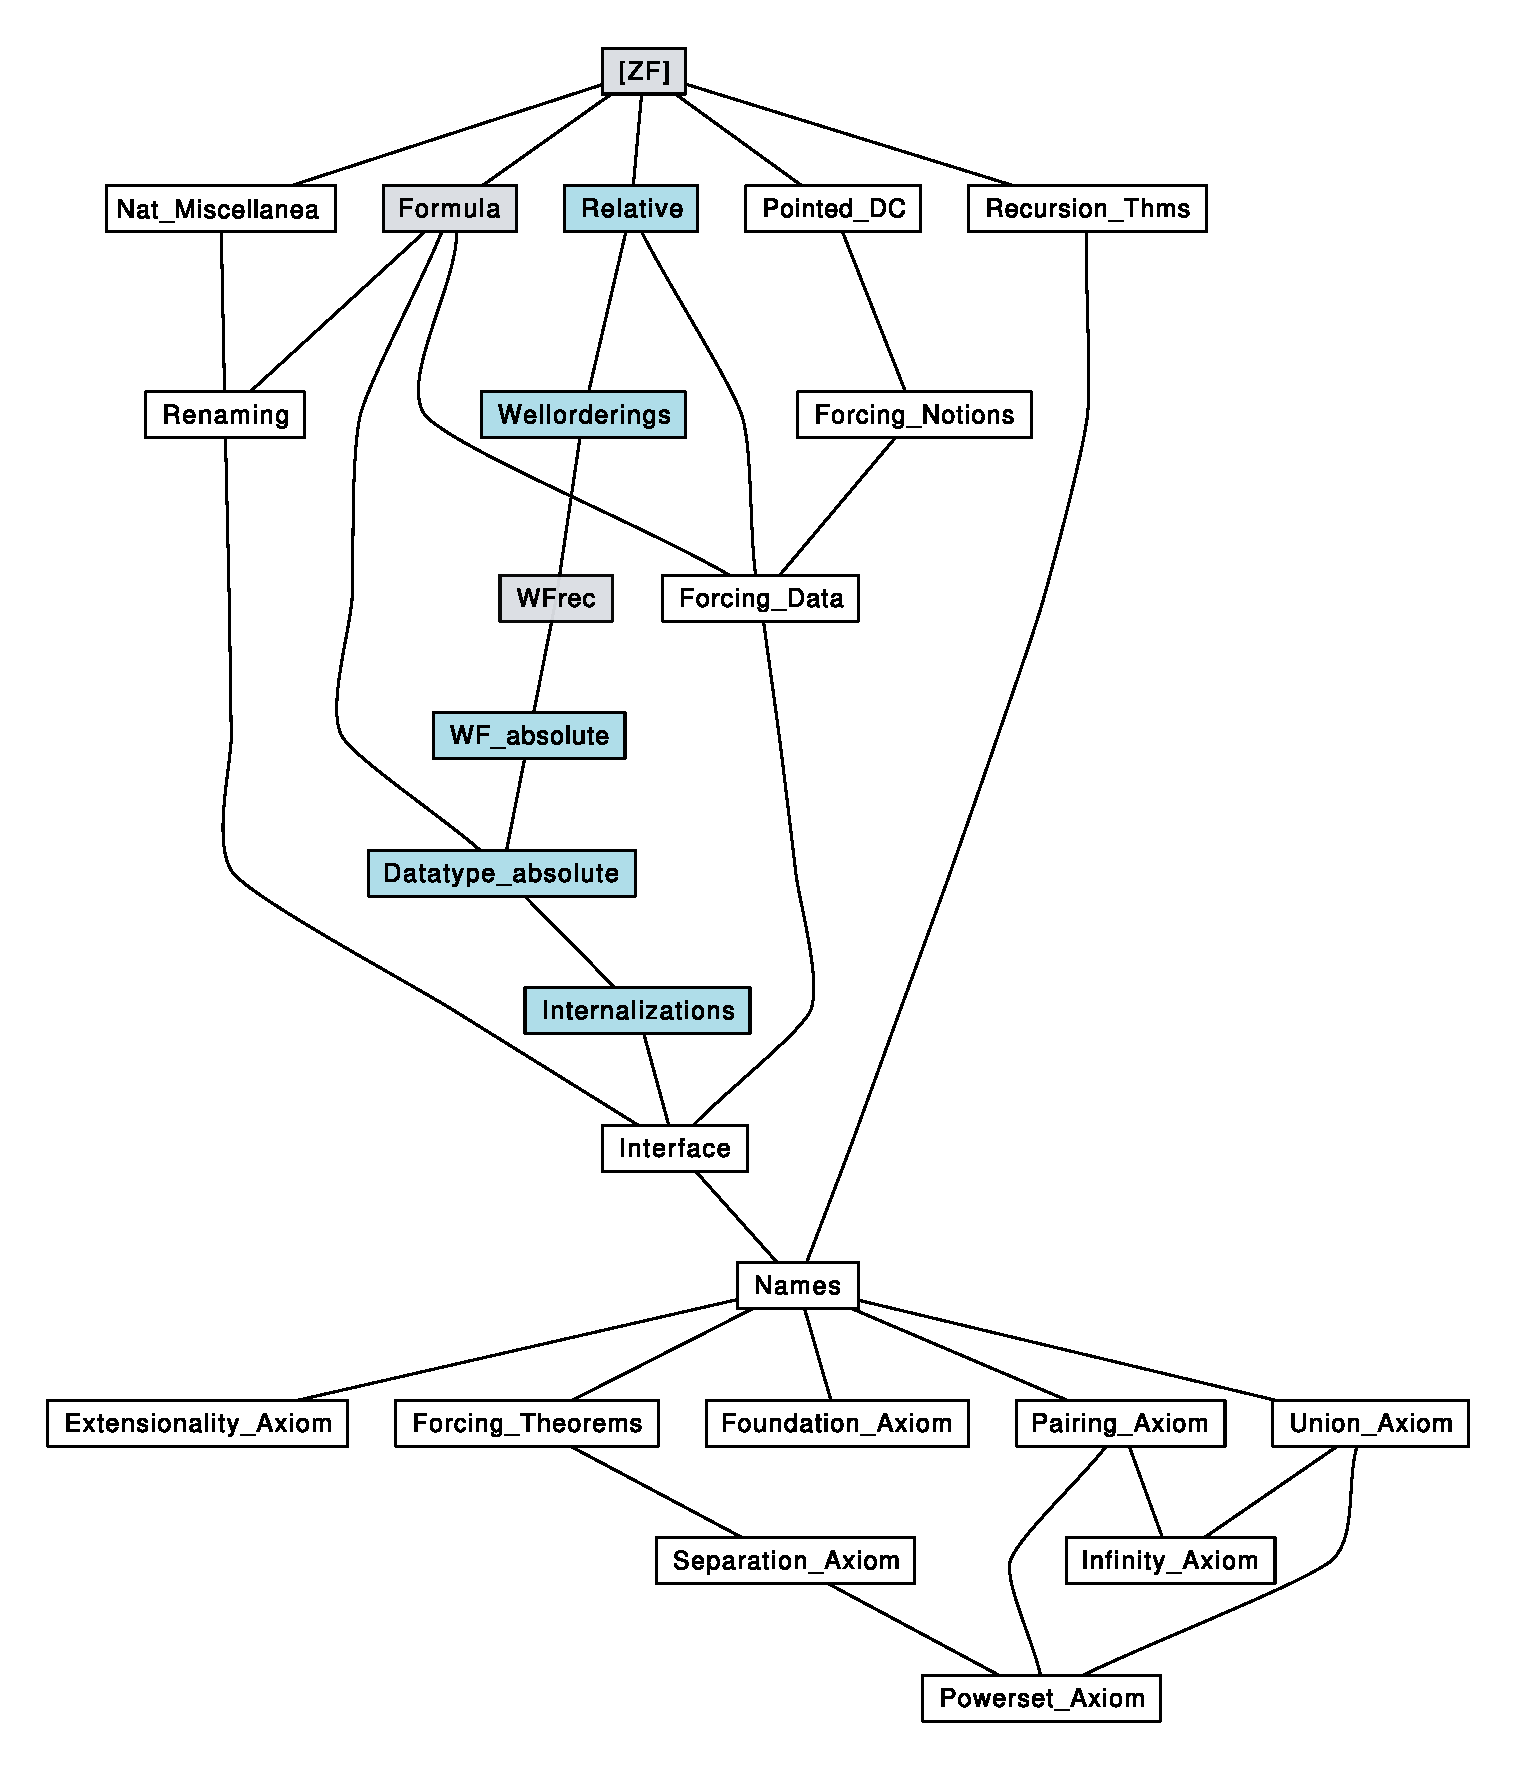
\includegraphics[height=14.8cm]{session_graph_colored.pdf}
  \end{center}
  \caption{Dependency graph of the \isatt{Separation} session.}
  \label{fig:deps}
\end{figure*}

%%% Local Variables: 
%%% mode: latex
%%% TeX-master: "Separation_In_MG"
%%% ispell-local-dictionary: "american"
%%% End: 

\end{document}

%%% Local Variables:
%%% mode: latex
%%% ispell-local-dictionary: "american"
%%% End:


\newpage
\appendix
\section*{A short overview of our development}
%%%%%%%%%%%%%%%%%%%%%%%%%%%%%%%%%%%
%% Appendix
%%%%%%%%%%%%%%%%%%%%%%%%%%%%%%%%%%%
In this appendix we succintly describe the contents of each file. We
include in 
Figure~\ref{fig:deps}  a dependency graph of our formalization. The
theories on a grayish background are directly from Paulson; we
highlight with blue/cyan those of Paulson that we modified. We
have developed from scratch the rest, in white.

\begin{description}
\item[\texttt{Nat\_Miscelanea}]Miscelaneous results for naturals, mostly
  needed for renamings.
\item[\texttt{Renaming}] Renaming of internalized formulas, see
  Section \ref{sec:renaming}.
\item[\texttt{Pointed\_DC}] A pointed version of the Principle of
  Dependent Choices.
\item[\texttt{Recursion\_Thms}] Enhancements about recursively defined
  functions.
\item[\texttt{Forcing\_Notions}] Definition of Posets with maximal
  element, filters, dense sets. Proof of Rasiowa-Sikorski.
\item[\texttt{Forcing\_Data}] Definition of the locales:
  \begin{inlinelist}
  \item \texttt{M\_ZF} satisfaction of axioms; and 
  \item \texttt{forcing\_data} extending the previous one with
    \texttt{forcing\_notion}, transitivity, and being countable.
  \end{inlinelist}
\item[\texttt{Interface}] Instantiation of locales \texttt{M\_trivial}
  and \texttt{M\_basic} for every instance of \texttt{Forcing\_Data}.
\item[\texttt{Names}] Definitions of $\chk$, $\val$, and the generic
  extension. Various results about them.
\item[\texttt{Forcing\_Theorems}] Specification of fundamental
  theorems of forcing, see Section~\ref{sec:forcing}.
\item[\texttt{*\_Axiom}] Proof of the satisfaction of the
  corresponding axiom in the generic extension.
\end{description}
%
\begin{figure*}[!b]
  \begin{center}
    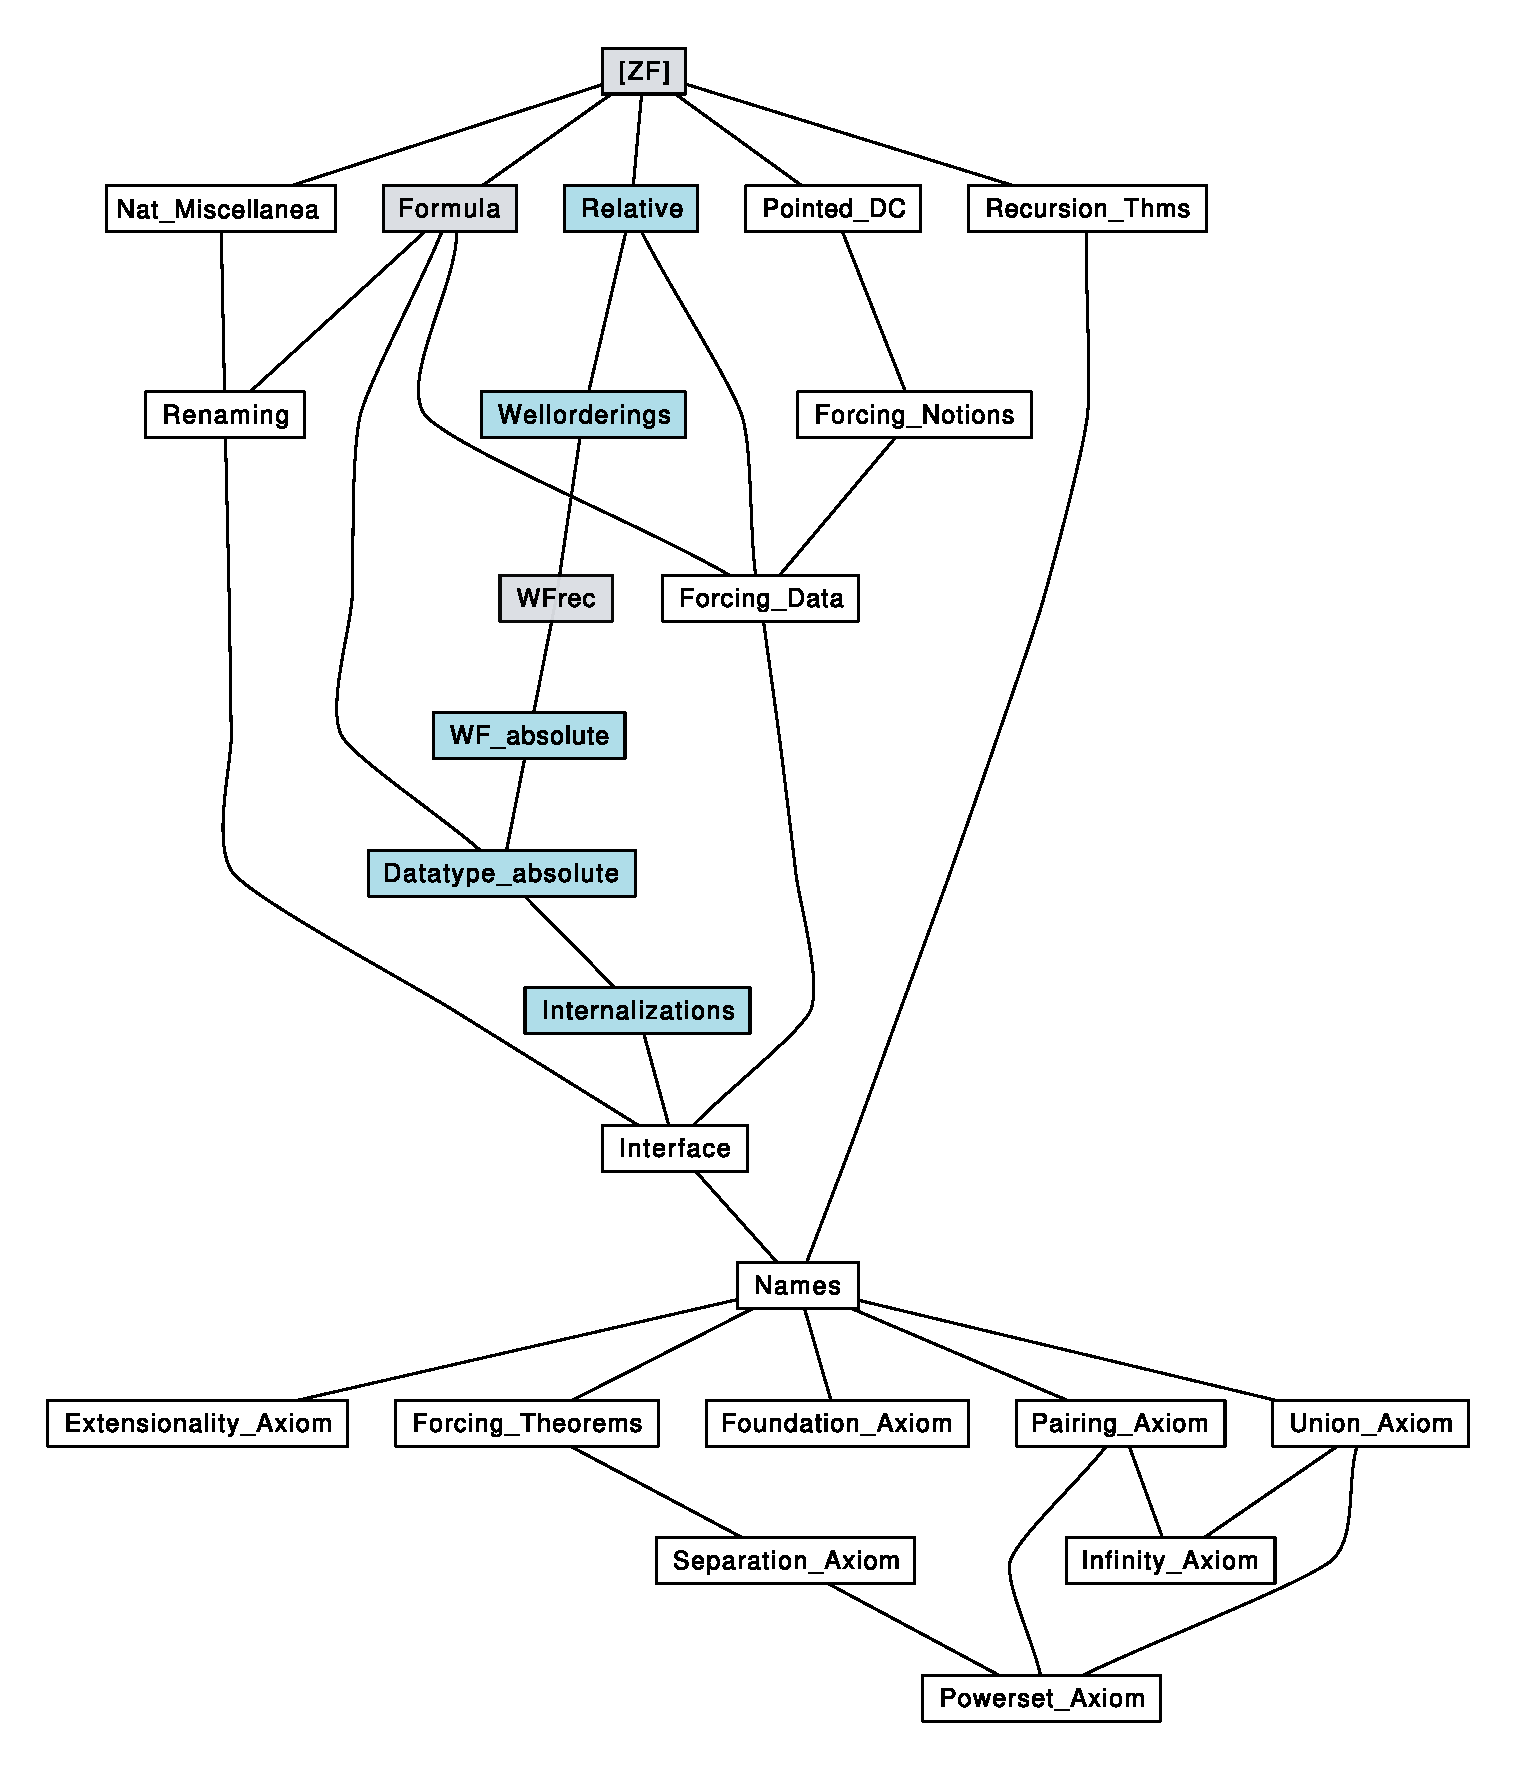
\includegraphics[height=14.8cm]{session_graph_colored.pdf}
  \end{center}
  \caption{Dependency graph of the \isatt{Separation} session.}
  \label{fig:deps}
\end{figure*}

%%% Local Variables: 
%%% mode: latex
%%% TeX-master: "Separation_In_MG"
%%% ispell-local-dictionary: "american"
%%% End: 

\end{document}

%%% Local Variables:
%%% mode: latex
%%% ispell-local-dictionary: "american"
%%% End:

\end{document}

%%% Local Variables:
%%% mode: latex
%%% ispell-local-dictionary: "american"
%%% End:
